% ============================================================
%  BÁO CÁO ĐỒ ÁN MÔN HỌC – AIRVNV
%  Engine: XeLaTeX (tốt nhất cho tiếng Việt + Unicode)
%  Compile: xelatex main.tex
% ============================================================
\documentclass[12pt, a4paper, oneside]{report}

% ── Font & Ngôn ngữ ─────────────────────────────────────────
\usepackage{fontspec}
\usepackage{polyglossia}
\setmainlanguage{vietnamese}
% TeX Gyre fonts — tương đương Times/Arial/Courier, có sẵn trong TeXLive
% Termes  ≈ Times New Roman  |  Heros ≈ Arial  |  Cursor ≈ Courier New
\setmainfont{TeX Gyre Termes}
\setsansfont{TeX Gyre Heros}
\setmonofont[Scale=0.9]{TeX Gyre Cursor}

% ── Căn lề chuẩn A4 học thuật ───────────────────────────────
\usepackage[
  a4paper,
  top=3cm, bottom=3cm,
  left=3.5cm, right=2cm,
  headheight=14.5pt
]{geometry}

% ── Dòng kẻ & Căn chỉnh ─────────────────────────────────────
\usepackage{setspace}
\onehalfspacing                   % Giãn dòng 1.5 chuẩn báo cáo

\usepackage{indentfirst}          % Thụt đầu dòng đoạn đầu chương
\setlength{\parindent}{1.27cm}
\setlength{\parskip}{6pt}

% ── Header / Footer ─────────────────────────────────────────
\usepackage{fancyhdr}
\pagestyle{fancy}
\fancyhf{}
\fancyhead[L]{\small\textit{Học viện Công nghệ Bưu chính Viễn thông}}
\fancyhead[R]{\small\textit{\leftmark}}
\fancyfoot[C]{\thepage}
\renewcommand{\headrulewidth}{0.4pt}

% ── Tiêu đề chương – viết hoa, căn giữa ────────────────────
\usepackage{titlesec}
\titleformat{\chapter}[display]
  {\normalfont\Large\bfseries\centering}
  {CHƯƠNG \thechapter}{0pt}{\Large\MakeUppercase}
\titlespacing*{\chapter}{0pt}{-20pt}{20pt}

\titleformat{\section}{\normalfont\large\bfseries}{\thesection}{1em}{}
\titleformat{\subsection}{\normalfont\normalsize\bfseries}{\thesubsection}{1em}{}

% ── Đánh số theo chương ─────────────────────────────────────
\usepackage{chngcntr}
\counterwithin{figure}{chapter}
\counterwithin{table}{chapter}
\counterwithin{equation}{chapter}

% ── Hình ảnh & Bảng ─────────────────────────────────────────
\usepackage{graphicx}
\usepackage{tabularx}
\graphicspath{{figures/}}
\usepackage{float}
\usepackage{caption}
\captionsetup{
  font=small,
  labelfont=bf,
  labelsep=period
}
\usepackage{subcaption}

\usepackage{booktabs}
\usepackage{tabularx}
\usepackage{longtable}
\usepackage{multirow}
\usepackage{array}

% ── Code listing ─────────────────────────────────────────────
\usepackage{listings}
\usepackage{xcolor}
\usepackage{colortbl}
\definecolor{codegray}{rgb}{0.95,0.95,0.95}
\definecolor{codeblue}{rgb}{0.0,0.3,0.6}
\lstset{
  backgroundcolor=\color{codegray},
  basicstyle=\ttfamily\footnotesize,
  breaklines=true,
  frame=single,
  keywordstyle=\color{codeblue}\bfseries,
  numbers=left,
  numberstyle=\tiny\color{gray},
  showstringspaces=false,
  captionpos=b
}

% ── Toán học ─────────────────────────────────────────────────
\usepackage{amsmath, amssymb}

% ── Hyperlink & PDF metadata ─────────────────────────────────
\usepackage[
  colorlinks=true,
  linkcolor=black,
  citecolor=black,
  urlcolor=blue,
  pdfencoding=auto,
  unicode=true
]{hyperref}
\usepackage{bookmark}

% ── Tài liệu tham khảo ──────────────────────────────────────
\usepackage[
  backend=biber,
  style=numeric,
  sorting=none
]{biblatex}
\addbibresource{appendix/tai_lieu_tham_khao.bib}

% ── Tiện ích khác ────────────────────────────────────────────
\usepackage{enumitem}
\usepackage{microtype}
\usepackage{tocbibind}            % Đưa tài liệu tham khảo vào mục lục
\usepackage{tocloft}              % Tùy chỉnh mục lục

% Mục lục dãn dòng chuẩn
\setlength{\cftbeforechapskip}{6pt}
\renewcommand{\cftchapfont}{\bfseries}
\renewcommand{\cftchappagefont}{\bfseries}

% ── Lệnh tiện ích nội bộ ─────────────────────────────────────
\newcommand{\todo}[1]{\textcolor{red}{\textbf{[TODO: #1]}}}
\newcommand{\placeholder}[1]{\textcolor{gray}{\textit{[#1]}}}

% ============================================================
\begin{document}

% ── Trang bìa (file riêng – bổ sung sau) ────────────────────
% \input{cover/00_bia}
% \cleardoublepage

% ── Lời cam đoan (nếu có) ───────────────────────────────────
% \input{cover/00_cam_doan}
% \cleardoublepage

% ── Mục lục ─────────────────────────────────────────────────
\tableofcontents
\cleardoublepage

% ── Danh mục hình vẽ ────────────────────────────────────────
\listoffigures
\cleardoublepage

% ── Danh mục bảng biểu ──────────────────────────────────────
\listoftables
\cleardoublepage

% ── Nội dung chính ──────────────────────────────────────────
% ============================================================
%  CHƯƠNG I: TỔNG QUAN
% ============================================================
\chapter{TỔNG QUAN}
\label{chap:tong_quan}

% ────────────────────────────────────────────────────────────
\section{Giới thiệu đề tài}
\label{sec:gioi_thieu}

\subsection{Bối cảnh}
\label{subsec:boi_canh}

Trong những năm gần đây, thị trường cho thuê nhà ngắn hạn tại Việt Nam và trên toàn cầu đã chứng kiến
sự tăng trưởng vượt bậc nhờ sự phổ biến của các nền tảng trực tuyến như Airbnb, Booking.com hay
Agoda. Mô hình này không chỉ tạo ra nguồn thu nhập thụ động cho chủ nhà mà còn cung cấp cho
khách du lịch những lựa chọn đa dạng, linh hoạt hơn so với khách sạn truyền thống.

Tuy nhiên, đằng sau giao diện người dùng đơn giản là những bài toán kỹ thuật phức tạp mà các
hệ thống này phải giải quyết:

\begin{itemize}
    \item \textbf{Tính toàn vẹn dữ liệu:} Một bất động sản không thể bị đặt trùng bởi hai khách
    hàng cùng lúc — đây là bài toán xử lý đồng thời (concurrency control) trong hệ thống phân tán.

    \item \textbf{Khả năng tìm kiếm theo địa lý:} Khách cần tìm phòng trong bán kính nhất định
    so với điểm du lịch — đòi hỏi hệ thống tìm kiếm địa không gian (geo-spatial search) hiệu năng cao.

    \item \textbf{Đồng bộ dữ liệu thời gian thực:} Khi chủ nhà cập nhật thông tin, kết quả tìm
    kiếm của khách phải phản ánh ngay lập tức mà không cần truy vấn trực tiếp vào cơ sở dữ liệu
    giao dịch.

    \item \textbf{Giao tiếp theo ngữ cảnh:} Hệ thống chat không đơn thuần là nhắn tin P2P mà phải
    được gắn chặt với ngữ cảnh nghiệp vụ (một bất động sản hoặc một đơn đặt phòng cụ thể).

    \item \textbf{Xử lý thanh toán an toàn:} Luồng thanh toán phải đảm bảo tính nguyên tử
    (atomicity) và không block hệ thống — kết quả thanh toán phải được xử lý bất đồng bộ.
\end{itemize}

Đề tài \textbf{AirVnV} ra đời từ nhu cầu nghiên cứu và xây dựng một nền tảng cho thuê nhà ngắn
hạn hiện đại, áp dụng kiến trúc phân tán để giải quyết các thách thức nêu trên trong điều kiện
thực tế. Đây không phải là bài toán học thuật đơn thuần mà là một bài toán kỹ thuật phần mềm
có tính ứng dụng cao.

\subsection{Mục tiêu}
\label{subsec:muc_tieu}

Mục tiêu của đồ án là xây dựng một nền tảng đặt phòng trực tuyến hoàn chỉnh — từ backend đến
frontend — với các chức năng cốt lõi gồm: quản lý bất động sản, tìm kiếm theo địa lý, đặt phòng,
thanh toán và chat theo ngữ cảnh.

Bên cạnh việc hoàn thiện sản phẩm về mặt chức năng, nhóm tập trung vào việc giải quyết
các bài toán kỹ thuật thực tế trong hệ thống phân tán:

\begin{itemize}
    \item Áp dụng kiến trúc Microservices — mỗi nghiệp vụ là một service độc lập, có thể
    phát triển và triển khai riêng lẻ.

    \item Đảm bảo tính nhất quán dữ liệu giữa các service mà không dùng distributed transaction,
    thông qua Transactional Outbox Pattern và Change Data Capture (CDC).

    \item Xây dựng hệ thống tìm kiếm địa lý hiệu năng cao bằng Elasticsearch — kết quả tìm kiếm
    không truy vấn trực tiếp vào database giao dịch.

    \item Xây dựng hệ thống chat real-time gắn với ngữ cảnh đặt phòng, tự động phát sinh
    thông báo hệ thống khi có sự kiện nghiệp vụ.

    \item Thiết kế luồng thanh toán bất đồng bộ — kết quả thanh toán không block luồng chính
    mà được xử lý qua message broker.
\end{itemize}

\subsubsection*{Phạm vi}

Đồ án bao gồm ba nhóm người dùng: Khách (Guest), Chủ nhà (Host) và Quản trị viên (Admin).
Ứng dụng mobile native nằm ngoài phạm vi của đồ án này.


% ────────────────────────────────────────────────────────────
\section{Cơ sở lý thuyết}
\label{sec:co_so_ly_thuyet}

Để giải quyết các bài toán đặt ra, đồ án áp dụng một tập hợp các công nghệ và kiến trúc hiện đại.
Phần này trình bày nền tảng lý thuyết của từng thành phần và lý do lựa chọn.

% ── 2.1 Microservices Architecture ──────────────────────────
\subsection{Kiến trúc Microservices}
\label{subsec:microservices}

Kiến trúc Microservices phân chia hệ thống thành các service nhỏ, độc lập, mỗi service chịu
trách nhiệm về một miền nghiệp vụ duy nhất và có cơ sở dữ liệu riêng (Database-per-Service).
Ngược lại với kiến trúc Monolith, Microservices cho phép:

\begin{itemize}
    \item Triển khai độc lập từng service mà không cần build lại toàn bộ hệ thống.
    \item Scale theo chiều ngang (horizontal scaling) có chọn lọc — chỉ scale service đang chịu tải cao.
    \item Cách ly lỗi (fault isolation): lỗi ở một service không làm sập toàn bộ hệ thống.
\end{itemize}

Trong AirVnV, hệ thống được phân rã thành 7 service: \textit{UserService, PropertyService,
SearchService, BookingService, PaymentService, ChatService} và \textit{Gateway}.

% ── 2.2 API Gateway Pattern ─────────────────────────────────
\subsection{API Gateway Pattern}
\label{subsec:api_gateway}

API Gateway là một điểm vào duy nhất (single entry point) cho tất cả các yêu cầu từ client.
Gateway đảm nhận các trách nhiệm:

\begin{itemize}
    \item \textbf{Routing:} Định tuyến request đến đúng service.
    \item \textbf{Authentication:} Xác thực JWT token trước khi forward request.
    \item \textbf{Load Balancing:} Phân phối tải đến các instance của cùng một service.
\end{itemize}

Đồ án sử dụng \textbf{YARP} (Yet Another Reverse Proxy) — một thư viện reverse proxy hiệu năng cao
được phát triển bởi Microsoft, tích hợp tốt với .NET ecosystem và .NET Aspire.

% ── 2.3 CQRS và Mediator Pattern ────────────────────────────
\subsection{CQRS và Mediator Pattern}
\label{subsec:cqrs_mediator}

\textbf{CQRS (Command Query Responsibility Segregation)} là pattern tách biệt hoàn toàn luồng ghi dữ liệu (Command) và luồng đọc dữ liệu (Query).
Mỗi thao tác nghiệp vụ được biểu diễn bằng một object (Command hoặc Query) và xử lý bởi một Handler tương ứng.

\begin{itemize}
    \item \textbf{Command:} Thay đổi trạng thái hệ thống. Ví dụ: \texttt{CreateBookingCommand},
    \texttt{PublishPropertyCommand}.
    \item \textbf{Query:} Chỉ đọc dữ liệu, không có side-effect. Ví dụ: \texttt{GetPropertyQuery},
    \texttt{SearchPropertiesQuery}.
\end{itemize}

Để triển khai CQRS một cách hiệu quả và giảm thiểu sự phụ thuộc chéo (coupling) giữa các class, đồ án áp dụng \textbf{Mediator Pattern} (thông qua thư viện \texttt{Mediator.SourceGenerator}).
Mediator Pattern đóng vai trò là một "người điều phối" trung tâm. Thay vì các Endpoint/Controller phải tiêm (inject) hàng loạt các Service/Repository gây ra tình trạng "God object",
chúng chỉ cần gửi (Send) một \texttt{Request} tới Mediator. Mediator sẽ dựa vào kiểu dữ liệu của Request để tự động định tuyến tới đúng \texttt{Handler} duy nhất chịu trách nhiệm xử lý.

Sự kết hợp giữa CQRS, Mediator Pattern và \textbf{FastEndpoints} giúp hệ thống hiện thực hóa mô hình kiến trúc cắt dọc (\textbf{Vertical Slice Architecture}).
Theo đó, mỗi Use Case nghiệp vụ được gom cụm độc lập trong một thư mục duy nhất (gồm \texttt{Endpoint.cs, Request.cs, Response.cs, Handler.cs}),
tối đa hóa tính gắn kết nội bộ (high cohesion) và hạn chế tối đa rủi ro khi thay đổi mã nguồn.

% ── 2.4 Event-Driven Architecture ───────────────────────────
\subsection{Kiến trúc Hướng sự kiện (Event-Driven Architecture)}
\label{subsec:eda}

Event-Driven Architecture (EDA) là mô hình các service giao tiếp với nhau thông qua việc
phát và tiêu thụ sự kiện (events) bất đồng bộ thay vì gọi trực tiếp (synchronous HTTP).

Trong AirVnV, hai message broker được sử dụng với vai trò khác nhau:

\begin{itemize}
    \item \textbf{RabbitMQ:} Dùng cho Domain Events nội bộ — các sự kiện nghiệp vụ ngắn hạn
    giữa các service (ví dụ: \texttt{BookingConfirmedEvent} kích hoạt ChatService inject
    system message).

    \item \textbf{Apache Kafka:} Dùng cho Data Streaming — luồng dữ liệu lớn, bền vững, hỗ
    trợ replay. Cụ thể là luồng CDC từ PostgreSQL đến Elasticsearch.
\end{itemize}

% ── 2.5 Transactional Outbox Pattern ────────────────────────
\subsection{Transactional Outbox Pattern}
\label{subsec:outbox}

Một thách thức cốt lõi của Microservices là: làm sao đảm bảo rằng khi một nghiệp vụ thành công
(ví dụ: lưu Booking vào DB), sự kiện tương ứng (ví dụ: \texttt{BookingCreatedEvent}) luôn
được publish đến message broker — kể cả khi ứng dụng crash ngay sau khi lưu DB?

Outbox Pattern giải quyết vấn đề này bằng cách lưu event vào một bảng \texttt{OutboxMessage}
trong \textit{cùng một transaction} với nghiệp vụ chính. Một background worker riêng biệt
sẽ đọc bảng Outbox và publish event đến broker, đảm bảo tính nguyên tử (atomicity) mà không
cần distributed transaction.

% ── 2.6 Change Data Capture ─────────────────────────────────
\subsection{Change Data Capture (CDC) với Debezium}
\label{subsec:cdc}

CDC là kỹ thuật theo dõi các thay đổi trong cơ sở dữ liệu (INSERT, UPDATE, DELETE) ở
mức transaction log và phát chúng ra ngoài như các sự kiện.

Đồ án sử dụng \textbf{Debezium} — một nền tảng CDC mã nguồn mở — để đọc Write-Ahead Log (WAL)
của PostgreSQL và publish các thay đổi vào Kafka. SearchService tiêu thụ luồng Kafka này để
cập nhật Elasticsearch, đảm bảo read-model luôn đồng bộ gần thời gian thực với dữ liệu giao dịch.

% ── 2.7 Geo-Spatial Search ──────────────────────────────────
\subsection{Tìm kiếm và Chỉ mục với Elasticsearch}
\label{subsec:geo_search}

Elasticsearch là một công cụ tìm kiếm và phân tích phân tán (Distributed Search Engine) dựa trên Apache Lucene.
Thay vì lưu dữ liệu dạng bảng như RDBMS và sử dụng phép toán \texttt{LIKE} vốn cực kỳ chậm chạp trên tập dữ liệu lớn,
Elasticsearch sử dụng cấu trúc \textbf{Inverted Index} (Chỉ mục ngược). Cấu trúc này ánh xạ từng từ khóa (token)
ngược lại với các tài liệu (documents) chứa từ khóa đó, giúp tốc độ tìm kiếm văn bản toàn văn (Full-text Search)
nhanh gấp hàng trăm lần SQL.

Bên cạnh đó, Elasticsearch hỗ trợ mạnh mẽ kiểu dữ liệu \texttt{geo\_point}, cho phép thực hiện các truy vấn
không gian (Geo-Spatial) phức tạp như:
\begin{itemize}
    \item \textbf{Geo Distance Query:} Tìm tất cả bất động sản trong bán kính $r$ km từ một tọa độ GPS $(lat, lon)$.
    \item \textbf{Geo Bounding Box:} Lọc các bất động sản nằm lọt thỏm trong một vùng khung chữ nhật trên bản đồ.
\end{itemize}
Thông qua thư viện client \texttt{Aspire.Elastic.Clients.Elasticsearch}, \texttt{SearchService} thao tác trực tiếp với
Elasticsearch dưới dạng Read-Model. Việc tách biệt hoàn toàn cơ sở dữ liệu đọc (Elasticsearch) và ghi (PostgreSQL)
giúp hiệu năng tìm kiếm đạt được tốc độ cực cao, $O(1)$, bất chấp sự gia tăng của lượng dữ liệu.

% ── 2.8 .NET Aspire ─────────────────────────────────────────
\subsection{.NET Aspire — Service Discovery và Orchestration}
\label{subsec:aspire}

.NET Aspire là nền tảng orchestration của Microsoft dành cho ứng dụng phân tán. Thay vì
hardcode connection string và URL giữa các service, Aspire cung cấp:

\begin{itemize}
    \item \textbf{Service Discovery:} Các service tìm thấy nhau bằng tên logic
    (ví dụ: \texttt{http://property-service/...}) thay vì IP/port cứng.
    \item \textbf{Infrastructure Provisioning:} Aspire tự động khởi động các container
    (PostgreSQL, Redis, Kafka, RabbitMQ, Elasticsearch) khi chạy môi trường phát triển.
    \item \textbf{Observability Dashboard:} Giao diện theo dõi logs, metrics và traces
    tập trung cho toàn bộ hệ thống.
\end{itemize}

% ── 2.9 Hệ quản trị CSDL PostgreSQL & ORM ───────────────────
\subsection{Hệ quản trị Cơ sở dữ liệu PostgreSQL và ORM}
\label{subsec:db_orm}

\textbf{PostgreSQL} được lựa chọn làm hệ quản trị cơ sở dữ liệu quan hệ (RDBMS) chính cho các Microservices.
Lý do chính bao gồm: tính tuân thủ ACID nghiêm ngặt giúp đảm bảo toàn vẹn dữ liệu tài chính (Booking, Payment),
và khả năng hỗ trợ kiểu dữ liệu \texttt{JSONB} mạnh mẽ. \texttt{JSONB} cho phép lưu trữ các trường dữ liệu bán cấu trúc
(semi-structured data) như danh sách tiện ích (amenities) hoặc bộ lọc tìm kiếm một cách linh hoạt mà không cần
chuẩn hóa quá mức (over-normalization).

Để giao tiếp với PostgreSQL, đồ án sử dụng \textbf{Entity Framework Core} (EF Core) thông qua thư viện \texttt{Npgsql.EntityFrameworkCore.PostgreSQL}.
EF Core là một Object-Relational Mapper (ORM) mạnh mẽ, cung cấp cơ chế Code-First Migrations, giúp
tự động hóa việc tạo và cập nhật schema cơ sở dữ liệu. Để đảm bảo nguyên tắc \textit{Database-per-service},
mỗi Microservice duy trì một lịch sử Migration độc lập và tự động apply vào Logical Database của riêng nó
ngay khi khởi động.

% ── 2.10 Hệ thống Real-time với SignalR & Redis Backplane ───
\subsection{Hệ thống Thời gian thực với SignalR và Redis Backplane}
\label{subsec:signalr_redis}

Chức năng nhắn tin (Chat) và thông báo (Notification) đòi hỏi kết nối hai chiều liên tục giữa Server và Client
với độ trễ cực thấp. Để đáp ứng nhu cầu này, đồ án sử dụng \textbf{SignalR} (\texttt{Microsoft.AspNetCore.SignalR}).
SignalR tự động quản lý các kết nối WebSocket (và fallback xuống Server-Sent Events hoặc Long Polling nếu cần),
cho phép máy chủ đẩy dữ liệu (push) trực tiếp đến các client đang kết nối.

Tuy nhiên, trong môi trường phân tán (Docker/Kubernetes), \texttt{ChatService} có thể được nhân bản (scale-out) thành nhiều node.
Nếu User A kết nối tới Node 1 và User B kết nối tới Node 2, Node 1 sẽ không biết cách gửi tin nhắn trực tiếp cho User B.
Để giải quyết rào cản này, \textbf{Redis Backplane} (\texttt{StackExchange.Redis}) được tích hợp.
Mọi tin nhắn SignalR gửi ra sẽ được đẩy vào kênh Redis Pub/Sub; sau đó Redis sẽ broadcast tin nhắn này tới tất cả
các node của \texttt{ChatService}, đảm bảo tin nhắn luôn đến đúng người nhận bất kể họ đang duy trì socket với node nào.

% ── 2.11 Bảo mật, Định tuyến và Ánh xạ Dữ liệu ──────────────
\subsection{Bảo mật, Thiết kế API và Ánh xạ dữ liệu}
\label{subsec:security_mapping}

\begin{itemize}
    \item \textbf{Thiết kế API siêu tốc (FastEndpoints):} Thay vì sử dụng mô hình MVC/Controllers truyền thống vốn
    cồng kềnh, hệ thống sử dụng thư viện \texttt{FastEndpoints}. Thư viện này triển khai kiến trúc REPR
    (Request-Endpoint-Response), giúp nhóm (group) tất cả logic nghiệp vụ, validation và routing của một API vào một file duy nhất,
    tối ưu tốc độ thực thi và cực kỳ dễ dàng bảo trì.
    
    \item \textbf{Bảo mật \& Xác thực (Security):} Hệ thống kết hợp \textbf{JSON Web Token (JWT)} để xác thực không
    trạng thái (stateless authentication) qua YARP Gateway. Mật khẩu người dùng được băm (hash) an toàn bằng thuật toán bcrypt qua thư viện
    \texttt{BCrypt.Net-Next}. Đồng thời, đồ án tích hợp hệ thống đăng nhập một chạm (SSO) qua Google nhờ các thư viện
    \texttt{FirebaseAdmin} và \texttt{Google.Apis.Auth}.
    
    \item \textbf{Ánh xạ dữ liệu (Mapster):} Trong kiến trúc sạch, dữ liệu phải được ánh xạ liên tục giữa Entity và DTO. 
    Thay vì dùng AutoMapper (dựa trên Reflection làm suy giảm hiệu năng), hệ thống sử dụng \texttt{Mapster}.
    Mapster sinh mã trực tiếp lúc biên dịch (code generation), giúp tốc độ chuyển đổi dữ liệu đạt mức tối đa.
\end{itemize}

% ── 2.12 Tích hợp Thanh toán Ngoại vi ───────────────────────
\subsection{Tích hợp Cổng thanh toán Ngoại vi (Payment Gateway)}
\label{subsec:payment_gateway}

Luồng thanh toán trong AirVnV không lưu trữ trực tiếp thông tin thẻ tín dụng nhằm giảm tải rủi ro pháp lý và
đảm bảo tuân thủ tiêu chuẩn PCI-DSS. Thay vào đó, \texttt{PaymentService} tích hợp với nền tảng \textbf{Stripe} thông qua thư viện \texttt{Stripe.net} (hoặc VNPay).

Khi khách hàng khởi tạo thanh toán, hệ thống sẽ sinh ra một Payment Session và điều hướng người dùng sang giao diện an toàn của đối tác.
Mấu chốt của kiến trúc thanh toán phân tán là cơ chế \textbf{Webhook}: Hệ thống thanh toán sẽ gọi ngược (callback)
về hệ thống AirVnV thông qua một API đặc biệt được bảo mật bằng chữ ký số (Webhook Signature) để báo cáo kết quả giao dịch.
Nhờ luồng xử lý này, hệ thống backend không bao giờ bị "treo" (block) để chờ kết quả giao dịch, đảm bảo tính bất đồng bộ 
và chống rớt đơn hàng hiệu quả kể cả khi kết nối mạng từ client bị ngắt ngang.

% ============================================================
%  CHƯƠNG II: THIẾT KẾ HỆ THỐNG
% ============================================================
\chapter{THIẾT KẾ HỆ THỐNG}
\label{chap:thiet_ke}

% ────────────────────────────────────────────────────────────
\section{Phân tích yêu cầu hệ thống}
\label{sec:phan_tich_yeu_cau}

% ── 1.1 Yêu cầu chức năng ───────────────────────────────────
\subsection{Yêu cầu chức năng (Functional Requirements)}
\label{subsec:yeu_cau_chuc_nang}

%
% REQUIREMENT (từ main.md – Chương II, mục 1.1):
%   - Vẽ Use Case Diagram tổng thể cho toàn hệ thống.
%     Actors: Khách (Guest), Chủ nhà (Host), Admin, Hệ thống (System).
%   - Đặc tả chi tiết các luồng nghiệp vụ chính bằng bảng Use Case:
%       + UC-01..05: Xác thực & Tài khoản
%       + UC-06..10: Quản lý bất động sản (Host đăng tin, sửa tin...)
%       + UC-11..15: Tìm kiếm & Đặt phòng (Guest)
%       + UC-16..20: Thanh toán & Hoàn tiền
%       + UC-21..25: Đánh giá & Tin nhắn
%       + UC-26..30: Quản trị hệ thống (Admin)
%   - Mỗi Use Case đặc tả đầy đủ: Actors, Pre/Post conditions,
%     Basic Flow, Alternative Flow, FR để dò vết.
%   - Tham chiếu chuẩn: file .agents/rules/reports/1. Cách viết Usecase.md
%

\subsubsection{Sơ đồ Use Case Tổng thể (Overview Use Case Diagram)}
Sơ đồ dưới đây minh họa các nhóm nghiệp vụ chính của hệ thống AirVnV, được phân bổ cho 4 nhóm Tác nhân (Actors) cốt lõi: Khách (Guest), Chủ nhà (Host), Quản trị viên (Admin), và Hệ thống (System).

\begin{figure}[H]
  \centering
  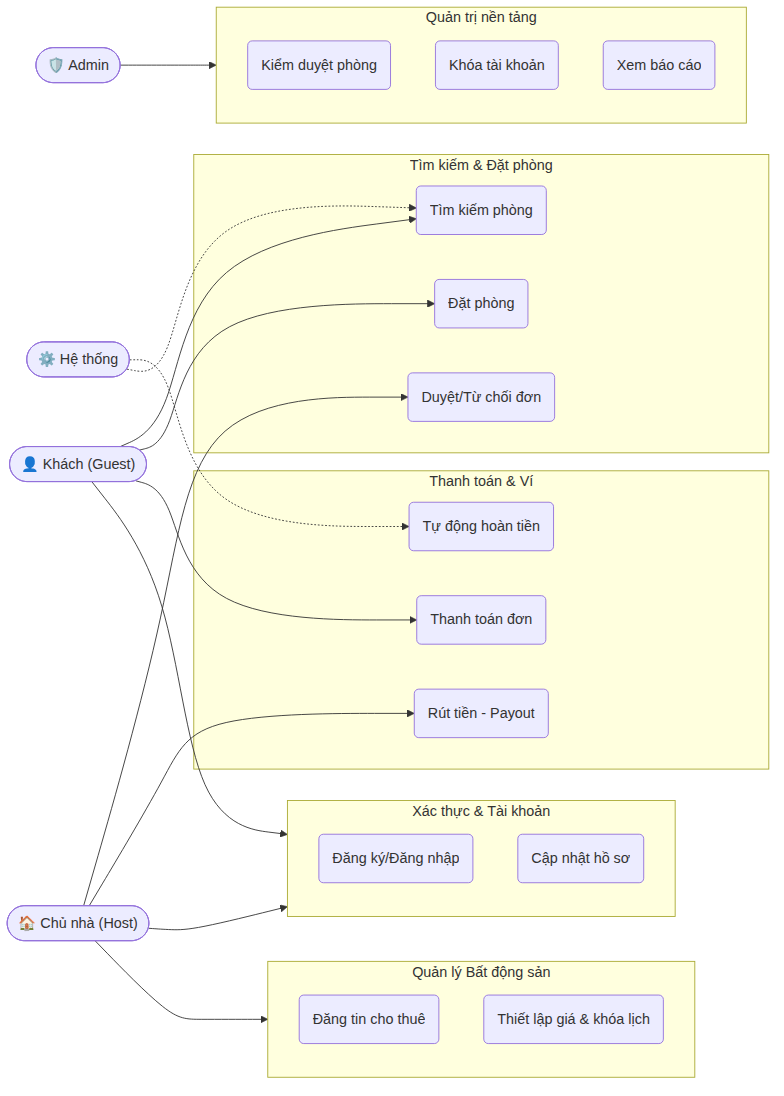
\includegraphics[width=\textwidth, height=10cm, keepaspectratio]{outputs/usecase_diagram.png}
  \caption{Sơ đồ Use Case Tổng quát của hệ thống AirVnV}
  \label{fig:usecase_diagram}
\end{figure}

\subsubsection{Đặc tả Use Case Chi tiết}
Dưới đây là đặc tả chi tiết 45 luồng nghiệp vụ cốt lõi (Use Cases) của hệ thống AirVnV, được ánh xạ trực tiếp từ các tài nguyên API (Endpoints) và được chia thành 7 nhóm chức năng (Features) độc lập nhằm đáp ứng yêu cầu của nền tảng phân tán.


\begin{table}[H]
\renewcommand{\arraystretch}{1.3}
\centering
\begin{tabularx}{\textwidth}{|p{4.5cm}|X|}
\hline
\cellcolor{gray!15}\bfseries Mã Usecase & \textbf{UC-01} \\ \hline
\cellcolor{gray!15}\bfseries Tên Usecase & \textbf{Đăng ký tài khoản} \\ \hline
\cellcolor{gray!15}\bfseries Tác nhân (Actors) & Khách (Guest), Chủ nhà (Host) \\ \hline
\cellcolor{gray!15}\bfseries Mô tả ngắn & Người dùng đăng ký tài khoản mới trên hệ thống AirVnV. \\ \hline
\cellcolor{gray!15}\bfseries Điều kiện tiên quyết & Người dùng chưa đăng nhập. \\ \hline
\cellcolor{gray!15}\bfseries Điều kiện đảm bảo & Tài khoản được tạo ở trạng thái Inactive, OTP được gửi qua email. \\ \hline
\cellcolor{gray!15}\bfseries Luồng sự kiện chính & 1. Người dùng nhập thông định cơ bản.\newline 2. Hệ thống kiểm tra email.\newline 3. Hệ thống tạo user và gửi OTP. \\ \hline
\cellcolor{gray!15}\bfseries Luồng rẽ nhánh & \textbf{Email đã tồn tại}: Hệ thống báo lỗi Email already exists. \\ \hline
\cellcolor{gray!15}\bfseries Yêu cầu chức năng (FR) & $\diamond$ \textbf{FR\_01.1}: Hệ thống từ chối nếu email trùng lặp. \\ \hline
\end{tabularx}
\end{table}

\begin{table}[H]
\renewcommand{\arraystretch}{1.3}
\centering
\begin{tabularx}{\textwidth}{|p{4.5cm}|X|}
\hline
\cellcolor{gray!15}\bfseries Mã Usecase & \textbf{UC-02} \\ \hline
\cellcolor{gray!15}\bfseries Tên Usecase & \textbf{Xác thực Email (Verify)} \\ \hline
\cellcolor{gray!15}\bfseries Tác nhân (Actors) & Người dùng \\ \hline
\cellcolor{gray!15}\bfseries Mô tả ngắn & Người dùng nhập mã OTP để kích hoạt tài khoản. \\ \hline
\cellcolor{gray!15}\bfseries Điều kiện tiên quyết & Tài khoản ở trạng thái Inactive, có mã OTP hợp lệ. \\ \hline
\cellcolor{gray!15}\bfseries Điều kiện đảm bảo & Tài khoản chuyển sang trạng thái Active. \\ \hline
\cellcolor{gray!15}\bfseries Luồng sự kiện chính & 1. Người dùng nhập OTP.\newline 2. Hệ thống kiểm tra tính hợp lệ.\newline 3. Cập nhật trạng thái Active. \\ \hline
\cellcolor{gray!15}\bfseries Luồng rẽ nhánh & \textbf{Mã hết hạn}: Hệ thống báo lỗi Verification code expired. \\ \hline
\cellcolor{gray!15}\bfseries Yêu cầu chức năng (FR) & $\diamond$ \textbf{FR\_02.1}: Mã OTP chỉ có hiệu lực trong 15 phút. \\ \hline
\end{tabularx}
\end{table}

\begin{table}[H]
\renewcommand{\arraystretch}{1.3}
\centering
\begin{tabularx}{\textwidth}{|p{4.5cm}|X|}
\hline
\cellcolor{gray!15}\bfseries Mã Usecase & \textbf{UC-03} \\ \hline
\cellcolor{gray!15}\bfseries Tên Usecase & \textbf{Đăng nhập hệ thống} \\ \hline
\cellcolor{gray!15}\bfseries Tác nhân (Actors) & Người dùng \\ \hline
\cellcolor{gray!15}\bfseries Mô tả ngắn & Người dùng đăng nhập bằng mật khẩu hoặc Google SSO. \\ \hline
\cellcolor{gray!15}\bfseries Điều kiện tiên quyết & Tài khoản đã kích hoạt. \\ \hline
\cellcolor{gray!15}\bfseries Điều kiện đảm bảo & Nhận được JWT Token để truy cập hệ thống. \\ \hline
\cellcolor{gray!15}\bfseries Luồng sự kiện chính & 1. Người dùng nhập email/mật khẩu.\newline 2. Hệ thống kiểm tra hash.\newline 3. Hệ thống cấp phát JWT Token. \\ \hline
\cellcolor{gray!15}\bfseries Luồng rẽ nhánh & \textbf{Sai mật khẩu}: Báo lỗi Invalid email or password. \\ \hline
\cellcolor{gray!15}\bfseries Yêu cầu chức năng (FR) & $\diamond$ \textbf{FR\_03.1}: Mật khẩu phải được mã hóa trước khi so sánh. \\ \hline
\end{tabularx}
\end{table}

\begin{table}[H]
\renewcommand{\arraystretch}{1.3}
\centering
\begin{tabularx}{\textwidth}{|p{4.5cm}|X|}
\hline
\cellcolor{gray!15}\bfseries Mã Usecase & \textbf{UC-04} \\ \hline
\cellcolor{gray!15}\bfseries Tên Usecase & \textbf{Cập nhật hồ sơ cá nhân} \\ \hline
\cellcolor{gray!15}\bfseries Tác nhân (Actors) & Người dùng \\ \hline
\cellcolor{gray!15}\bfseries Mô tả ngắn & Thay đổi thông tin như tên, ảnh đại diện, số điện thoại. \\ \hline
\cellcolor{gray!15}\bfseries Điều kiện tiên quyết & Người dùng đã đăng nhập. \\ \hline
\cellcolor{gray!15}\bfseries Điều kiện đảm bảo & Thông tin mới được lưu trữ trong CSDL. \\ \hline
\cellcolor{gray!15}\bfseries Luồng sự kiện chính & 1. Người dùng sửa thông tin.\newline 2. Hệ thống validate.\newline 3. Cập nhật CSDL. \\ \hline
\cellcolor{gray!15}\bfseries Luồng rẽ nhánh & \textbf{Lỗi định dạng}: Báo lỗi Validation Failed (400). \\ \hline
\cellcolor{gray!15}\bfseries Yêu cầu chức năng (FR) & $\diamond$ \textbf{FR\_04.1}: Số điện thoại phải đúng định dạng quốc gia. \\ \hline
\end{tabularx}
\end{table}

\begin{table}[H]
\renewcommand{\arraystretch}{1.3}
\centering
\begin{tabularx}{\textwidth}{|p{4.5cm}|X|}
\hline
\cellcolor{gray!15}\bfseries Mã Usecase & \textbf{UC-05} \\ \hline
\cellcolor{gray!15}\bfseries Tên Usecase & \textbf{Đổi mật khẩu} \\ \hline
\cellcolor{gray!15}\bfseries Tác nhân (Actors) & Người dùng \\ \hline
\cellcolor{gray!15}\bfseries Mô tả ngắn & Người dùng đang đăng nhập muốn đổi mật khẩu mới. \\ \hline
\cellcolor{gray!15}\bfseries Điều kiện tiên quyết & Đã đăng nhập. \\ \hline
\cellcolor{gray!15}\bfseries Điều kiện đảm bảo & Mật khẩu được cập nhật, các phiên đăng nhập khác bị đăng xuất. \\ \hline
\cellcolor{gray!15}\bfseries Luồng sự kiện chính & 1. Nhập mật khẩu cũ và mới.\newline 2. Hệ thống kiểm tra.\newline 3. Cập nhật mật khẩu. \\ \hline
\cellcolor{gray!15}\bfseries Luồng rẽ nhánh & \textbf{Sai mật khẩu cũ}: Báo lỗi và từ chối cập nhật. \\ \hline
\cellcolor{gray!15}\bfseries Yêu cầu chức năng (FR) & $\diamond$ \textbf{FR\_05.1}: Mật khẩu mới phải mạnh (có ký tự đặc biệt, hoa, thường). \\ \hline
\end{tabularx}
\end{table}

\begin{table}[H]
\renewcommand{\arraystretch}{1.3}
\centering
\begin{tabularx}{\textwidth}{|p{4.5cm}|X|}
\hline
\cellcolor{gray!15}\bfseries Mã Usecase & \textbf{UC-06} \\ \hline
\cellcolor{gray!15}\bfseries Tên Usecase & \textbf{Quên mật khẩu} \\ \hline
\cellcolor{gray!15}\bfseries Tác nhân (Actors) & Người dùng \\ \hline
\cellcolor{gray!15}\bfseries Mô tả ngắn & Yêu cầu khôi phục mật khẩu qua email. \\ \hline
\cellcolor{gray!15}\bfseries Điều kiện tiên quyết & Không yêu cầu đăng nhập. \\ \hline
\cellcolor{gray!15}\bfseries Điều kiện đảm bảo & Gửi link reset kèm token vào email. \\ \hline
\cellcolor{gray!15}\bfseries Luồng sự kiện chính & 1. Người dùng nhập email.\newline 2. Hệ thống tạo Reset Token.\newline 3. Gửi email chứa link khôi phục. \\ \hline
\cellcolor{gray!15}\bfseries Luồng rẽ nhánh & \textbf{Email không tồn tại}: Trả về 200 OK nhưng không gửi mail để tránh lộ thông tin. \\ \hline
\cellcolor{gray!15}\bfseries Yêu cầu chức năng (FR) & $\diamond$ \textbf{FR\_06.1}: Token reset chỉ có hiệu lực 1 lần duy nhất trong 30 phút. \\ \hline
\end{tabularx}
\end{table}

\begin{table}[H]
\renewcommand{\arraystretch}{1.3}
\centering
\begin{tabularx}{\textwidth}{|p{4.5cm}|X|}
\hline
\cellcolor{gray!15}\bfseries Mã Usecase & \textbf{UC-07} \\ \hline
\cellcolor{gray!15}\bfseries Tên Usecase & \textbf{Làm mới Token (Refresh Token)} \\ \hline
\cellcolor{gray!15}\bfseries Tác nhân (Actors) & Người dùng \\ \hline
\cellcolor{gray!15}\bfseries Mô tả ngắn & Lấy JWT mới khi token cũ hết hạn. \\ \hline
\cellcolor{gray!15}\bfseries Điều kiện tiên quyết & Sở hữu Refresh Token hợp lệ. \\ \hline
\cellcolor{gray!15}\bfseries Điều kiện đảm bảo & Cấp JWT mới và Refresh Token mới. \\ \hline
\cellcolor{gray!15}\bfseries Luồng sự kiện chính & 1. Client gửi Refresh Token.\newline 2. Hệ thống kiểm tra.\newline 3. Trả về bộ token mới. \\ \hline
\cellcolor{gray!15}\bfseries Luồng rẽ nhánh & \textbf{Token bị thu hồi}: Báo lỗi Token is revoked và yêu cầu đăng nhập lại. \\ \hline
\cellcolor{gray!15}\bfseries Yêu cầu chức năng (FR) & $\diamond$ \textbf{FR\_07.1}: Cơ chế xoay vòng (Rotation) Refresh Token để chống đánh cắp. \\ \hline
\end{tabularx}
\end{table}

\begin{table}[H]
\renewcommand{\arraystretch}{1.3}
\centering
\begin{tabularx}{\textwidth}{|p{4.5cm}|X|}
\hline
\cellcolor{gray!15}\bfseries Mã Usecase & \textbf{UC-08} \\ \hline
\cellcolor{gray!15}\bfseries Tên Usecase & \textbf{Nhận Thông báo (Notifications)} \\ \hline
\cellcolor{gray!15}\bfseries Tác nhân (Actors) & Người dùng \\ \hline
\cellcolor{gray!15}\bfseries Mô tả ngắn & Xem danh sách thông báo in-app và đánh dấu đã đọc. \\ \hline
\cellcolor{gray!15}\bfseries Điều kiện tiên quyết & Đã đăng nhập. \\ \hline
\cellcolor{gray!15}\bfseries Điều kiện đảm bảo & Danh sách thông báo được cập nhật trạng thái IsRead. \\ \hline
\cellcolor{gray!15}\bfseries Luồng sự kiện chính & 1. Lấy danh sách thông báo qua API.\newline 2. Hiển thị lên chuông thông báo.\newline 3. Đánh dấu là đã đọc. \\ \hline
\cellcolor{gray!15}\bfseries Luồng rẽ nhánh & Không có. \\ \hline
\cellcolor{gray!15}\bfseries Yêu cầu chức năng (FR) & $\diamond$ \textbf{FR\_08.1}: Hệ thống đẩy thông báo realtime qua SignalR. \\ \hline
\end{tabularx}
\end{table}

\begin{table}[H]
\renewcommand{\arraystretch}{1.3}
\centering
\begin{tabularx}{\textwidth}{|p{4.5cm}|X|}
\hline
\cellcolor{gray!15}\bfseries Mã Usecase & \textbf{UC-09} \\ \hline
\cellcolor{gray!15}\bfseries Tên Usecase & \textbf{Đăng tin Bất động sản mới} \\ \hline
\cellcolor{gray!15}\bfseries Tác nhân (Actors) & Chủ nhà (Host) \\ \hline
\cellcolor{gray!15}\bfseries Mô tả ngắn & Khởi tạo một Bất động sản mới dưới dạng Draft. \\ \hline
\cellcolor{gray!15}\bfseries Điều kiện tiên quyết & Chủ nhà đã đăng nhập. \\ \hline
\cellcolor{gray!15}\bfseries Điều kiện đảm bảo & Bất động sản được tạo với trạng thái Draft. \\ \hline
\cellcolor{gray!15}\bfseries Luồng sự kiện chính & 1. Host nhập tiêu đề, mô tả.\newline 2. Hệ thống validate.\newline 3. Tạo bản ghi trong propdb. \\ \hline
\cellcolor{gray!15}\bfseries Luồng rẽ nhánh & \textbf{Dữ liệu thiếu}: Báo lỗi Validation Failed. \\ \hline
\cellcolor{gray!15}\bfseries Yêu cầu chức năng (FR) & $\diamond$ \textbf{FR\_09.1}: Tiêu đề không được để trống và tối đa 100 ký tự. \\ \hline
\end{tabularx}
\end{table}

\begin{table}[H]
\renewcommand{\arraystretch}{1.3}
\centering
\begin{tabularx}{\textwidth}{|p{4.5cm}|X|}
\hline
\cellcolor{gray!15}\bfseries Mã Usecase & \textbf{UC-10} \\ \hline
\cellcolor{gray!15}\bfseries Tên Usecase & \textbf{Quản lý hình ảnh \& tiện ích} \\ \hline
\cellcolor{gray!15}\bfseries Tác nhân (Actors) & Chủ nhà (Host) \\ \hline
\cellcolor{gray!15}\bfseries Mô tả ngắn & Host tải lên hình ảnh và chọn tiện ích (Wifi, Bể bơi). \\ \hline
\cellcolor{gray!15}\bfseries Điều kiện tiên quyết & Bất động sản thuộc sở hữu của Host. \\ \hline
\cellcolor{gray!15}\bfseries Điều kiện đảm bảo & Hình ảnh được lưu (Cloudinary/S3), tiện ích được map. \\ \hline
\cellcolor{gray!15}\bfseries Luồng sự kiện chính & 1. Host chọn ảnh/tiện ích.\newline 2. Upload lên Cloud.\newline 3. Lưu URL vào CSDL. \\ \hline
\cellcolor{gray!15}\bfseries Luồng rẽ nhánh & \textbf{Sai định dạng ảnh}: Từ chối upload nếu không phải JPG/PNG. \\ \hline
\cellcolor{gray!15}\bfseries Yêu cầu chức năng (FR) & $\diamond$ \textbf{FR\_10.1}: Mỗi phòng phải có ít nhất 5 ảnh trước khi submit. \\ \hline
\end{tabularx}
\end{table}

\begin{table}[H]
\renewcommand{\arraystretch}{1.3}
\centering
\begin{tabularx}{\textwidth}{|p{4.5cm}|X|}
\hline
\cellcolor{gray!15}\bfseries Mã Usecase & \textbf{UC-11} \\ \hline
\cellcolor{gray!15}\bfseries Tên Usecase & \textbf{Thiết lập Giá theo ngày (Smart Pricing)} \\ \hline
\cellcolor{gray!15}\bfseries Tác nhân (Actors) & Chủ nhà (Host) \\ \hline
\cellcolor{gray!15}\bfseries Mô tả ngắn & Cấu hình giá cao hơn vào cuối tuần hoặc mùa cao điểm. \\ \hline
\cellcolor{gray!15}\bfseries Điều kiện tiên quyết & Phòng đã được tạo. \\ \hline
\cellcolor{gray!15}\bfseries Điều kiện đảm bảo & Cập nhật bảng giá tùy chỉnh. \\ \hline
\cellcolor{gray!15}\bfseries Luồng sự kiện chính & 1. Host chọn các ngày đặc biệt.\newline 2. Nhập giá mới.\newline 3. Lưu xuống cơ sở dữ liệu. \\ \hline
\cellcolor{gray!15}\bfseries Luồng rẽ nhánh & \textbf{Giá không hợp lệ}: Báo lỗi nếu giá nhập < 0. \\ \hline
\cellcolor{gray!15}\bfseries Yêu cầu chức năng (FR) & $\diamond$ \textbf{FR\_11.1}: Hệ thống phải ưu tiên giá tùy chỉnh thay vì giá mặc định. \\ \hline
\end{tabularx}
\end{table}

\begin{table}[H]
\renewcommand{\arraystretch}{1.3}
\centering
\begin{tabularx}{\textwidth}{|p{4.5cm}|X|}
\hline
\cellcolor{gray!15}\bfseries Mã Usecase & \textbf{UC-12} \\ \hline
\cellcolor{gray!15}\bfseries Tên Usecase & \textbf{Khóa lịch rảnh (Block Dates)} \\ \hline
\cellcolor{gray!15}\bfseries Tác nhân (Actors) & Chủ nhà (Host) \\ \hline
\cellcolor{gray!15}\bfseries Mô tả ngắn & Host chủ động khóa một khoảng thời gian không cho khách đặt. \\ \hline
\cellcolor{gray!15}\bfseries Điều kiện tiên quyết & Phòng đã được Publish. \\ \hline
\cellcolor{gray!15}\bfseries Điều kiện đảm bảo & Khoảng thời gian bị chặn trong lịch Booking. \\ \hline
\cellcolor{gray!15}\bfseries Luồng sự kiện chính & 1. Chọn khoảng ngày.\newline 2. Hệ thống kiểm tra xem có ai đã đặt chưa.\newline 3. Tạo BlockAvailability. \\ \hline
\cellcolor{gray!15}\bfseries Luồng rẽ nhánh & \textbf{Trùng lịch}: Báo lỗi không thể khóa ngày đã có khách đặt. \\ \hline
\cellcolor{gray!15}\bfseries Yêu cầu chức năng (FR) & $\diamond$ \textbf{FR\_12.1}: Từ chối block nếu ngày đó đang có Booking Pending/Confirmed. \\ \hline
\end{tabularx}
\end{table}

\begin{table}[H]
\renewcommand{\arraystretch}{1.3}
\centering
\begin{tabularx}{\textwidth}{|p{4.5cm}|X|}
\hline
\cellcolor{gray!15}\bfseries Mã Usecase & \textbf{UC-13} \\ \hline
\cellcolor{gray!15}\bfseries Tên Usecase & \textbf{Xóa Bất động sản} \\ \hline
\cellcolor{gray!15}\bfseries Tác nhân (Actors) & Chủ nhà (Host) \\ \hline
\cellcolor{gray!15}\bfseries Mô tả ngắn & Host xóa vĩnh viễn bài đăng đang lưu nháp. \\ \hline
\cellcolor{gray!15}\bfseries Điều kiện tiên quyết & Phòng phải ở trạng thái Draft. \\ \hline
\cellcolor{gray!15}\bfseries Điều kiện đảm bảo & Dữ liệu bị xóa mềm (Soft Delete). \\ \hline
\cellcolor{gray!15}\bfseries Luồng sự kiện chính & 1. Host chọn phòng nháp.\newline 2. Bấm Xóa.\newline 3. Cập nhật IsDeleted = true. \\ \hline
\cellcolor{gray!15}\bfseries Luồng rẽ nhánh & \textbf{Đã publish}: Báo lỗi Cannot delete published property. Must suspend first. \\ \hline
\cellcolor{gray!15}\bfseries Yêu cầu chức năng (FR) & $\diamond$ \textbf{FR\_13.1}: Xóa toàn bộ hình ảnh trên Cloudinary tương ứng. \\ \hline
\end{tabularx}
\end{table}

\begin{table}[H]
\renewcommand{\arraystretch}{1.3}
\centering
\begin{tabularx}{\textwidth}{|p{4.5cm}|X|}
\hline
\cellcolor{gray!15}\bfseries Mã Usecase & \textbf{UC-14} \\ \hline
\cellcolor{gray!15}\bfseries Tên Usecase & \textbf{Gửi duyệt Bất động sản (Submit)} \\ \hline
\cellcolor{gray!15}\bfseries Tác nhân (Actors) & Chủ nhà (Host) \\ \hline
\cellcolor{gray!15}\bfseries Mô tả ngắn & Chuyển trạng thái từ Draft sang Pending Approval. \\ \hline
\cellcolor{gray!15}\bfseries Điều kiện tiên quyết & Phòng có đủ ảnh, địa chỉ, tiện ích, giá. \\ \hline
\cellcolor{gray!15}\bfseries Điều kiện đảm bảo & Trạng thái thành Pending Approval, gửi thông báo cho Admin. \\ \hline
\cellcolor{gray!15}\bfseries Luồng sự kiện chính & 1. Host nhấn Submit.\newline 2. Hệ thống validate toàn diện.\newline 3. Đổi trạng thái. \\ \hline
\cellcolor{gray!15}\bfseries Luồng rẽ nhánh & \textbf{Thiếu dữ liệu}: Từ chối Submit nếu thiếu giá tiền hoặc địa chỉ. \\ \hline
\cellcolor{gray!15}\bfseries Yêu cầu chức năng (FR) & $\diamond$ \textbf{FR\_14.1}: Trạng thái chỉ chuyển được từ Draft sang Pending Approval. \\ \hline
\end{tabularx}
\end{table}

\begin{table}[H]
\renewcommand{\arraystretch}{1.3}
\centering
\begin{tabularx}{\textwidth}{|p{4.5cm}|X|}
\hline
\cellcolor{gray!15}\bfseries Mã Usecase & \textbf{UC-15} \\ \hline
\cellcolor{gray!15}\bfseries Tên Usecase & \textbf{Cập nhật trạng thái phòng} \\ \hline
\cellcolor{gray!15}\bfseries Tác nhân (Actors) & Chủ nhà (Host) \\ \hline
\cellcolor{gray!15}\bfseries Mô tả ngắn & Tạm ngưng (Suspend) hoặc Mở lại (Reinstate) phòng. \\ \hline
\cellcolor{gray!15}\bfseries Điều kiện tiên quyết & Phòng đang ở trạng thái Published hoặc Suspended. \\ \hline
\cellcolor{gray!15}\bfseries Điều kiện đảm bảo & Trạng thái phòng được cập nhật. \\ \hline
\cellcolor{gray!15}\bfseries Luồng sự kiện chính & 1. Host chọn thay đổi trạng thái.\newline 2. Cập nhật DB.\newline 3. Gửi Event sang SearchService. \\ \hline
\cellcolor{gray!15}\bfseries Luồng rẽ nhánh & \textbf{Từ Draft}: Báo lỗi Cannot revert to Draft from current status. \\ \hline
\cellcolor{gray!15}\bfseries Yêu cầu chức năng (FR) & $\diamond$ \textbf{FR\_15.1}: Đồng bộ trạng thái này sang Elasticsearch qua Kafka. \\ \hline
\end{tabularx}
\end{table}

\begin{table}[H]
\renewcommand{\arraystretch}{1.3}
\centering
\begin{tabularx}{\textwidth}{|p{4.5cm}|X|}
\hline
\cellcolor{gray!15}\bfseries Mã Usecase & \textbf{UC-16} \\ \hline
\cellcolor{gray!15}\bfseries Tên Usecase & \textbf{Xem Dashboard Chủ nhà} \\ \hline
\cellcolor{gray!15}\bfseries Tác nhân (Actors) & Chủ nhà (Host) \\ \hline
\cellcolor{gray!15}\bfseries Mô tả ngắn & Host xem tổng quan thu nhập và lượt xem. \\ \hline
\cellcolor{gray!15}\bfseries Điều kiện tiên quyết & Là Host. \\ \hline
\cellcolor{gray!15}\bfseries Điều kiện đảm bảo & Trả về dữ liệu Analytics. \\ \hline
\cellcolor{gray!15}\bfseries Luồng sự kiện chính & 1. Lấy danh sách booking tháng này.\newline 2. Lấy lượt view từ SearchService.\newline 3. Hiển thị biểu đồ. \\ \hline
\cellcolor{gray!15}\bfseries Luồng rẽ nhánh & Không có. \\ \hline
\cellcolor{gray!15}\bfseries Yêu cầu chức năng (FR) & $\diamond$ \textbf{FR\_16.1}: Dữ liệu Dashboard phải được cache trên Redis để tối ưu tốc độ. \\ \hline
\end{tabularx}
\end{table}

\begin{table}[H]
\renewcommand{\arraystretch}{1.3}
\centering
\begin{tabularx}{\textwidth}{|p{4.5cm}|X|}
\hline
\cellcolor{gray!15}\bfseries Mã Usecase & \textbf{UC-17} \\ \hline
\cellcolor{gray!15}\bfseries Tên Usecase & \textbf{Phản hồi đánh giá (Host Reply)} \\ \hline
\cellcolor{gray!15}\bfseries Tác nhân (Actors) & Chủ nhà (Host) \\ \hline
\cellcolor{gray!15}\bfseries Mô tả ngắn & Host bình luận lại bên dưới đánh giá của khách. \\ \hline
\cellcolor{gray!15}\bfseries Điều kiện tiên quyết & Phòng có đánh giá hợp lệ. \\ \hline
\cellcolor{gray!15}\bfseries Điều kiện đảm bảo & Lưu phản hồi và hiển thị công khai. \\ \hline
\cellcolor{gray!15}\bfseries Luồng sự kiện chính & 1. Host nhập nội dung reply.\newline 2. Lưu vào DB.\newline 3. Gửi thông báo cho khách. \\ \hline
\cellcolor{gray!15}\bfseries Luồng rẽ nhánh & \textbf{Đã phản hồi}: Báo lỗi Host already replied to this review. \\ \hline
\cellcolor{gray!15}\bfseries Yêu cầu chức năng (FR) & $\diamond$ \textbf{FR\_17.1}: Nội dung phản hồi không chứa từ ngữ thô tục. \\ \hline
\end{tabularx}
\end{table}

\begin{table}[H]
\renewcommand{\arraystretch}{1.3}
\centering
\begin{tabularx}{\textwidth}{|p{4.5cm}|X|}
\hline
\cellcolor{gray!15}\bfseries Mã Usecase & \textbf{UC-18} \\ \hline
\cellcolor{gray!15}\bfseries Tên Usecase & \textbf{Tìm kiếm Bất động sản (Elasticsearch)} \\ \hline
\cellcolor{gray!15}\bfseries Tác nhân (Actors) & Khách (Guest) \\ \hline
\cellcolor{gray!15}\bfseries Mô tả ngắn & Tìm kiếm phòng trống theo địa điểm, giá, ngày. \\ \hline
\cellcolor{gray!15}\bfseries Điều kiện tiên quyết & Không yêu cầu đăng nhập. \\ \hline
\cellcolor{gray!15}\bfseries Điều kiện đảm bảo & Trả về danh sách phòng trống. \\ \hline
\cellcolor{gray!15}\bfseries Luồng sự kiện chính & 1. Khách nhập tiêu chí tìm kiếm.\newline 2. SearchService truy vấn Elasticsearch.\newline 3. Trả về kết quả phân trang. \\ \hline
\cellcolor{gray!15}\bfseries Luồng rẽ nhánh & \textbf{Lỗi Elasticsearch}: Fallback về PostgreSQL (nếu có) hoặc báo lỗi 500. \\ \hline
\cellcolor{gray!15}\bfseries Yêu cầu chức năng (FR) & $\diamond$ \textbf{FR\_18.1}: Chỉ trả về các phòng có trạng thái Published. \\ \hline
\end{tabularx}
\end{table}

\begin{table}[H]
\renewcommand{\arraystretch}{1.3}
\centering
\begin{tabularx}{\textwidth}{|p{4.5cm}|X|}
\hline
\cellcolor{gray!15}\bfseries Mã Usecase & \textbf{UC-19} \\ \hline
\cellcolor{gray!15}\bfseries Tên Usecase & \textbf{Tìm kiếm gợi ý (Autocomplete)} \\ \hline
\cellcolor{gray!15}\bfseries Tác nhân (Actors) & Khách (Guest) \\ \hline
\cellcolor{gray!15}\bfseries Mô tả ngắn & Gợi ý tên thành phố hoặc địa danh khi khách gõ phím. \\ \hline
\cellcolor{gray!15}\bfseries Điều kiện tiên quyết & Không yêu cầu đăng nhập. \\ \hline
\cellcolor{gray!15}\bfseries Điều kiện đảm bảo & Trả về mảng chuỗi địa danh. \\ \hline
\cellcolor{gray!15}\bfseries Luồng sự kiện chính & 1. Khách gõ chữ cái đầu.\newline 2. SearchService tìm gần đúng (Fuzzy Match).\newline 3. Trả về danh sách top 5. \\ \hline
\cellcolor{gray!15}\bfseries Luồng rẽ nhánh & Không có. \\ \hline
\cellcolor{gray!15}\bfseries Yêu cầu chức năng (FR) & $\diamond$ \textbf{FR\_19.1}: Thời gian phản hồi autocomplete phải < 50ms. \\ \hline
\end{tabularx}
\end{table}

\begin{table}[H]
\renewcommand{\arraystretch}{1.3}
\centering
\begin{tabularx}{\textwidth}{|p{4.5cm}|X|}
\hline
\cellcolor{gray!15}\bfseries Mã Usecase & \textbf{UC-20} \\ \hline
\cellcolor{gray!15}\bfseries Tên Usecase & \textbf{Xem chi tiết Bất động sản} \\ \hline
\cellcolor{gray!15}\bfseries Tác nhân (Actors) & Khách (Guest) \\ \hline
\cellcolor{gray!15}\bfseries Mô tả ngắn & Xem chi tiết phòng, giá, tiện ích và các review. \\ \hline
\cellcolor{gray!15}\bfseries Điều kiện tiên quyết & Không yêu cầu. \\ \hline
\cellcolor{gray!15}\bfseries Điều kiện đảm bảo & Dữ liệu chi tiết được hiển thị. \\ \hline
\cellcolor{gray!15}\bfseries Luồng sự kiện chính & 1. Chọn phòng.\newline 2. Lấy dữ liệu từ PropertyService và ReviewService.\newline 3. Hiển thị cho khách. \\ \hline
\cellcolor{gray!15}\bfseries Luồng rẽ nhánh & \textbf{Phòng không tồn tại}: Báo lỗi Property not found (404). \\ \hline
\cellcolor{gray!15}\bfseries Yêu cầu chức năng (FR) & $\diamond$ \textbf{FR\_20.1}: Nếu phòng bị ẩn, hệ thống trả về 404 Not Found. \\ \hline
\end{tabularx}
\end{table}

\begin{table}[H]
\renewcommand{\arraystretch}{1.3}
\centering
\begin{tabularx}{\textwidth}{|p{4.5cm}|X|}
\hline
\cellcolor{gray!15}\bfseries Mã Usecase & \textbf{UC-21} \\ \hline
\cellcolor{gray!15}\bfseries Tên Usecase & \textbf{Đặt phòng (Create Booking)} \\ \hline
\cellcolor{gray!15}\bfseries Tác nhân (Actors) & Khách (Guest) \\ \hline
\cellcolor{gray!15}\bfseries Mô tả ngắn & Tạo yêu cầu đặt phòng cho một khoảng thời gian. \\ \hline
\cellcolor{gray!15}\bfseries Điều kiện tiên quyết & Đã đăng nhập. \\ \hline
\cellcolor{gray!15}\bfseries Điều kiện đảm bảo & Tạo đơn Pending, phát sự kiện sang PaymentService. \\ \hline
\cellcolor{gray!15}\bfseries Luồng sự kiện chính & 1. Khách chọn ngày và số người.\newline 2. Hệ thống khóa lịch (Idempotent).\newline 3. Tạo Booking Pending và bắn Event. \\ \hline
\cellcolor{gray!15}\bfseries Luồng rẽ nhánh & \textbf{Ngày đã bị đặt}: Báo lỗi These dates are already booked. \\ \hline
\cellcolor{gray!15}\bfseries Yêu cầu chức năng (FR) & $\diamond$ \textbf{FR\_21.1}: Tổng chi phí = Số đêm x Giá đêm + Phí dịch vụ. \\ \hline
\end{tabularx}
\end{table}

\begin{table}[H]
\renewcommand{\arraystretch}{1.3}
\centering
\begin{tabularx}{\textwidth}{|p{4.5cm}|X|}
\hline
\cellcolor{gray!15}\bfseries Mã Usecase & \textbf{UC-22} \\ \hline
\cellcolor{gray!15}\bfseries Tên Usecase & \textbf{Chủ nhà Duyệt/Từ chối đặt phòng} \\ \hline
\cellcolor{gray!15}\bfseries Tác nhân (Actors) & Chủ nhà (Host) \\ \hline
\cellcolor{gray!15}\bfseries Mô tả ngắn & Host quyết định chấp nhận hoặc từ chối khách. \\ \hline
\cellcolor{gray!15}\bfseries Điều kiện tiên quyết & Có đơn Booking ở trạng thái Pending Host Approval. \\ \hline
\cellcolor{gray!15}\bfseries Điều kiện đảm bảo & Booking chuyển sang Approved hoặc Rejected. \\ \hline
\cellcolor{gray!15}\bfseries Luồng sự kiện chính & 1. Host xem đơn.\newline 2. Chọn Duyệt.\newline 3. Cập nhật trạng thái và thông báo Khách. \\ \hline
\cellcolor{gray!15}\bfseries Luồng rẽ nhánh & \textbf{Đơn không tồn tại}: Báo lỗi Booking not found. \\ \hline
\cellcolor{gray!15}\bfseries Yêu cầu chức năng (FR) & $\diamond$ \textbf{FR\_22.1}: Host chỉ được thao tác trên các đơn thuộc Property của mình. \\ \hline
\end{tabularx}
\end{table}

\begin{table}[H]
\renewcommand{\arraystretch}{1.3}
\centering
\begin{tabularx}{\textwidth}{|p{4.5cm}|X|}
\hline
\cellcolor{gray!15}\bfseries Mã Usecase & \textbf{UC-23} \\ \hline
\cellcolor{gray!15}\bfseries Tên Usecase & \textbf{Khách Hủy đặt phòng} \\ \hline
\cellcolor{gray!15}\bfseries Tác nhân (Actors) & Khách (Guest) \\ \hline
\cellcolor{gray!15}\bfseries Mô tả ngắn & Khách chủ động hủy đơn. \\ \hline
\cellcolor{gray!15}\bfseries Điều kiện tiên quyết & Đơn đang ở trạng thái Pending hoặc Confirmed. \\ \hline
\cellcolor{gray!15}\bfseries Điều kiện đảm bảo & Booking chuyển sang Cancelled, kích hoạt hoàn tiền nếu cần. \\ \hline
\cellcolor{gray!15}\bfseries Luồng sự kiện chính & 1. Khách nhấn Hủy.\newline 2. Kiểm tra chính sách hủy.\newline 3. Cập nhật trạng thái và bắn RefundEvent. \\ \hline
\cellcolor{gray!15}\bfseries Luồng rẽ nhánh & \textbf{Quá hạn hủy}: Từ chối hủy nếu vi phạm chính sách (ví dụ sát giờ check-in). \\ \hline
\cellcolor{gray!15}\bfseries Yêu cầu chức năng (FR) & $\diamond$ \textbf{FR\_23.1}: Hệ thống tự động tính số tiền hoàn lại dựa trên Policy. \\ \hline
\end{tabularx}
\end{table}

\begin{table}[H]
\renewcommand{\arraystretch}{1.3}
\centering
\begin{tabularx}{\textwidth}{|p{4.5cm}|X|}
\hline
\cellcolor{gray!15}\bfseries Mã Usecase & \textbf{UC-24} \\ \hline
\cellcolor{gray!15}\bfseries Tên Usecase & \textbf{Chủ nhà Hủy đặt phòng} \\ \hline
\cellcolor{gray!15}\bfseries Tác nhân (Actors) & Chủ nhà (Host) \\ \hline
\cellcolor{gray!15}\bfseries Mô tả ngắn & Host hủy đơn trong trường hợp khẩn cấp. \\ \hline
\cellcolor{gray!15}\bfseries Điều kiện tiên quyết & Đơn đang ở trạng thái Confirmed. \\ \hline
\cellcolor{gray!15}\bfseries Điều kiện đảm bảo & Hủy đơn, hoàn 100\% tiền cho khách và phạt Host. \\ \hline
\cellcolor{gray!15}\bfseries Luồng sự kiện chính & 1. Host chọn hủy.\newline 2. Ghi nhận lý do.\newline 3. Bắn Event phạt Host và Refund cho khách. \\ \hline
\cellcolor{gray!15}\bfseries Luồng rẽ nhánh & \textbf{Đã check-in}: Không thể hủy khi đã qua ngày Check-in. \\ \hline
\cellcolor{gray!15}\bfseries Yêu cầu chức năng (FR) & $\diamond$ \textbf{FR\_24.1}: Trừ tự động phí phạt (Penalty) vào tài khoản Host. \\ \hline
\end{tabularx}
\end{table}

\begin{table}[H]
\renewcommand{\arraystretch}{1.3}
\centering
\begin{tabularx}{\textwidth}{|p{4.5cm}|X|}
\hline
\cellcolor{gray!15}\bfseries Mã Usecase & \textbf{UC-25} \\ \hline
\cellcolor{gray!15}\bfseries Tên Usecase & \textbf{Xem Lịch sử Đặt phòng} \\ \hline
\cellcolor{gray!15}\bfseries Tác nhân (Actors) & Khách (Guest) \\ \hline
\cellcolor{gray!15}\bfseries Mô tả ngắn & Khách xem danh sách chuyến đi sắp tới và quá khứ. \\ \hline
\cellcolor{gray!15}\bfseries Điều kiện tiên quyết & Đã đăng nhập. \\ \hline
\cellcolor{gray!15}\bfseries Điều kiện đảm bảo & Trả về danh sách Booking. \\ \hline
\cellcolor{gray!15}\bfseries Luồng sự kiện chính & 1. Khách vào Trips.\newline 2. Query BookingService.\newline 3. Trả về dữ liệu phân trang. \\ \hline
\cellcolor{gray!15}\bfseries Luồng rẽ nhánh & Không có. \\ \hline
\cellcolor{gray!15}\bfseries Yêu cầu chức năng (FR) & $\diamond$ \textbf{FR\_25.1}: Các đơn Upcoming phải hiển thị trên cùng. \\ \hline
\end{tabularx}
\end{table}

\begin{table}[H]
\renewcommand{\arraystretch}{1.3}
\centering
\begin{tabularx}{\textwidth}{|p{4.5cm}|X|}
\hline
\cellcolor{gray!15}\bfseries Mã Usecase & \textbf{UC-26} \\ \hline
\cellcolor{gray!15}\bfseries Tên Usecase & \textbf{Khởi tạo Thanh toán} \\ \hline
\cellcolor{gray!15}\bfseries Tác nhân (Actors) & Hệ thống, Khách \\ \hline
\cellcolor{gray!15}\bfseries Mô tả ngắn & Tạo Session thanh toán VNPay/Stripe. \\ \hline
\cellcolor{gray!15}\bfseries Điều kiện tiên quyết & Đã có Booking ID. \\ \hline
\cellcolor{gray!15}\bfseries Điều kiện đảm bảo & Cấp URL thanh toán cho khách. \\ \hline
\cellcolor{gray!15}\bfseries Luồng sự kiện chính & 1. PaymentService nhận BookingEvent.\newline 2. Khởi tạo Session qua VNPay API.\newline 3. Trả URL cho Client. \\ \hline
\cellcolor{gray!15}\bfseries Luồng rẽ nhánh & \textbf{Đang xử lý}: Báo lỗi Payment is already being processed. \\ \hline
\cellcolor{gray!15}\bfseries Yêu cầu chức năng (FR) & $\diamond$ \textbf{FR\_26.1}: Phải gắn Idempotency Key để chống tạo trùng hóa đơn. \\ \hline
\end{tabularx}
\end{table}

\begin{table}[H]
\renewcommand{\arraystretch}{1.3}
\centering
\begin{tabularx}{\textwidth}{|p{4.5cm}|X|}
\hline
\cellcolor{gray!15}\bfseries Mã Usecase & \textbf{UC-27} \\ \hline
\cellcolor{gray!15}\bfseries Tên Usecase & \textbf{Xử lý Webhook Thanh toán} \\ \hline
\cellcolor{gray!15}\bfseries Tác nhân (Actors) & Cổng thanh toán (VNPay) \\ \hline
\cellcolor{gray!15}\bfseries Mô tả ngắn & Hệ thống nhận kết quả từ bên thứ ba. \\ \hline
\cellcolor{gray!15}\bfseries Điều kiện tiên quyết & Giao dịch đã được khách thực hiện. \\ \hline
\cellcolor{gray!15}\bfseries Điều kiện đảm bảo & Cập nhật trạng thái hóa đơn và báo cho BookingService. \\ \hline
\cellcolor{gray!15}\bfseries Luồng sự kiện chính & 1. Nhận payload IPN từ VNPay.\newline 2. Xác thực chữ ký số.\newline 3. Phát PaymentCompletedEvent. \\ \hline
\cellcolor{gray!15}\bfseries Luồng rẽ nhánh & \textbf{Sai chữ ký}: Ghi log cảnh báo bảo mật và bỏ qua payload. \\ \hline
\cellcolor{gray!15}\bfseries Yêu cầu chức năng (FR) & $\diamond$ \textbf{FR\_27.1}: Bắt buộc kiểm tra Checksum (Secure Hash) trước khi xử lý. \\ \hline
\end{tabularx}
\end{table}

\begin{table}[H]
\renewcommand{\arraystretch}{1.3}
\centering
\begin{tabularx}{\textwidth}{|p{4.5cm}|X|}
\hline
\cellcolor{gray!15}\bfseries Mã Usecase & \textbf{UC-28} \\ \hline
\cellcolor{gray!15}\bfseries Tên Usecase & \textbf{Tự động Hoàn tiền (Refund)} \\ \hline
\cellcolor{gray!15}\bfseries Tác nhân (Actors) & Hệ thống \\ \hline
\cellcolor{gray!15}\bfseries Mô tả ngắn & Tự động hoàn tiền khi có lỗi hoặc khách hủy đúng luật. \\ \hline
\cellcolor{gray!15}\bfseries Điều kiện tiên quyết & Giao dịch gốc đã thành công. \\ \hline
\cellcolor{gray!15}\bfseries Điều kiện đảm bảo & Tiền được hoàn lại tài khoản khách. \\ \hline
\cellcolor{gray!15}\bfseries Luồng sự kiện chính & 1. Nhận RefundEvent.\newline 2. Gọi API Hoàn tiền của VNPay.\newline 3. Cập nhật trạng thái Refunded. \\ \hline
\cellcolor{gray!15}\bfseries Luồng rẽ nhánh & \textbf{Cổng VNPay lỗi}: Lưu vào Outbox để retry sau. \\ \hline
\cellcolor{gray!15}\bfseries Yêu cầu chức năng (FR) & $\diamond$ \textbf{FR\_28.1}: Lưu trữ đầy đủ Transaction ID đối soát. \\ \hline
\end{tabularx}
\end{table}

\begin{table}[H]
\renewcommand{\arraystretch}{1.3}
\centering
\begin{tabularx}{\textwidth}{|p{4.5cm}|X|}
\hline
\cellcolor{gray!15}\bfseries Mã Usecase & \textbf{UC-29} \\ \hline
\cellcolor{gray!15}\bfseries Tên Usecase & \textbf{Xem số dư ví Host} \\ \hline
\cellcolor{gray!15}\bfseries Tác nhân (Actors) & Chủ nhà (Host) \\ \hline
\cellcolor{gray!15}\bfseries Mô tả ngắn & Host xem doanh thu và số tiền có thể rút. \\ \hline
\cellcolor{gray!15}\bfseries Điều kiện tiên quyết & Đã đăng nhập. \\ \hline
\cellcolor{gray!15}\bfseries Điều kiện đảm bảo & Trả về dữ liệu ví. \\ \hline
\cellcolor{gray!15}\bfseries Luồng sự kiện chính & 1. Truy vấn bảng Balance.\newline 2. Hiển thị tổng thu nhập và Available Payout.\newline 3. Trả về Client. \\ \hline
\cellcolor{gray!15}\bfseries Luồng rẽ nhánh & Không có. \\ \hline
\cellcolor{gray!15}\bfseries Yêu cầu chức năng (FR) & $\diamond$ \textbf{FR\_29.1}: Chỉ cộng tiền vào ví sau khi khách Check-out thành công. \\ \hline
\end{tabularx}
\end{table}

\begin{table}[H]
\renewcommand{\arraystretch}{1.3}
\centering
\begin{tabularx}{\textwidth}{|p{4.5cm}|X|}
\hline
\cellcolor{gray!15}\bfseries Mã Usecase & \textbf{UC-30} \\ \hline
\cellcolor{gray!15}\bfseries Tên Usecase & \textbf{Cập nhật Thông tin Ngân hàng} \\ \hline
\cellcolor{gray!15}\bfseries Tác nhân (Actors) & Chủ nhà (Host) \\ \hline
\cellcolor{gray!15}\bfseries Mô tả ngắn & Host thêm số tài khoản ngân hàng để nhận Payout. \\ \hline
\cellcolor{gray!15}\bfseries Điều kiện tiên quyết & Đã đăng nhập. \\ \hline
\cellcolor{gray!15}\bfseries Điều kiện đảm bảo & Lưu thông tin thanh toán (đã mã hóa). \\ \hline
\cellcolor{gray!15}\bfseries Luồng sự kiện chính & 1. Host nhập STK, Tên ngân hàng.\newline 2. Validate format.\newline 3. Lưu vào DB. \\ \hline
\cellcolor{gray!15}\bfseries Luồng rẽ nhánh & \textbf{Số tài khoản sai}: Báo lỗi Invalid Bank Account Format. \\ \hline
\cellcolor{gray!15}\bfseries Yêu cầu chức năng (FR) & $\diamond$ \textbf{FR\_30.1}: Số tài khoản phải được mã hóa mã hóa chuẩn AES256. \\ \hline
\end{tabularx}
\end{table}

\begin{table}[H]
\renewcommand{\arraystretch}{1.3}
\centering
\begin{tabularx}{\textwidth}{|p{4.5cm}|X|}
\hline
\cellcolor{gray!15}\bfseries Mã Usecase & \textbf{UC-31} \\ \hline
\cellcolor{gray!15}\bfseries Tên Usecase & \textbf{Yêu cầu Rút tiền (Payout)} \\ \hline
\cellcolor{gray!15}\bfseries Tác nhân (Actors) & Chủ nhà, Admin \\ \hline
\cellcolor{gray!15}\bfseries Mô tả ngắn & Host yêu cầu rút tiền và Admin duyệt chuyển khoản. \\ \hline
\cellcolor{gray!15}\bfseries Điều kiện tiên quyết & Số dư lớn hơn mức tối thiểu. \\ \hline
\cellcolor{gray!15}\bfseries Điều kiện đảm bảo & Tiền bị trừ khỏi ví, lệnh chuyển khoản được tạo. \\ \hline
\cellcolor{gray!15}\bfseries Luồng sự kiện chính & 1. Host tạo lệnh Payout.\newline 2. Admin xem và duyệt.\newline 3. Hệ thống MarkPayoutCompleted và trừ ví. \\ \hline
\cellcolor{gray!15}\bfseries Luồng rẽ nhánh & \textbf{Số dư không đủ}: Hệ thống từ chối tạo lệnh. \\ \hline
\cellcolor{gray!15}\bfseries Yêu cầu chức năng (FR) & $\diamond$ \textbf{FR\_31.1}: Lệnh rút tiền phải sinh ra mã PayoutReference để đối soát. \\ \hline
\end{tabularx}
\end{table}

\begin{table}[H]
\renewcommand{\arraystretch}{1.3}
\centering
\begin{tabularx}{\textwidth}{|p{4.5cm}|X|}
\hline
\cellcolor{gray!15}\bfseries Mã Usecase & \textbf{UC-32} \\ \hline
\cellcolor{gray!15}\bfseries Tên Usecase & \textbf{Xem Lịch sử Giao dịch} \\ \hline
\cellcolor{gray!15}\bfseries Tác nhân (Actors) & Chủ nhà (Host) \\ \hline
\cellcolor{gray!15}\bfseries Mô tả ngắn & Hiển thị lịch sử cộng/trừ tiền trong ví. \\ \hline
\cellcolor{gray!15}\bfseries Điều kiện tiên quyết & Đã đăng nhập. \\ \hline
\cellcolor{gray!15}\bfseries Điều kiện đảm bảo & Trả về List Transaction. \\ \hline
\cellcolor{gray!15}\bfseries Luồng sự kiện chính & 1. Host mở Transaction History.\newline 2. Query PaymentService DB.\newline 3. Hiển thị phân trang. \\ \hline
\cellcolor{gray!15}\bfseries Luồng rẽ nhánh & Không có. \\ \hline
\cellcolor{gray!15}\bfseries Yêu cầu chức năng (FR) & $\diamond$ \textbf{FR\_32.1}: Lịch sử phải không thể xóa hoặc sửa đổi (Immutable). \\ \hline
\end{tabularx}
\end{table}

\begin{table}[H]
\renewcommand{\arraystretch}{1.3}
\centering
\begin{tabularx}{\textwidth}{|p{4.5cm}|X|}
\hline
\cellcolor{gray!15}\bfseries Mã Usecase & \textbf{UC-33} \\ \hline
\cellcolor{gray!15}\bfseries Tên Usecase & \textbf{Tạo cuộc hội thoại} \\ \hline
\cellcolor{gray!15}\bfseries Tác nhân (Actors) & Khách, Chủ nhà \\ \hline
\cellcolor{gray!15}\bfseries Mô tả ngắn & Khách gửi yêu cầu chat với Host về một căn phòng. \\ \hline
\cellcolor{gray!15}\bfseries Điều kiện tiên quyết & Khách đã đăng nhập. \\ \hline
\cellcolor{gray!15}\bfseries Điều kiện đảm bảo & Tạo Conversation\_Id trong MongoDB/Postgres. \\ \hline
\cellcolor{gray!15}\bfseries Luồng sự kiện chính & 1. Khách bấm Liên hệ Chủ nhà.\newline 2. Tạo Conversation map với PropertyId.\newline 3. Chuyển sang màn hình Chat. \\ \hline
\cellcolor{gray!15}\bfseries Luồng rẽ nhánh & \textbf{Chat với chính mình}: Host cannot start a conversation as a guest for their own property. \\ \hline
\cellcolor{gray!15}\bfseries Yêu cầu chức năng (FR) & $\diamond$ \textbf{FR\_33.1}: Nếu Conversation giữa 2 user cho Property này đã có, trả về Id cũ. \\ \hline
\end{tabularx}
\end{table}

\begin{table}[H]
\renewcommand{\arraystretch}{1.3}
\centering
\begin{tabularx}{\textwidth}{|p{4.5cm}|X|}
\hline
\cellcolor{gray!15}\bfseries Mã Usecase & \textbf{UC-34} \\ \hline
\cellcolor{gray!15}\bfseries Tên Usecase & \textbf{Gửi tin nhắn \& File} \\ \hline
\cellcolor{gray!15}\bfseries Tác nhân (Actors) & Người dùng \\ \hline
\cellcolor{gray!15}\bfseries Mô tả ngắn & Gửi text hoặc ảnh qua WebSocket. \\ \hline
\cellcolor{gray!15}\bfseries Điều kiện tiên quyết & Nằm trong Conversation. \\ \hline
\cellcolor{gray!15}\bfseries Điều kiện đảm bảo & Tin nhắn được lưu và push realtime qua SignalR/Socket.IO. \\ \hline
\cellcolor{gray!15}\bfseries Luồng sự kiện chính & 1. Nhập tin nhắn.\newline 2. Lưu DB.\newline 3. Broadcast tới người kia. \\ \hline
\cellcolor{gray!15}\bfseries Luồng rẽ nhánh & \textbf{Không có quyền}: Báo lỗi You are not a participant in this conversation. \\ \hline
\cellcolor{gray!15}\bfseries Yêu cầu chức năng (FR) & $\diamond$ \textbf{FR\_34.1}: Tin nhắn hệ thống (System message) không thể được gửi bởi user. \\ \hline
\end{tabularx}
\end{table}

\begin{table}[H]
\renewcommand{\arraystretch}{1.3}
\centering
\begin{tabularx}{\textwidth}{|p{4.5cm}|X|}
\hline
\cellcolor{gray!15}\bfseries Mã Usecase & \textbf{UC-35} \\ \hline
\cellcolor{gray!15}\bfseries Tên Usecase & \textbf{Đọc tin nhắn (Mark As Read)} \\ \hline
\cellcolor{gray!15}\bfseries Tác nhân (Actors) & Người dùng \\ \hline
\cellcolor{gray!15}\bfseries Mô tả ngắn & Đánh dấu tin nhắn đã được xem. \\ \hline
\cellcolor{gray!15}\bfseries Điều kiện tiên quyết & Có tin nhắn chưa đọc. \\ \hline
\cellcolor{gray!15}\bfseries Điều kiện đảm bảo & Huy hiệu Unread bị xóa. \\ \hline
\cellcolor{gray!15}\bfseries Luồng sự kiện chính & 1. Người dùng mở hộp thoại.\newline 2. Gọi API MarkAsRead.\newline 3. Cập nhật DB. \\ \hline
\cellcolor{gray!15}\bfseries Luồng rẽ nhánh & Không có. \\ \hline
\cellcolor{gray!15}\bfseries Yêu cầu chức năng (FR) & $\diamond$ \textbf{FR\_35.1}: Phải cập nhật LastReadTimestamp. \\ \hline
\end{tabularx}
\end{table}

\begin{table}[H]
\renewcommand{\arraystretch}{1.3}
\centering
\begin{tabularx}{\textwidth}{|p{4.5cm}|X|}
\hline
\cellcolor{gray!15}\bfseries Mã Usecase & \textbf{UC-36} \\ \hline
\cellcolor{gray!15}\bfseries Tên Usecase & \textbf{Lấy Lịch sử Tin nhắn} \\ \hline
\cellcolor{gray!15}\bfseries Tác nhân (Actors) & Người dùng \\ \hline
\cellcolor{gray!15}\bfseries Mô tả ngắn & Tải các tin nhắn cũ theo cơ chế Infinite Scroll. \\ \hline
\cellcolor{gray!15}\bfseries Điều kiện tiên quyết & Đang trong Conversation. \\ \hline
\cellcolor{gray!15}\bfseries Điều kiện đảm bảo & Trả về phân trang. \\ \hline
\cellcolor{gray!15}\bfseries Luồng sự kiện chính & 1. Cuộn lên trên.\newline 2. Gửi request LastMessageId.\newline 3. Lấy 20 tin nhắn tiếp theo. \\ \hline
\cellcolor{gray!15}\bfseries Luồng rẽ nhánh & Không có. \\ \hline
\cellcolor{gray!15}\bfseries Yêu cầu chức năng (FR) & $\diamond$ \textbf{FR\_36.1}: Sử dụng Keyset Pagination (Cursor) để tránh trôi tin nhắn. \\ \hline
\end{tabularx}
\end{table}

\begin{table}[H]
\renewcommand{\arraystretch}{1.3}
\centering
\begin{tabularx}{\textwidth}{|p{4.5cm}|X|}
\hline
\cellcolor{gray!15}\bfseries Mã Usecase & \textbf{UC-37} \\ \hline
\cellcolor{gray!15}\bfseries Tên Usecase & \textbf{Viết Đánh giá (Review)} \\ \hline
\cellcolor{gray!15}\bfseries Tác nhân (Actors) & Khách (Guest) \\ \hline
\cellcolor{gray!15}\bfseries Mô tả ngắn & Khách đánh giá phòng sau khi ở. \\ \hline
\cellcolor{gray!15}\bfseries Điều kiện tiên quyết & Booking ở trạng thái Completed. \\ \hline
\cellcolor{gray!15}\bfseries Điều kiện đảm bảo & Lưu Review và cập nhật Rating tổng của phòng. \\ \hline
\cellcolor{gray!15}\bfseries Luồng sự kiện chính & 1. Nhập số sao và bình luận.\newline 2. Lưu Review.\newline 3. Phát Event cập nhật PropertyService. \\ \hline
\cellcolor{gray!15}\bfseries Luồng rẽ nhánh & \textbf{Chưa hoàn tất chuyến đi}: Báo lỗi Booking must be Confirmed or Completed to review. \\ \hline
\cellcolor{gray!15}\bfseries Yêu cầu chức năng (FR) & $\diamond$ \textbf{FR\_37.1}: Mỗi Booking chỉ được phép viết 1 Review duy nhất. \\ \hline
\end{tabularx}
\end{table}

\begin{table}[H]
\renewcommand{\arraystretch}{1.3}
\centering
\begin{tabularx}{\textwidth}{|p{4.5cm}|X|}
\hline
\cellcolor{gray!15}\bfseries Mã Usecase & \textbf{UC-38} \\ \hline
\cellcolor{gray!15}\bfseries Tên Usecase & \textbf{Sửa/Xóa Đánh giá} \\ \hline
\cellcolor{gray!15}\bfseries Tác nhân (Actors) & Khách (Guest) \\ \hline
\cellcolor{gray!15}\bfseries Mô tả ngắn & Sửa hoặc xóa review đã viết. \\ \hline
\cellcolor{gray!15}\bfseries Điều kiện tiên quyết & Review do chính khách viết. \\ \hline
\cellcolor{gray!15}\bfseries Điều kiện đảm bảo & Rating tổng của phòng được tính toán lại. \\ \hline
\cellcolor{gray!15}\bfseries Luồng sự kiện chính & 1. Chọn Sửa/Xóa.\newline 2. Cập nhật DB.\newline 3. Phát Event để tính lại Rating trung bình. \\ \hline
\cellcolor{gray!15}\bfseries Luồng rẽ nhánh & \textbf{Phòng bị xóa}: Báo lỗi Property not found. \\ \hline
\cellcolor{gray!15}\bfseries Yêu cầu chức năng (FR) & $\diamond$ \textbf{FR\_38.1}: Khi xóa Review, hệ thống phải cập nhật lại sao trung bình của phòng. \\ \hline
\end{tabularx}
\end{table}

\begin{table}[H]
\renewcommand{\arraystretch}{1.3}
\centering
\begin{tabularx}{\textwidth}{|p{4.5cm}|X|}
\hline
\cellcolor{gray!15}\bfseries Mã Usecase & \textbf{UC-39} \\ \hline
\cellcolor{gray!15}\bfseries Tên Usecase & \textbf{Đăng nhập Admin} \\ \hline
\cellcolor{gray!15}\bfseries Tác nhân (Actors) & Admin \\ \hline
\cellcolor{gray!15}\bfseries Mô tả ngắn & Đăng nhập vào hệ thống quản trị. \\ \hline
\cellcolor{gray!15}\bfseries Điều kiện tiên quyết & Tài khoản có Role = Admin/Moderator. \\ \hline
\cellcolor{gray!15}\bfseries Điều kiện đảm bảo & Cấp JWT Token quyền quản trị. \\ \hline
\cellcolor{gray!15}\bfseries Luồng sự kiện chính & 1. Nhập credentials.\newline 2. Kiểm tra quyền.\newline 3. Cấp Token. \\ \hline
\cellcolor{gray!15}\bfseries Luồng rẽ nhánh & \textbf{Thiếu quyền}: Báo lỗi Access denied. Admin or Moderator role required. \\ \hline
\cellcolor{gray!15}\bfseries Yêu cầu chức năng (FR) & $\diamond$ \textbf{FR\_39.1}: Mật khẩu Admin phải được mã hóa theo chuẩn bcrypt. \\ \hline
\end{tabularx}
\end{table}

\begin{table}[H]
\renewcommand{\arraystretch}{1.3}
\centering
\begin{tabularx}{\textwidth}{|p{4.5cm}|X|}
\hline
\cellcolor{gray!15}\bfseries Mã Usecase & \textbf{UC-40} \\ \hline
\cellcolor{gray!15}\bfseries Tên Usecase & \textbf{Duyệt Bất động sản} \\ \hline
\cellcolor{gray!15}\bfseries Tác nhân (Actors) & Admin \\ \hline
\cellcolor{gray!15}\bfseries Mô tả ngắn & Duyệt tin đăng của Host trước khi hiển thị công khai. \\ \hline
\cellcolor{gray!15}\bfseries Điều kiện tiên quyết & Phòng ở trạng thái Pending Approval. \\ \hline
\cellcolor{gray!15}\bfseries Điều kiện đảm bảo & Phòng được duyệt thành Published hoặc bị Reject. \\ \hline
\cellcolor{gray!15}\bfseries Luồng sự kiện chính & 1. Admin xem tin.\newline 2. Bấm Approve.\newline 3. Cập nhật trạng thái và bắn event lên Kafka. \\ \hline
\cellcolor{gray!15}\bfseries Luồng rẽ nhánh & \textbf{Thiếu thông tin}: Admin chọn Reject kèm lý do. \\ \hline
\cellcolor{gray!15}\bfseries Yêu cầu chức năng (FR) & $\diamond$ \textbf{FR\_40.1}: Sau khi Approve, dữ liệu phải xuất hiện trên Elasticsearch qua luồng CDC. \\ \hline
\end{tabularx}
\end{table}

\begin{table}[H]
\renewcommand{\arraystretch}{1.3}
\centering
\begin{tabularx}{\textwidth}{|p{4.5cm}|X|}
\hline
\cellcolor{gray!15}\bfseries Mã Usecase & \textbf{UC-41} \\ \hline
\cellcolor{gray!15}\bfseries Tên Usecase & \textbf{Khóa/Mở tài khoản} \\ \hline
\cellcolor{gray!15}\bfseries Tác nhân (Actors) & Admin \\ \hline
\cellcolor{gray!15}\bfseries Mô tả ngắn & Khóa user vi phạm chính sách. \\ \hline
\cellcolor{gray!15}\bfseries Điều kiện tiên quyết & User tồn tại. \\ \hline
\cellcolor{gray!15}\bfseries Điều kiện đảm bảo & Trạng thái user = Suspended, vô hiệu hóa mọi JWT đang có. \\ \hline
\cellcolor{gray!15}\bfseries Luồng sự kiện chính & 1. Admin chọn User.\newline 2. Bấm Suspend.\newline 3. Cập nhật DB và phát Event. \\ \hline
\cellcolor{gray!15}\bfseries Luồng rẽ nhánh & \textbf{User không tồn tại}: Báo lỗi User not found. \\ \hline
\cellcolor{gray!15}\bfseries Yêu cầu chức năng (FR) & $\diamond$ \textbf{FR\_41.1}: Hệ thống tự động hủy các phiên đăng nhập (RevokeSessions) của user bị khóa. \\ \hline
\end{tabularx}
\end{table}

\begin{table}[H]
\renewcommand{\arraystretch}{1.3}
\centering
\begin{tabularx}{\textwidth}{|p{4.5cm}|X|}
\hline
\cellcolor{gray!15}\bfseries Mã Usecase & \textbf{UC-42} \\ \hline
\cellcolor{gray!15}\bfseries Tên Usecase & \textbf{Quản lý Danh mục Tiện ích} \\ \hline
\cellcolor{gray!15}\bfseries Tác nhân (Actors) & Admin \\ \hline
\cellcolor{gray!15}\bfseries Mô tả ngắn & Thêm, Sửa, Xóa các danh mục tiện ích cho toàn hệ thống. \\ \hline
\cellcolor{gray!15}\bfseries Điều kiện tiên quyết & Quyền Admin. \\ \hline
\cellcolor{gray!15}\bfseries Điều kiện đảm bảo & Danh mục tiện ích được cập nhật. \\ \hline
\cellcolor{gray!15}\bfseries Luồng sự kiện chính & 1. Admin nhập tên tiện ích mới.\newline 2. Upload icon.\newline 3. Lưu vào Amenity DB. \\ \hline
\cellcolor{gray!15}\bfseries Luồng rẽ nhánh & \textbf{Trùng tên}: Báo lỗi Amenity already exists. \\ \hline
\cellcolor{gray!15}\bfseries Yêu cầu chức năng (FR) & $\diamond$ \textbf{FR\_42.1}: Không cho phép xóa tiện ích nếu đang có Property sử dụng nó. \\ \hline
\end{tabularx}
\end{table}

\begin{table}[H]
\renewcommand{\arraystretch}{1.3}
\centering
\begin{tabularx}{\textwidth}{|p{4.5cm}|X|}
\hline
\cellcolor{gray!15}\bfseries Mã Usecase & \textbf{UC-43} \\ \hline
\cellcolor{gray!15}\bfseries Tên Usecase & \textbf{Xử lý Khiếu nại (Disputes)} \\ \hline
\cellcolor{gray!15}\bfseries Tác nhân (Actors) & Admin \\ \hline
\cellcolor{gray!15}\bfseries Mô tả ngắn & Admin tham gia giải quyết tranh chấp giữa Host và Guest. \\ \hline
\cellcolor{gray!15}\bfseries Điều kiện tiên quyết & Booking có tranh chấp. \\ \hline
\cellcolor{gray!15}\bfseries Điều kiện đảm bảo & Tranh chấp được giải quyết (Refund hoặc phạt). \\ \hline
\cellcolor{gray!15}\bfseries Luồng sự kiện chính & 1. Xem bằng chứng của 2 bên.\newline 2. Ra quyết định Refund.\newline 3. Đóng Dispute. \\ \hline
\cellcolor{gray!15}\bfseries Luồng rẽ nhánh & Không có. \\ \hline
\cellcolor{gray!15}\bfseries Yêu cầu chức năng (FR) & $\diamond$ \textbf{FR\_43.1}: Quyết định của Admin là cuối cùng và đóng băng Booking đó. \\ \hline
\end{tabularx}
\end{table}

\begin{table}[H]
\renewcommand{\arraystretch}{1.3}
\centering
\begin{tabularx}{\textwidth}{|p{4.5cm}|X|}
\hline
\cellcolor{gray!15}\bfseries Mã Usecase & \textbf{UC-44} \\ \hline
\cellcolor{gray!15}\bfseries Tên Usecase & \textbf{Xem Báo cáo Thống kê} \\ \hline
\cellcolor{gray!15}\bfseries Tác nhân (Actors) & Admin \\ \hline
\cellcolor{gray!15}\bfseries Mô tả ngắn & Xem biểu đồ doanh thu và lượng người dùng tăng trưởng. \\ \hline
\cellcolor{gray!15}\bfseries Điều kiện tiên quyết & Đã đăng nhập Admin. \\ \hline
\cellcolor{gray!15}\bfseries Điều kiện đảm bảo & Trả về dữ liệu mảng để vẽ Chart. \\ \hline
\cellcolor{gray!15}\bfseries Luồng sự kiện chính & 1. Chọn khoảng thời gian.\newline 2. Truy vấn Analytics DB.\newline 3. Trả về JSON. \\ \hline
\cellcolor{gray!15}\bfseries Luồng rẽ nhánh & Không có. \\ \hline
\cellcolor{gray!15}\bfseries Yêu cầu chức năng (FR) & $\diamond$ \textbf{FR\_44.1}: Dữ liệu báo cáo phải được gom nhóm theo Ngày/Tháng/Năm (Group By). \\ \hline
\end{tabularx}
\end{table}

\begin{table}[H]
\renewcommand{\arraystretch}{1.3}
\centering
\begin{tabularx}{\textwidth}{|p{4.5cm}|X|}
\hline
\cellcolor{gray!15}\bfseries Mã Usecase & \textbf{UC-45} \\ \hline
\cellcolor{gray!15}\bfseries Tên Usecase & \textbf{Cập nhật Cấu hình Nền tảng} \\ \hline
\cellcolor{gray!15}\bfseries Tác nhân (Actors) & Admin \\ \hline
\cellcolor{gray!15}\bfseries Mô tả ngắn & Thay đổi phần trăm phí dịch vụ hoặc phí hoa hồng. \\ \hline
\cellcolor{gray!15}\bfseries Điều kiện tiên quyết & Quyền Root Admin. \\ \hline
\cellcolor{gray!15}\bfseries Điều kiện đảm bảo & Cấu hình mới được áp dụng ngay lập tức cho các giao dịch sau. \\ \hline
\cellcolor{gray!15}\bfseries Luồng sự kiện chính & 1. Admin nhập cấu hình mới.\newline 2. Lưu vào bảng PlatformSettings.\newline 3. Xóa Cache. \\ \hline
\cellcolor{gray!15}\bfseries Luồng rẽ nhánh & Không có. \\ \hline
\cellcolor{gray!15}\bfseries Yêu cầu chức năng (FR) & $\diamond$ \textbf{FR\_45.1}: Các giao dịch tạo trước thời điểm cập nhật vẫn giữ nguyên mức phí cũ. \\ \hline
\end{tabularx}
\end{table}


% ── 1.2 Yêu cầu phi chức năng ───────────────────────────────
\subsection{Yêu cầu phi chức năng (Non-Functional Requirements)}
\label{subsec:yeu_cau_phi_chuc_nang}

Bảng~\ref{tab:nfr} tổng hợp các yêu cầu phi chức năng của hệ thống AirVnV,
chia theo 6 thuộc tính chất lượng.

\begin{table}[H]
\centering
\caption{Yêu cầu phi chức năng của hệ thống AirVnV}
\label{tab:nfr}
\renewcommand{\arraystretch}{1.4}
\begin{tabularx}{\textwidth}{|l|X|X|}
\hline
\textbf{Thuộc tính} & \textbf{Yêu cầu} & \textbf{Giải pháp kỹ thuật} \\
\hline
\textbf{Hiệu năng} &
Response time $\leq$ 500ms (p95) cho các API nghiệp vụ chính.
Kết quả tìm kiếm trả về $\leq$ 200ms. &
SearchService đọc từ Elasticsearch (read-model),
không truy vấn DB giao dịch. \\
\hline
\textbf{Khả năng mở rộng} &
Từng service có thể scale-out độc lập mà không
ảnh hưởng đến service khác. &
Kiến trúc Microservices + .NET Aspire Service Discovery.
Mỗi service là một container riêng biệt. \\
\hline
\textbf{Tính nhất quán dữ liệu} &
Dữ liệu giữa các service đạt trạng thái nhất quán
trong thời gian ngắn (Eventual Consistency).
Không bao giờ mất event nghiệp vụ. &
Transactional Outbox Pattern + CDC (Debezium) + Kafka.
Event được lưu cùng transaction, đảm bảo at-least-once delivery. \\
\hline
\textbf{Bảo mật} &
Mọi API (trừ đăng ký / đăng nhập) phải được xác thực.
Mật khẩu không được lưu dưới dạng plaintext. &
JWT Bearer token, xác thực tập trung tại YARP API Gateway.
Mật khẩu mã hóa với BCrypt. \\
\hline
\textbf{Tính sẵn sàng} &
Lỗi ở một service không làm sập toàn bộ hệ thống. &
Fault isolation theo Microservices.
Các service giao tiếp bất đồng bộ qua RabbitMQ / Kafka — không phụ thuộc lẫn nhau. \\
\hline
\textbf{Bảo trì \& vận hành} &
Schema database chỉ được thay đổi qua migration,
không sửa trực tiếp.
Log phải có cấu trúc, truy vết được. &
EF Core Migrations cho tất cả service.
Structured Logging (ILogger) tích hợp với .NET Aspire Dashboard. \\
\hline
\end{tabularx}
\end{table}


% ────────────────────────────────────────────────────────────
\section{Thiết kế lược đồ dữ liệu tích hợp}
\label{sec:luoc_do_du_lieu}

%
% REQUIREMENT (từ main.md – Chương II, mục 2):
%   - Vẽ sơ đồ ERD tổng thể toàn hệ thống.
%   - Vì dự án theo kiến trúc Microservices (Database-per-Service):
%       + Trình bày cách phân rã Database theo từng Service.
%         Ví dụ: IdentityService DB, PropertyService DB, BookingService DB,
%         PaymentService DB, NotificationService DB...
%       + Mô tả cách các service tham chiếu nhau chỉ qua ID (Guid),
%         không query chéo database.
%       + Giải thích cơ chế đồng bộ dữ liệu:
%         CDC (Debezium) → Kafka → SearchService (Elasticsearch).
%       + Mô tả cấu trúc bảng Outbox cho Transactional Outbox Pattern.
%   - Có thể chia ERD thành từng sub-diagram theo Service.
%

\placeholder{Trình bày ERD và thiết kế dữ liệu tại đây.}

% ────────────────────────────────────────────────────────────
\section{Kiến trúc tổng thể}
\label{sec:kien_truc}

% ── 3.1 Sơ đồ kiến trúc tổng thể ───────────────────────────
\subsection{Sơ đồ Kiến trúc Tổng thể}
\label{subsec:so_do_kien_truc}

Kiến trúc của hệ thống AirVnV được thiết kế theo mô hình Microservices, kết hợp với Event-Driven Architecture (Kiến trúc Hướng sự kiện) để giải quyết các bài toán về khả năng mở rộng, tính sẵn sàng và tính nhất quán dữ liệu trong môi trường phân tán. Việc lựa chọn Microservices thay vì Monolith (Đơn khối) xuất phát từ yêu cầu thực tế của nền tảng:
\begin{itemize}
    \item Hệ thống có nhiều nghiệp vụ độc lập (Đặt phòng, Thanh toán, Tìm kiếm) với đặc thù tải (load) khác nhau. Khác với Monolith buộc phải nhân bản toàn bộ ứng dụng, Microservices cho phép scale độc lập từng dịch vụ (ví dụ: cấp thêm tài nguyên cho SearchService vào mùa cao điểm) mà không gây lãng phí.
    \item Công nghệ lưu trữ đa dạng (Polyglot Persistence): Theo chiến lược Database-per-service, PropertyService và BookingService sử dụng PostgreSQL để đảm bảo tính toàn vẹn giao dịch (ACID), trong khi SearchService sử dụng Elasticsearch để tối ưu hóa truy vấn tọa độ địa lý.
\end{itemize}

Hệ thống được chia thành các thành phần cốt lõi như sau:

\begin{enumerate}
    \item \textbf{Client (Frontend):} Ứng dụng Web được xây dựng bằng React (Next.js/Vite), giao tiếp với backend hoàn toàn thông qua REST API.
    \item \textbf{API Gateway (YARP):} Là điểm chạm duy nhất (Single Entry Point) của hệ thống. Nó tiếp nhận request, xử lý xác thực tập trung và định tuyến đến các Microservices tương ứng.
    \item \textbf{Các Microservices nghiệp vụ (Orchestrated bởi .NET Aspire):}
    \begin{itemize}
        \item \textbf{UserService:} Quản lý thông tin định danh người dùng.
        \item \textbf{PropertyService:} Quản lý vòng đời bất động sản, cấu hình giá, lịch trống phòng.
        \item \textbf{SearchService:} Xử lý truy vấn tìm kiếm phức tạp (theo tọa độ, bộ lọc) không chạm vào database giao dịch, đảm bảo tốc độ phản hồi $O(1)$.
        \item \textbf{BookingService:} Xử lý logic đặt phòng với state machine khắt khe, ngăn chặn double-booking.
        \item \textbf{PaymentService:} Quản lý giao dịch thanh toán và webhook, phát sinh sự kiện khi thanh toán thành công.
        \item \textbf{ChatService:} Quản lý hội thoại gắn kết với ngữ cảnh (property/booking), hỗ trợ gửi tin nhắn tự động từ hệ thống.
    \end{itemize}
    \item \textbf{Message Brokers \& Data Streaming:}
    \begin{itemize}
        \item \textbf{RabbitMQ:} Xử lý Domain/Integration Events nội bộ để các service giao tiếp bất đồng bộ một cách đáng tin cậy.
        \item \textbf{Debezium \& Apache Kafka:} Áp dụng Change Data Capture (CDC). Debezium bắt các thay đổi từ PostgreSQL, đẩy vào Kafka, và SearchService tiêu thụ để cập nhật Elasticsearch theo thời gian thực.
    \end{itemize}
\end{enumerate}

\begin{figure}[H]
  \centering
  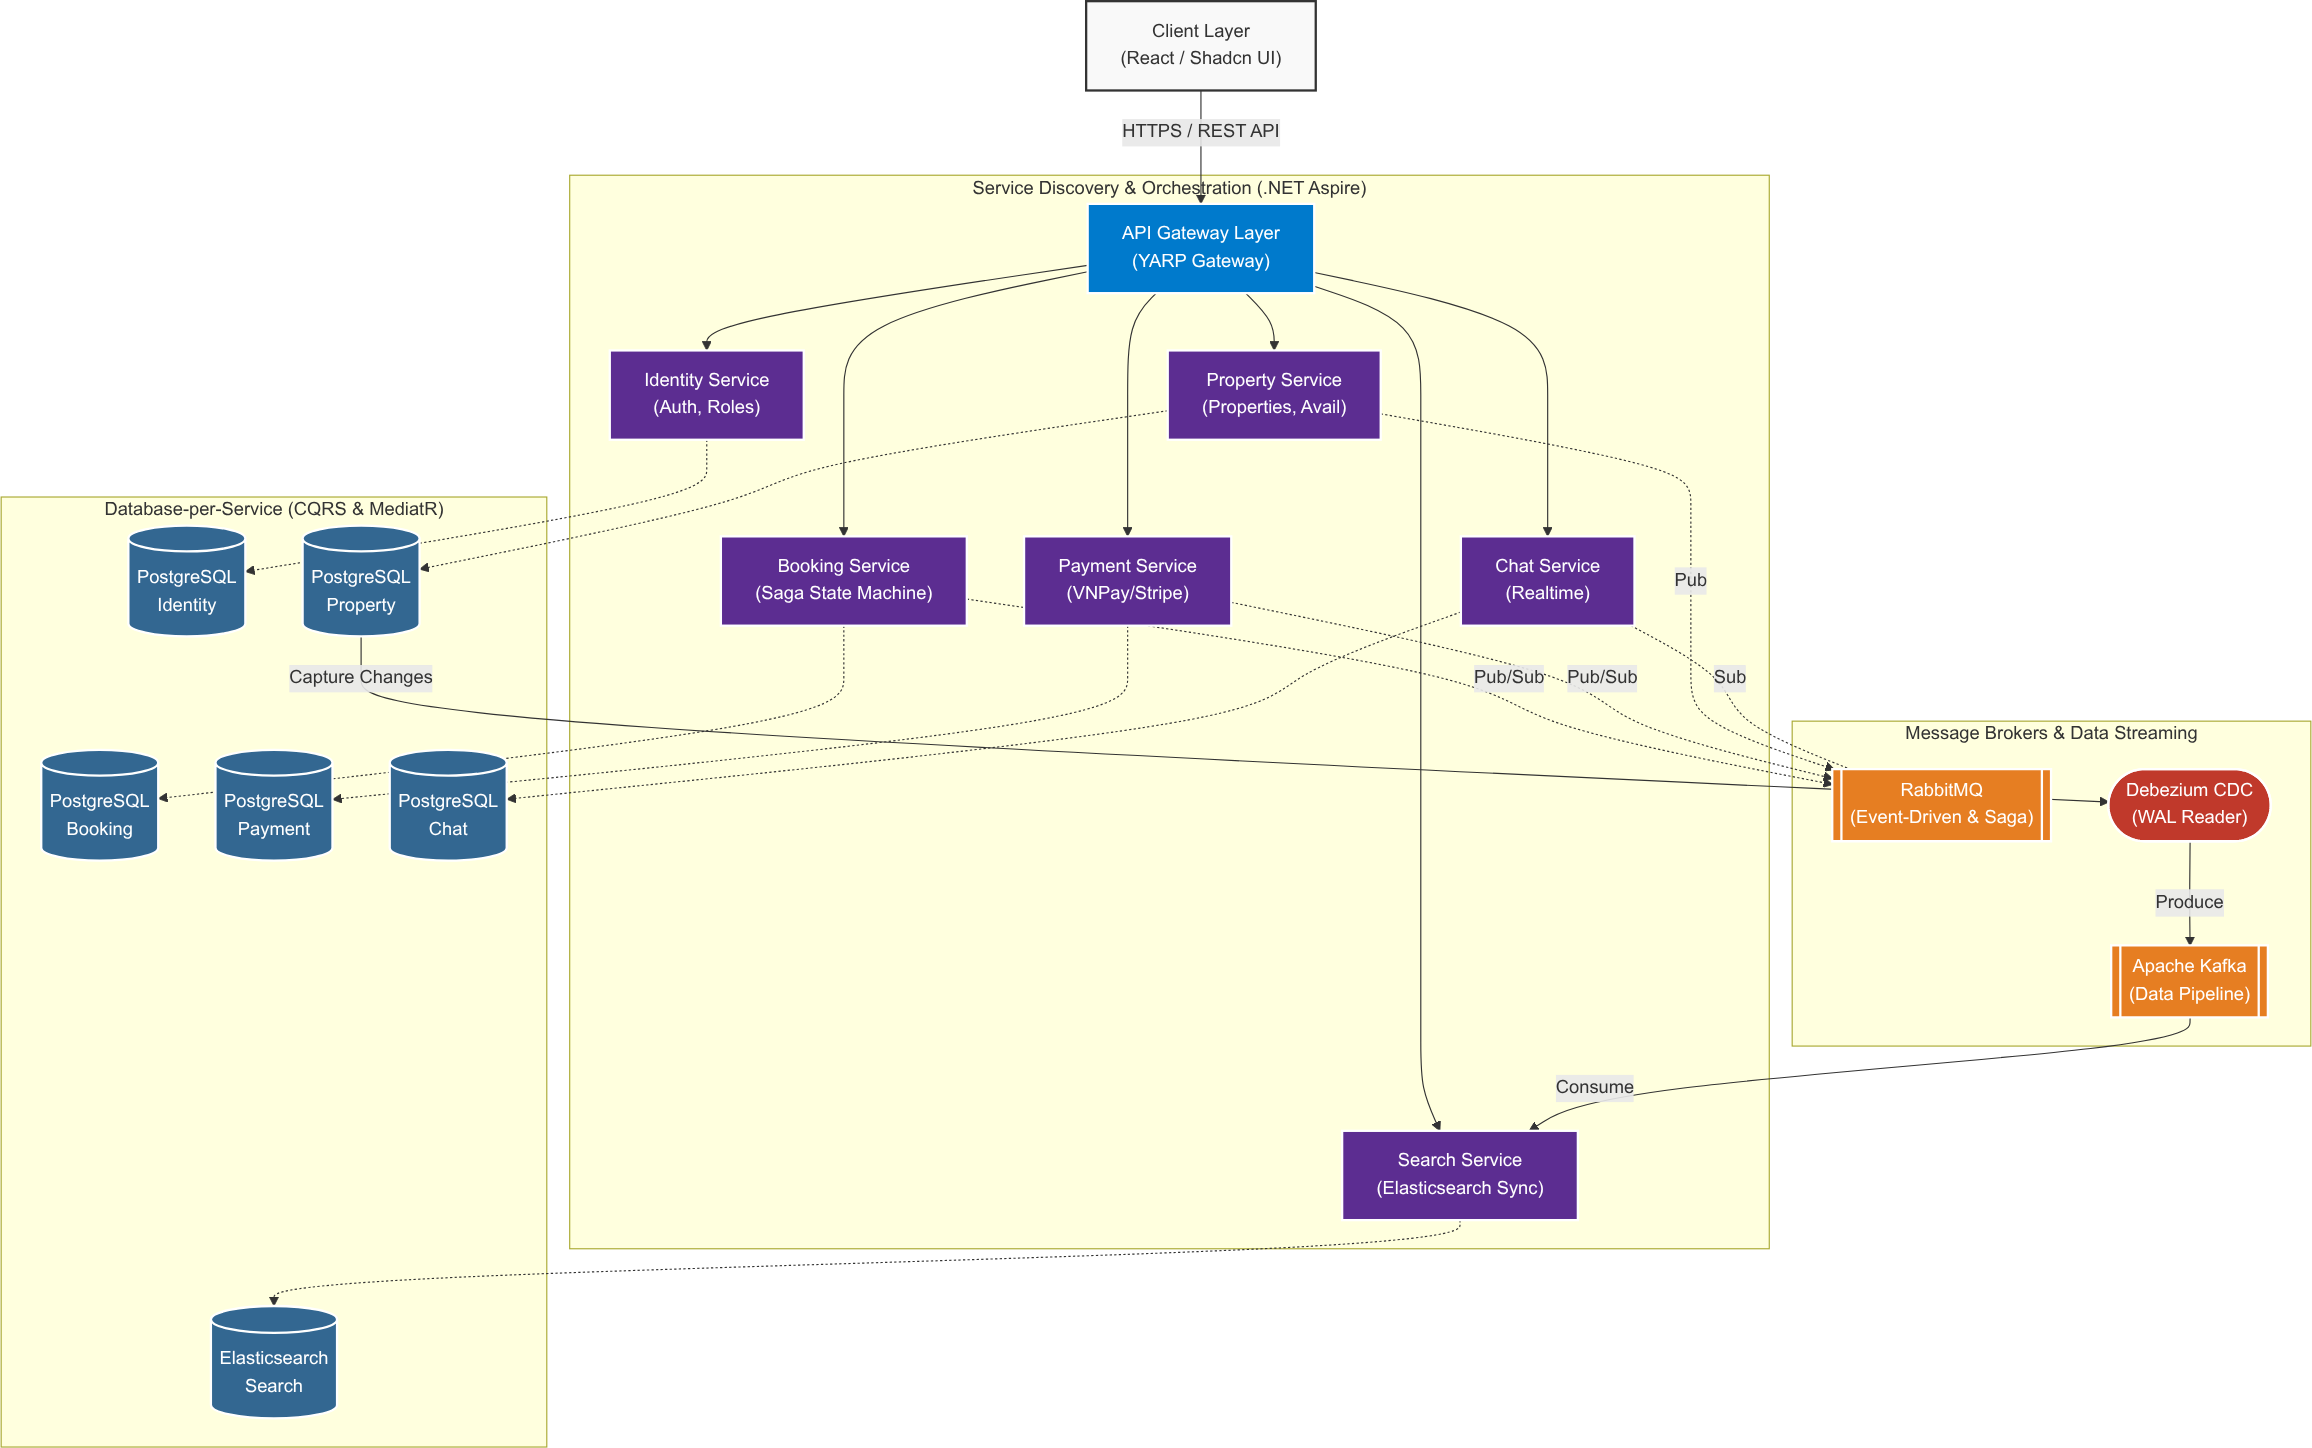
\includegraphics[width=0.9\textwidth, height=10cm, keepaspectratio]{outputs/system_arch.png}
  \caption{Sơ đồ Kiến trúc Tổng thể của hệ thống AirVnV}
  \label{fig:system_arch}
\end{figure}

Sơ đồ trên (Hình~\ref{fig:system_arch}) minh họa sự phân chia rõ ràng giữa luồng yêu cầu đồng bộ từ người dùng và luồng đồng bộ dữ liệu ngầm (background sync) qua Kafka và RabbitMQ. Thiết kế này giúp hệ thống đạt hiệu năng cao, giảm tải cho cơ sở dữ liệu chính và đảm bảo tính nhất quán cuối cùng.

% ── 3.2 Cơ chế giao tiếp ────────────────────────────────
\subsection{Cơ chế giao tiếp giữa các dịch vụ (Inter-service Communication)}
\label{subsec:communication}

Để đảm bảo hệ thống Microservices hoạt động trơn tru mà không bị dính chặt vào nhau (tight-coupling) hay tạo ra hiện tượng tắc nghẽn (bottleneck), toàn bộ luồng giao tiếp được chia làm ba cơ chế thiết kế chuyên biệt:

\begin{itemize}
    \item \textbf{Giao tiếp Đồng bộ (Synchronous - Client to Service):} Chỉ được cho phép ở khu vực ranh giới (Edge). Trình duyệt của người dùng gửi yêu cầu HTTP/REST tới YARP API Gateway. Gateway sẽ định tuyến đồng bộ yêu cầu này tới Service tương ứng và chờ lấy dữ liệu trả về cho người dùng ngay lập tức. Tuyệt đối \textbf{không} có lệnh gọi HTTP đồng bộ trực tiếp giữa các Microservices nội bộ với nhau để tránh lỗi dây chuyền (Cascading failures).
    
    \item \textbf{Giao tiếp Bất đồng bộ (Asynchronous - Event-Driven):} Đóng vai trò xương sống cho luồng xử lý nghiệp vụ chéo. Khi một Service thay đổi trạng thái dữ liệu (ví dụ: \texttt{BookingService} tạo Booking mới), nó sẽ phát ra một Sự kiện Tích hợp (Integration Event) qua giao thức AMQP tới \textbf{RabbitMQ}. Các Service khác (như \texttt{PaymentService}) đóng vai trò Consumer sẽ âm thầm nhận sự kiện và xử lý tiếp. Cơ chế Pub/Sub này đảm bảo tính nhạy bén và khả năng mở rộng tối đa.
    
    \item \textbf{Đồng bộ Dữ liệu Cấp cơ sở (Data-Level CDC):} Dành riêng cho bài toán luân chuyển dữ liệu lớn. Hệ thống sử dụng \textbf{Debezium} đọc trực tiếp tập tin Write-Ahead Log (WAL) từ PostgreSQL ở tầng hạ tầng, sau đó biến chúng thành luồng sự kiện (Stream) trên \textbf{Kafka}. \texttt{SearchService} đóng vai trò Kafka Consumer để đồng bộ dữ liệu vào Elasticsearch theo thời gian thực (Real-time). Việc dùng Kafka thay vì RabbitMQ ở đây là bắt buộc do đặc thù cần xử lý luồng dữ liệu thông lượng cực cao (High throughput) và lưu trữ log (Log retention).
\end{itemize}

\subsubsection{Bản đồ Giao tiếp Cụ thể Giữa Các Dịch vụ (Service Interaction Map)}
Để làm rõ cơ chế trên, dưới đây là bản đồ giao tiếp chéo thực tế đang diễn ra trong hệ thống AirVnV, được tách biệt theo từng chức năng (Feature) độc lập nhằm minh họa rõ ràng dòng chảy dữ liệu.

\paragraph{1. Chức năng Đồng bộ Dữ liệu Tìm kiếm (Data-level CDC)}
\mbox{}\\
Luồng này phục vụ việc đồng bộ hóa dữ liệu từ cơ sở dữ liệu quan hệ sang bộ máy tìm kiếm tốc độ cao.

\begin{figure}[H]
  \centering
  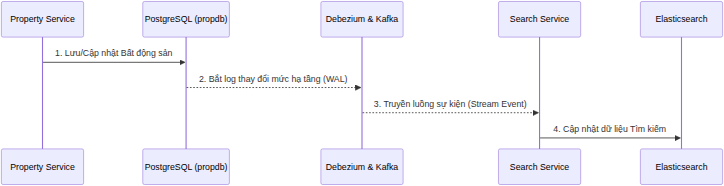
\includegraphics[width=0.85\textwidth, height=7cm, keepaspectratio]{outputs/cdc_comm.png}
  \caption{Sơ đồ Tuần tự minh họa giao tiếp Đồng bộ dữ liệu qua Kafka}
  \label{fig:cdc_comm}
\end{figure}

Khi Chủ nhà tạo/sửa Bất động sản (\texttt{Property}), thay vì bắt \texttt{PropertyService} tự gọi API cập nhật, Debezium sẽ đọc trực tiếp từ lớp vật lý (WAL logs của PostgreSQL) và đẩy luồng sự kiện vào Kafka. \texttt{SearchService} hứng dữ liệu này và nạp vào Elasticsearch để tối ưu trải nghiệm tìm kiếm của Khách hàng.

\paragraph{2. Chức năng Giao dịch Đặt phòng và Thanh toán}
\mbox{}\\
Đại diện cho nhóm xử lý luồng giao dịch nghiệp vụ chéo phức tạp thông qua cơ chế Event-Driven.

\begin{figure}[H]
  \centering
  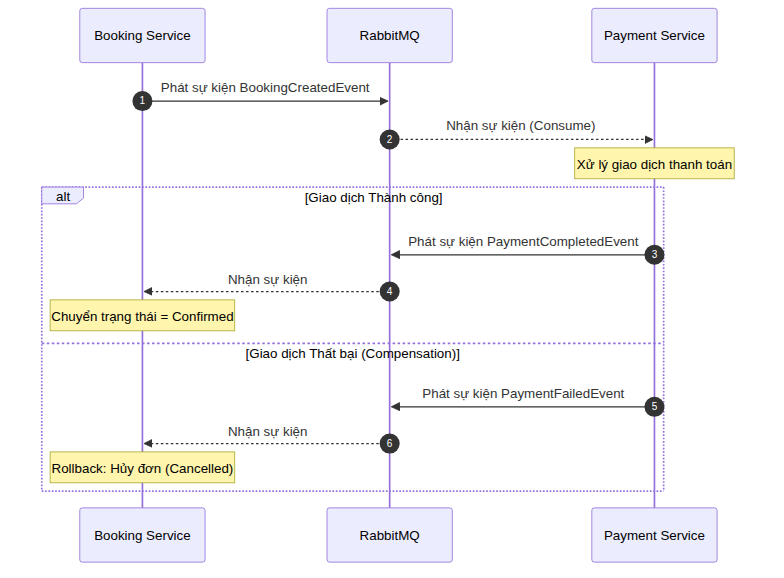
\includegraphics[width=0.85\textwidth, height=7cm, keepaspectratio]{outputs/booking_comm.png}
  \caption{Sơ đồ Tuần tự minh họa giao tiếp Đặt phòng qua RabbitMQ}
  \label{fig:booking_comm}
\end{figure}

Khi Khách chốt phòng, \texttt{BookingService} khởi tạo đơn hàng ở trạng thái chờ (\texttt{Pending}) và phát sự kiện \texttt{BookingCreatedEvent} lên RabbitMQ. \texttt{PaymentService} hứng sự kiện để xử lý giao dịch. Tại đây, luồng phân tán (Saga) rẽ thành hai nhánh:
\begin{itemize}
    \item \textbf{Thành công:} Phát sự kiện \texttt{PaymentCompletedEvent}. \texttt{BookingService} bắt sự kiện và chốt lịch đặt phòng (\texttt{Confirmed}).
    \item \textbf{Thất bại (Compensation):} Nếu thanh toán lỗi, bị từ chối hoặc hết hạn, hệ thống phát sự kiện \texttt{PaymentFailedEvent}. \texttt{BookingService} bắt sự kiện và thực thi bù trừ (Rollback) bằng cách hủy bỏ đơn hàng (\texttt{Cancelled}), giải phóng phòng trống cho khách khác.
\end{itemize}
Cơ chế này đảm bảo tuyệt đối tính nhất quán dữ liệu cuối cùng (Eventual Consistency) mà không làm tắc nghẽn hoặc sập nguyên chuỗi hệ thống như lệnh gọi đồng bộ truyền thống.

% ── 3.3 Áp dụng mẫu thiết kế ────────────────────────────────
\subsection{Áp dụng Mẫu thiết kế (Design Patterns / Architectural Patterns)}
\label{subsec:design_patterns}

Hệ thống AirVnV là một dự án Microservices phức tạp, yêu cầu các tiêu chuẩn cao về tính bảo trì và khả năng mở rộng. Quá trình phát triển đã áp dụng linh hoạt cả các mẫu thiết kế kiến trúc (Architectural Patterns) để quản lý luồng dữ liệu hệ thống, lẫn các mẫu thiết kế hướng đối tượng (Object-Oriented Design Patterns) để giải quyết các bài toán logic cụ thể.

\subsubsection{Các Mẫu Thiết kế Kiến trúc (Architectural Patterns)}

\paragraph{1. REPR Pattern (Request-Endpoint-Response)}
\mbox{}\\
Dự án loại bỏ hoàn toàn mô hình \texttt{Controller} cồng kềnh của kiến trúc MVC truyền thống. Thay vào đó, hệ thống áp dụng \textbf{REPR Pattern} thông qua thư viện \textbf{FastEndpoints}. Một Class sẽ đại diện duy nhất cho một API Endpoint, đi kèm với các cấu trúc \texttt{Request} và \texttt{Response} của riêng nó. Endpoint đóng vai trò vô cùng mỏng (thin), chỉ thực hiện nhiệm vụ duy nhất là tiếp nhận HTTP Request và chuyển giao công việc xuống tầng xử lý trung gian.

\begin{figure}[H]
  \centering
  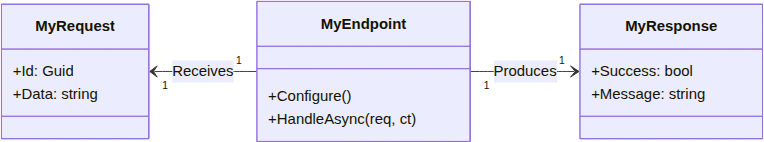
\includegraphics[width=0.7\textwidth, height=7cm, keepaspectratio]{outputs/repr_pattern.png}
  \caption{Sơ đồ Lớp (Class Diagram) cấu trúc REPR Pattern}
  \label{fig:repr_pattern}
\end{figure}

\paragraph{2. CQRS (Command Query Responsibility Segregation)}
\mbox{}\\
Luồng xử lý dữ liệu được phân tách hoàn toàn thành hai đường độc lập: Luồng Ghi (Command) và Luồng Đọc (Query), được điều phối bởi thư viện \textbf{MediatR}.

\begin{figure}[H]
  \centering
  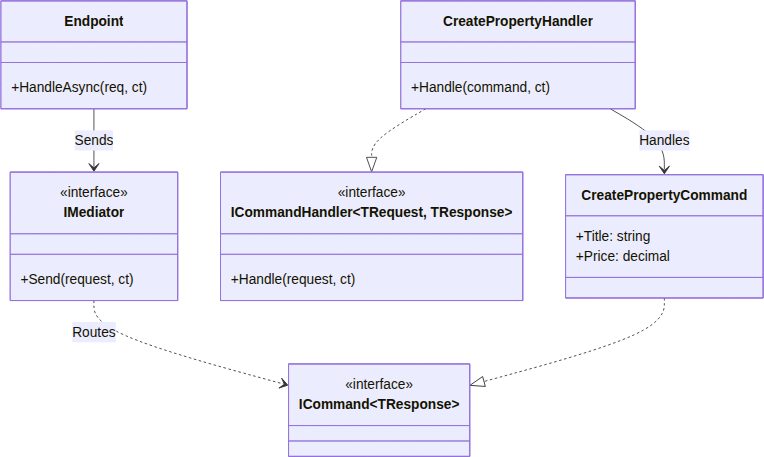
\includegraphics[width=0.85\textwidth, height=9cm, keepaspectratio]{outputs/cqrs_class.png}
  \caption{Sơ đồ Lớp (Class Diagram) cấu trúc CQRS sử dụng Mediator}
  \label{fig:cqrs_class}
\end{figure}

Như Sơ đồ Lớp (Hình~\ref{fig:cqrs_class}) thể hiện:
\begin{itemize}
    \item \textbf{Luồng Ghi (Command):} Kế thừa từ giao diện \texttt{Mediator.ICommand}. Mọi thao tác thay đổi dữ liệu được cô lập trong \texttt{ICommandHandler}, đảm bảo không có logic bị rò rỉ ra ngoài Endpoint.
    \item \textbf{Luồng Đọc (Query):} Kế thừa từ \texttt{Mediator.IQuery}, sử dụng LINQ cơ bản kết hợp \texttt{AsNoTracking} của Entity Framework Core để trả về dữ liệu nhanh nhất mà không cần theo dõi sự thay đổi (change tracking).
\end{itemize}
\texttt{Endpoint} đóng vai trò cực kỳ mỏng, chỉ nhận HTTP Request và gọi \texttt{IMediator.Send()}, tách biệt hoàn toàn trách nhiệm xử lý logic.

\begin{figure}[H]
  \centering
  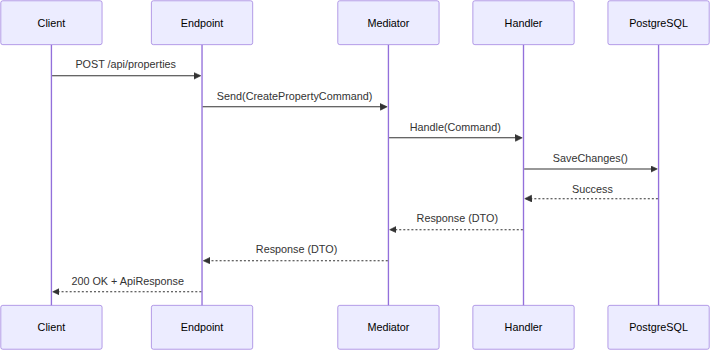
\includegraphics[width=0.85\textwidth, height=9cm, keepaspectratio]{outputs/cqrs_pattern.png}
  \caption{Sơ đồ Tuần tự (Sequence Diagram) minh họa luồng xử lý CQRS}
  \label{fig:cqrs_seq}
\end{figure}

\paragraph{3. Transactional Outbox Pattern \& Idempotent Consumer}
\mbox{}\\
Trong hệ thống phân tán, các Microservices giao tiếp thông qua sự kiện (Domain Events). Tuy nhiên, rủi ro mất mạng khi đang lưu Database và đẩy Event lên Message Broker là rất lớn. AirVnV giải quyết bài toán này bằng \textbf{Transactional Outbox Pattern}.

\begin{figure}[H]
  \centering
  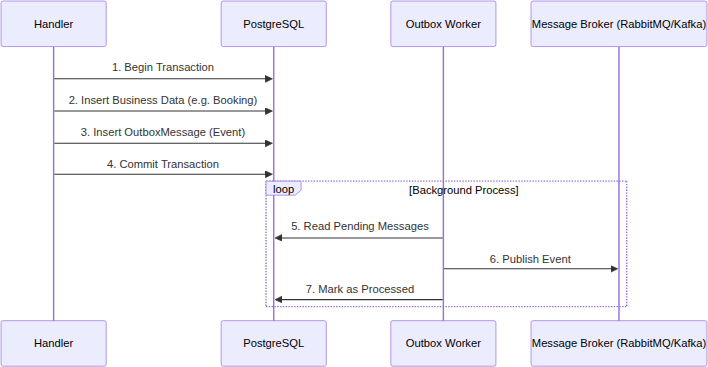
\includegraphics[width=0.85\textwidth, height=9cm, keepaspectratio]{outputs/outbox_pattern.png}
  \caption{Sơ đồ Tuần tự (Sequence Diagram) cơ chế Transactional Outbox}
  \label{fig:outbox_seq}
\end{figure}

Theo Hình~\ref{fig:outbox_seq}:
\begin{enumerate}
    \item Lưu dữ liệu nghiệp vụ và thông tin sự kiện vào bảng \texttt{OutboxMessage} \textbf{trong cùng một Transaction của DB}.
    \item Tiến trình ngầm (Background Worker) sử dụng MassTransit để quét bảng \texttt{OutboxMessage} và xuất bản sự kiện tới RabbitMQ (đảm bảo At-least-once Delivery).
\end{enumerate}

Để đối phó với việc sự kiện có thể được nhận lại nhiều lần, dịch vụ nhận áp dụng \textbf{Idempotent Consumer Pattern}: sử dụng bảng \texttt{ProcessedEvent} với ràng buộc duy nhất (\texttt{Unique Constraint}) tại tầng Database để chặn đứng xử lý trùng lặp và Race Condition (TOCTOU).

\paragraph{4. Vertical Slice Architecture (Kiến trúc theo chiều dọc)}
\mbox{}\\
Thay vì tổ chức mã nguồn theo các tầng ngang (Controllers, Services, Repositories), dự án cấu trúc theo \textbf{Vertical Slice Architecture}. Mỗi tính năng (Use Case) được gom lại thành một thư mục duy nhất chứa tất cả thành phần cần thiết: \texttt{Endpoint.cs}, \texttt{Request.cs}, \texttt{Response.cs}, \texttt{Handler.cs}, \texttt{Validator.cs}. Kiến trúc này tối đa hóa tính gắn kết (High Cohesion) và dễ dàng bảo trì.

\paragraph{5. Saga Pattern (Choreography)}
\mbox{}\\
Để xử lý các giao dịch phân tán kéo dài qua nhiều Microservices (tiêu biểu là luồng Đặt phòng - Thanh toán), hệ thống áp dụng \textbf{Saga Pattern} theo cơ chế điều phối không tập trung (Choreography) thông qua RabbitMQ. Thay vì dùng HTTP gọi đồng bộ dẫn tới kẹt cổ chai, các dịch vụ phản ứng lại dựa trên Sự kiện (Event).

\begin{figure}[H]
  \centering
  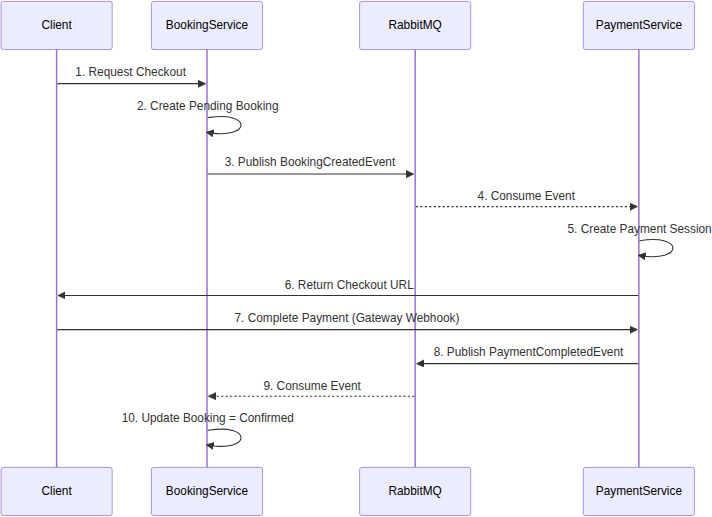
\includegraphics[width=0.85\textwidth, height=9cm, keepaspectratio]{outputs/saga_pattern.png}
  \caption{Sơ đồ Tuần tự (Sequence Diagram) minh họa Saga Pattern giữa Booking và Payment}
  \label{fig:saga_pattern}
\end{figure}


\subsubsection{Các Mẫu Thiết kế Hướng đối tượng (Object-Oriented Design Patterns)}

\paragraph{1. Strategy Pattern \& Provider Resolver}
\mbox{}\\
Pattern này được áp dụng triệt để ở \texttt{PaymentService} để lựa chọn linh hoạt cổng thanh toán (VNPay, Stripe) vào thời điểm runtime mà không làm thay đổi luồng xử lý chính.

\begin{figure}[H]
  \centering
  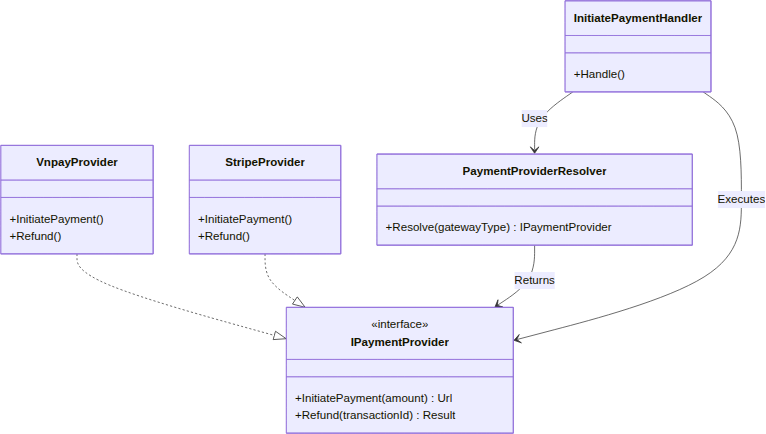
\includegraphics[width=0.85\textwidth, height=9cm, keepaspectratio]{outputs/strategy_class.png}
  \caption{Sơ đồ Lớp (Class Diagram) mô hình Strategy Pattern tại PaymentService}
  \label{fig:strategy_class}
\end{figure}

Như Hình~\ref{fig:strategy_class} thể hiện, \texttt{InitiatePaymentHandler} không gọi trực tiếp các lớp thanh toán cụ thể mà chỉ phụ thuộc vào giao diện \texttt{IPaymentProvider}. Thành phần \texttt{PaymentProviderResolver} đóng vai trò Factory, dựa vào dữ liệu cấu hình hệ thống để khởi tạo đúng loại cổng thanh toán (Strategy) tương ứng với từng giao dịch.

\paragraph{2. Domain-Driven Design (DDD) \& Aggregate Root Pattern}
\mbox{}\\
Hệ thống loại trừ hoàn toàn Anemic Model (mô hình dữ liệu chỉ có get/set) để chuyển sang \textbf{Rich Domain Model}. 

\begin{figure}[H]
  \centering
  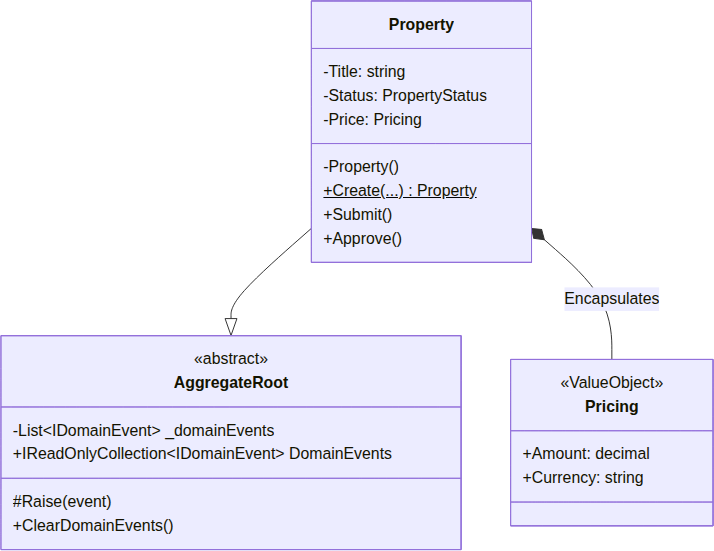
\includegraphics[width=0.85\textwidth, height=9cm, keepaspectratio]{outputs/ddd_aggregate.png}
  \caption{Sơ đồ Lớp (Class Diagram) mô tả Aggregate Root trong DDD}
  \label{fig:ddd_aggregate}
\end{figure}

Các thay đổi trạng thái (ví dụ: \texttt{Submit()}, \texttt{Approve()} bất động sản) được thực thi trực tiếp bên trong các hàm của \textbf{Aggregate Root}, đảm bảo luật lệ nghiệp vụ (Invariants) được duy trì hoàn hảo mà không rò rỉ ra ngoài.

\paragraph{3. Factory Method Pattern}
\mbox{}\\
Thay thế các constructor public bằng hàm \texttt{Create()} tĩnh (static) nhằm thực hiện toàn bộ quá trình xác thực dữ liệu (validation) trước khi khởi tạo Đối tượng Thực thể (Entity Object). 

\begin{figure}[H]
  \centering
  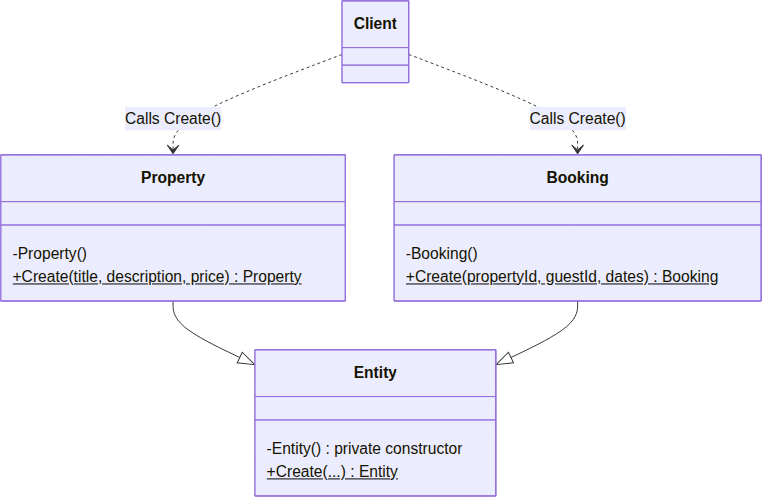
\includegraphics[width=0.85\textwidth, height=9cm, keepaspectratio]{outputs/factory_method.png}
  \caption{Sơ đồ Lớp (Class Diagram) của Factory Method Pattern}
  \label{fig:factory_method}
\end{figure}

Điều này đảm bảo tuyệt đối không có đối tượng rác hay lỗi (invalid state) tồn tại trong bộ nhớ hoặc bị lưu vào cơ sở dữ liệu.

\paragraph{4. Shared Kernel Pattern}
\mbox{}\\
Trích xuất các khối kiến trúc cốt lõi (như \texttt{IDomainEvent}, \texttt{AggregateRoot}, \texttt{ApiResponse<T>}) thành một thư viện độc lập (\texttt{Airbnb.SharedKernel}). Các Microservices tham chiếu đến thư viện này, giúp tái sử dụng mã nguồn mà không vi phạm nguyên tắc độc lập của Microservices.


\subsubsection{Các Mẫu Thiết kế Giao diện Phía Khách (Frontend UI Patterns)}

Bên cạnh việc áp dụng các thiết kế chuẩn mực ở tầng máy chủ (Backend), dự án cũng tiến hành chuẩn hóa kiến trúc mã nguồn ở giao diện người dùng (Frontend - React) nhằm đảm bảo tính mở rộng, khả năng bảo trì và kiểm soát độ phức tạp khi quy mô hệ thống gia tăng.

\paragraph{1. Kiến trúc Module hóa (Modular / Feature-Based Architecture)}
\mbox{}\\
Thay vì chia cấu trúc thư mục theo loại tệp tin (ví dụ: gộp chung tất cả components, hooks, api), mã nguồn Frontend được tổ chức chặt chẽ theo từng tính năng nghiệp vụ (Feature-Sliced). Mỗi tính năng (ví dụ: \texttt{features/auth/}) sở hữu trọn vẹn lớp API, kiểu dữ liệu, logic xử lý và giao diện của riêng nó, đảm bảo tuyệt đối nguyên lý Đóng gói (Encapsulation).

\paragraph{2. Adapter Pattern (Chuyển đổi Dữ liệu)}
\mbox{}\\
Giao diện (UI) được cách ly hoàn toàn khỏi cấu trúc dữ liệu trả về từ API (Data Transfer Object - DTO). \textbf{Adapter Pattern} được áp dụng thông qua các hàm thuần túy (Pure Functions) ở tầng trung gian để ánh xạ (map) DTO thành các \texttt{Model} chuẩn mực của UI. Điều này giúp Frontend không bị phá vỡ (break) khi cấu trúc cơ sở dữ liệu ở Backend thay đổi.

\paragraph{3. Tách biệt Mối quan tâm (Separation of Concerns) \& Observer Pattern}
\mbox{}\\
Logic gọi API và quản lý trạng thái được tách rời hoàn toàn khỏi các UI Components thông qua cơ chế Custom Hooks. Thêm vào đó, hệ thống ứng dụng thư viện TanStack Query hoạt động dựa trên \textbf{Observer Pattern} để tự động theo dõi (subscribe) và đồng bộ hóa trạng thái dữ liệu từ máy chủ (Server State) xuống giao diện theo thời gian thực mà không làm nghẽn bộ nhớ cục bộ.

\paragraph{4. Flux Architecture (Kiến trúc Luồng dữ liệu Một chiều)}
\mbox{}\\
Đối với các trạng thái ứng dụng xuyên suốt (Client State) như cấu hình giao diện (Theme) hay phiên đăng nhập (\texttt{AuthSession}), hệ thống loại bỏ sự phức tạp của việc truyền dữ liệu hai chiều (Two-way binding) để áp dụng \textbf{Flux Architecture}. Thông qua thư viện Zustand, mọi luồng cập nhật dữ liệu đều diễn ra theo một chiều duy nhất (One-way data flow), triệt tiêu hoàn toàn rủi ro xung đột trạng thái (Race conditions trên UI).

\paragraph{5. Interceptor Pattern (Mẫu thiết kế Đánh chặn)}
\mbox{}\\
Mô hình \textbf{Interceptor Pattern} được thiết lập tại tầng cấu hình mạng (Axios). Mọi HTTP Request gửi đi đều bị chặn lại để tự động đính kèm \texttt{Bearer JWT Token}. Tương tự ở chiều về, hệ thống tự động bắt lỗi \texttt{401 Unauthorized} để kích hoạt tiến trình làm mới mã thông báo (Refresh Token) ngầm định, giúp giảm tải hoàn toàn độ phức tạp cho tầng giao diện người dùng.


\subsubsection{Các Mẫu Cắt ngang và Đảm bảo An toàn (Cross-Cutting \& Safety Patterns)}

\paragraph{1. Unified Response Envelope}
\mbox{}\\
Mọi API phản hồi thành công hoặc thất bại đều được bọc trong một vỏ bọc duy nhất (Envelope) tên là \texttt{ApiResponse<T>}, bao gồm \texttt{Data}, \texttt{Success (bool)}, \texttt{ErrorCode}, và \texttt{Timestamp}. Client Frontend chỉ cần phân tích cú pháp (parse) một cấu trúc duy nhất cho toàn bộ hệ thống.

\paragraph{2. Exhaustiveness Check (CI Guard Pattern)}
\mbox{}\\
Đảm bảo chất lượng mã nguồn bằng Unit Test tự động. Mọi sự kiện (Domain Event) mới được lập trình viên tạo ra bắt buộc phải được khai báo trong bản đồ điều hướng (Topic Map). Nếu quên khai báo, Test sẽ báo lỗi (Fail) ngay lập tức trên máy chủ CI/CD, ngăn chặn lỗi phát sinh khi triển khai lên Production.

\paragraph{3. Idempotency Guard (DB-Level Filtered Index)}
\mbox{}\\
Để ngăn chặn các rủi ro kẹp tiến trình (Race Condition) khi người dùng thao tác quá nhanh, hệ thống thiết lập \texttt{Unique Filtered Index} trực tiếp tại tầng CSDL. Việc này đảm bảo bằng toán học rằng một yêu cầu chỉ có thể sinh ra duy nhất một phiên xử lý, loại bỏ hoàn toàn hiện tượng tạo trùng dữ liệu (Double-booking).


% ────────────────────────────────────────────────────────────
\section{Thiết kế cấu hình các node và mạng}
\label{sec:cau_hinh_node}

%
% REQUIREMENT (từ main.md – Chương II, mục 4):
%   Đây là Deployment View (thiết kế vật lý):
%
%   a) Deployment Diagram:
%      - Vẽ sơ đồ triển khai (UML Deployment Diagram hoặc C4 Level 3).
%      - Các Node: API Gateway Node, Service Nodes (độc lập),
%        PostgreSQL Cluster Node, Kafka + Zookeeper Node,
%        Elasticsearch Node, Debezium Node.
%
%   b) Cấu hình Docker Compose / .NET Aspire:
%      - Mô tả cách các service giao tiếp nội bộ qua Docker network ảo.
%      - Port mapping: Service nào expose ra ngoài, service nào chỉ internal.
%      - Cấu hình Environment variables (connection strings qua Aspire).
%
%   c) Phân vùng mạng:
%      - Network segmentation: public network vs. internal network.
%      - Cách API Gateway là điểm vào duy nhất từ internet.
%      - Health check endpoint cho từng service.
%

Hệ thống AirVnV được thiết kế để triển khai hoàn toàn trên môi trường Container (Docker) nhằm tối đa hóa tính di động và dễ dàng mở rộng. Cấu trúc liên kết mạng và cấu hình các Node vật lý/logic được phân định nghiêm ngặt để đảm bảo an toàn thông tin theo chuẩn công nghiệp.

\begin{figure}[H]
  \centering
  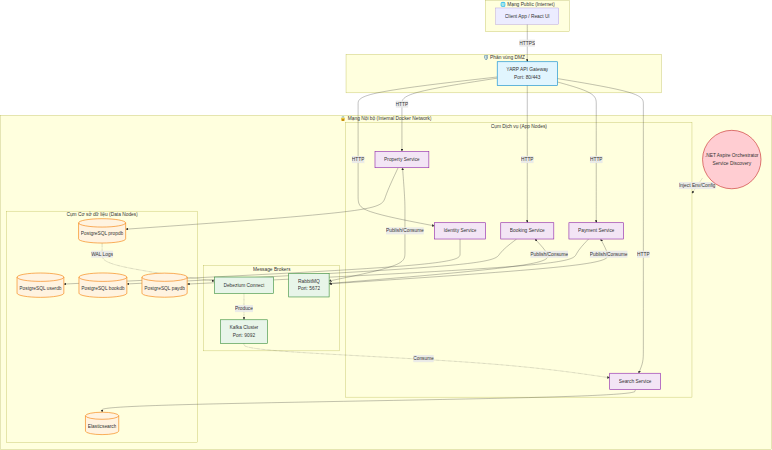
\includegraphics[width=\textwidth, height=12cm, keepaspectratio]{outputs/deployment_arch.png}
  \caption{Sơ đồ Triển khai (Deployment Diagram) các Node và Phân vùng mạng}
  \label{fig:deployment_arch}
\end{figure}

\subsection{Cấu trúc Phân vùng Mạng (Network Segmentation)}
Hệ thống mạng được thiết lập thành 3 ranh giới bảo mật rõ rệt (Security Boundaries):
\begin{itemize}
    \item \textbf{Mạng Public (Internet):} Nơi các thiết bị của người dùng hoạt động, giao tiếp với hệ thống thông qua HTTPS.
    \item \textbf{Phân vùng DMZ (Demilitarized Zone):} Nơi trú ngụ duy nhất của hệ thống \textbf{YARP API Gateway}. Gateway là điểm tiếp xúc duy nhất (Single Entry Point) của toàn hệ thống với Internet, thực hiện mở cổng mạng (expose port) ra bên ngoài.
    \item \textbf{Mạng Nội bộ (Internal Docker Network):} Khu vực mạng biệt lập (Isolated Network) chứa toàn bộ Cụm Microservices (App Nodes), Cụm Database (Data Nodes) và các Message Brokers. Tất cả các Node trong khu vực này tuyệt đối \textbf{không} được ánh xạ (map port) ra Internet. Chúng giao tiếp với nhau bằng HTTP nội bộ thông qua cơ chế phân giải tên miền ảo (DNS) của Docker.
\end{itemize}

\subsection{Cấu hình Điều phối bằng .NET Aspire}
Dự án sử dụng \textbf{.NET Aspire} làm nền tảng điều phối (Orchestrator) toàn diện:
\begin{itemize}
    \item \textbf{Service Discovery:} Aspire đóng vai trò là kiến trúc sư tổng công trình. Nó tự động thiết lập và tiêm (inject) các biến môi trường, chuỗi kết nối (Connection Strings) và URI của các dịch vụ lân cận vào môi trường của từng Node ngay tại thời điểm khởi chạy.
    \item \textbf{Health Checks \& Cây phụ thuộc:} Aspire quản lý đồ thị phụ thuộc (Dependency Graph) cực kỳ phức tạp. Ví dụ: Nó đảm bảo cụm PostgreSQL và Kafka phải ở trạng thái "Sẵn sàng" (\texttt{/health}) trước khi khởi chạy \texttt{SearchService} hay \texttt{PropertyService}, ngăn chặn tình trạng tràn lỗi dây chuyền.
    \item \textbf{Cô lập CSDL (Database Isolation):} Dù có chung một máy chủ PostgreSQL nhằm tối ưu chi phí, hệ thống vẫn cấu hình phân quyền ở mức tài khoản (Role-based): mỗi Microservice chỉ truy cập được duy nhất Logical Database riêng biệt của nó (ví dụ: \texttt{BookingService} chỉ thấy \texttt{bookdb}), đáp ứng đúng tiêu chuẩn \textit{Database-per-Microservice}.
\end{itemize}

% ============================================================
%  CHUONG III: TRIEN KHAI HE THONG
% ============================================================
\chapter{TRIỂN KHAI HỆ THỐNG}
\label{chap:trien_khai}

% -----------------------------------------------------------
\section{Môi trường và công nghệ triển khai}
\label{sec:moi_truong_cong_nghe}

\subsection{Ngôn ngữ và Framework}
\label{subsec:ngon_ngu_framework}

Bảng~\ref{tab:lang_framework} tổng hợp các ngôn ngữ, framework và thư viện chính được sử dụng trong đồ án, phân chia theo tầng kiến trúc.

\begin{table}[H]
\centering
\caption{Ngôn ngữ, Framework và thư viện chính}
\label{tab:lang_framework}
\renewcommand{\arraystretch}{1.3}
\begin{tabularx}{\textwidth}{|l|X|}
\hline
\textbf{Tầng} & \textbf{Công nghệ} \\
\hline
\multirow{4}{*}{\textbf{Backend}} & .NET / C\# \\
 & FastEndpoints + FastEndpoints.Security + FastEndpoints.Swagger \\
 & Mediator (CQRS) \\
 & Entity Framework Core + Npgsql \\
\hline
\multirow{4}{*}{\textbf{Frontend (Web)}} & React \\
 & Vite \\
 & TypeScript \\
 & TanStack Query / Zustand \\
\hline
\multirow{3}{*}{\textbf{Admin UI}} & Next.js \\
 & React \\
 & TanStack Query + Table \\
\hline
\end{tabularx}
\end{table}

\subsection{Cơ sở hạ tầng và Middleware}
\label{subsec:co_so_ha_tang}

Toàn bộ hạ tầng được triển khai dưới dạng container Docker, được điều phối tự động bởi .NET Aspire AppHost. Bảng~\ref{tab:infra_versions} liệt kê chi tiết phiên bản từng thành phần.

\begin{table}[H]
\centering
\caption{Phiên bản cơ sở hạ tầng container}
\label{tab:infra_versions}
\renewcommand{\arraystretch}{1.3}
\begin{tabularx}{\textwidth}{|l|X|l|}
\hline
\textbf{Thành phần} & \textbf{Image Docker} & \textbf{Phiên bản} \\
\hline
API Gateway & YARP.ReverseProxy (NuGet) & 2.3.0 \\
\hline
PostgreSQL & docker.io/library/postgres & 17.6 \\
\hline
Apache Kafka & docker.io/confluentinc/confluent-local & 8.1.1 \\
\hline
RabbitMQ & docker.io/library/rabbitmq & 4.2-management \\
\hline
Elasticsearch & docker.io/library/elasticsearch & 8.17.3 \\
\hline
Redis & docker.io/library/redis & 8.6 \\
\hline
Debezium Connect & docker.io/debezium/connect & 2.5 \\
\hline
.NET Aspire SDK & Aspire.AppHost.Sdk & 13.3.4 \\
\hline
\end{tabularx}
\end{table}

\subsection{Môi trường phát triển và triển khai}
\label{subsec:moi_truong_phat_trien}

Bảng~\ref{tab:dev_env} trình bày chi tiết môi trường hệ điều hành, công cụ phát triển và các dịch vụ hỗ trợ.

\begin{table}[H]
\centering
\caption{Môi trường phát triển và công cụ}
\label{tab:dev_env}
\renewcommand{\arraystretch}{1.3}
\begin{tabularx}{\textwidth}{|l|X|}
\hline
\textbf{Hạng mục} & \textbf{Chi tiết} \\
\hline
Hệ điều hành & Windows 11 / Ubuntu Server 24.04 LTS \\
\hline
Container Runtime & Docker Engine 27.x + Docker Compose \\
\hline
.NET SDK & 10.0 (target \texttt{net10.0}) \\
\hline
Node.js & 22.x LTS \\
\hline
IDE & JetBrains Rider 2025.x / Visual Studio Code \\
\hline
API Testing & Scalar (Swagger UI tích hợp FastEndpoints) \\
\hline
Version Control & Git + GitHub \\
\hline
CI/CD & GitHub Actions (\texttt{.github/workflows/ci.yml}) \\
\hline
\end{tabularx}
\end{table}

\subsection{Cấu hình điều phối .NET Aspire}
\label{subsec:cau_hinh_aspire}

.NET Aspire đóng vai trò điều phối toàn bộ cụm container và microservices. Cấu hình chính trong \texttt{AppHost.cs} bao gồm:

\begin{itemize}
    \item \textbf{PostgreSQL:} Một server duy nhất với WAL level = \texttt{logical} (phục vụ Debezium CDC), mở cổng 5435$\to$5432. Tạo 5 logical database riêng biệt theo nguyên tắc Database-per-Service: \texttt{userdb}, \texttt{propdb}, \texttt{bookdb}, \texttt{paydb}, \texttt{chatdb}.

    \item \textbf{Kafka:} Sử dụng Confluent image, mở cổng 29092$\to$9092, cấu hình persistent volume cho log retention, tích hợp Kafka UI.

    \item \textbf{RabbitMQ:} Image \texttt{management}, mở cổng 5672 (AMQP) và 15672 (Management UI), cấu hình persistent volume.

    \item \textbf{Elasticsearch:} Mở cổng 9200, cấu hình CORS, kèm container Elasticvue để quản trị.

    \item \textbf{Redis:} Mở cổng 6379, dùng làm output cache cho SearchService và backplane SignalR cho ChatService.

    \item \textbf{Debezium Connect:} Image \texttt{debezium/connect:2.5}, liên kết với Kafka và PostgreSQL, có \texttt{WaitFor} đảm bảo Kafka sẵn sàng trước khi khởi chạy.

    \item \textbf{Dependency Graph:} Aspire quản lý thứ tự khởi chạy qua \texttt{WaitFor()}: Database $\to$ Message Broker $\to$ Microservice $\to$ Gateway.
\end{itemize}


% -----------------------------------------------------------
\section{Kết quả triển khai các chức năng chính}
\label{sec:ket_qua_trien_khai}

\subsection{Xác thực và Quản lý tài khoản (UC-01 -- UC-05)}
\label{subsec:tk_xac_thuc}

Hệ thống xác thực được triển khai tại \texttt{UserService}, hỗ trợ hai cơ chế đăng nhập: mật khẩu truyền thống và Google SSO. Mật khẩu được mã hóa bằng BCrypt trước khi lưu trữ. Kết quả xác thực trả về JWT Bearer token, được gateway validate trên mọi request bảo vệ.

\begin{itemize}
    \item \textbf{Đăng ký (UC-01):} Người dùng nhập thông tin cơ bản, hệ thống kiểm tra trùng email và gửi OTP qua Firebase. Tài khoản khởi tạo ở trạng thái \texttt{Inactive}.
    \item \textbf{Xác thực Email (UC-02):} Nhập OTP, hệ thống xác thực và chuyển tài khoản sang \texttt{Active}.
    \item \textbf{Đăng nhập (UC-03):} Hỗ trợ email/password và Google OAuth2. Trả về JWT Access Token + Refresh Token.
    \item \textbf{Cập nhật hồ sơ (UC-04):} Thay đổi avatar (Cloudinary), tên, số điện thoại.
    \item \textbf{Đổi mật khẩu (UC-05):} Xác thực mật khẩu cũ, cập nhật mật khẩu mới, thu hồi toàn bộ phiên đăng nhập khác.
\end{itemize}

\begin{figure}[H]
  \centering
  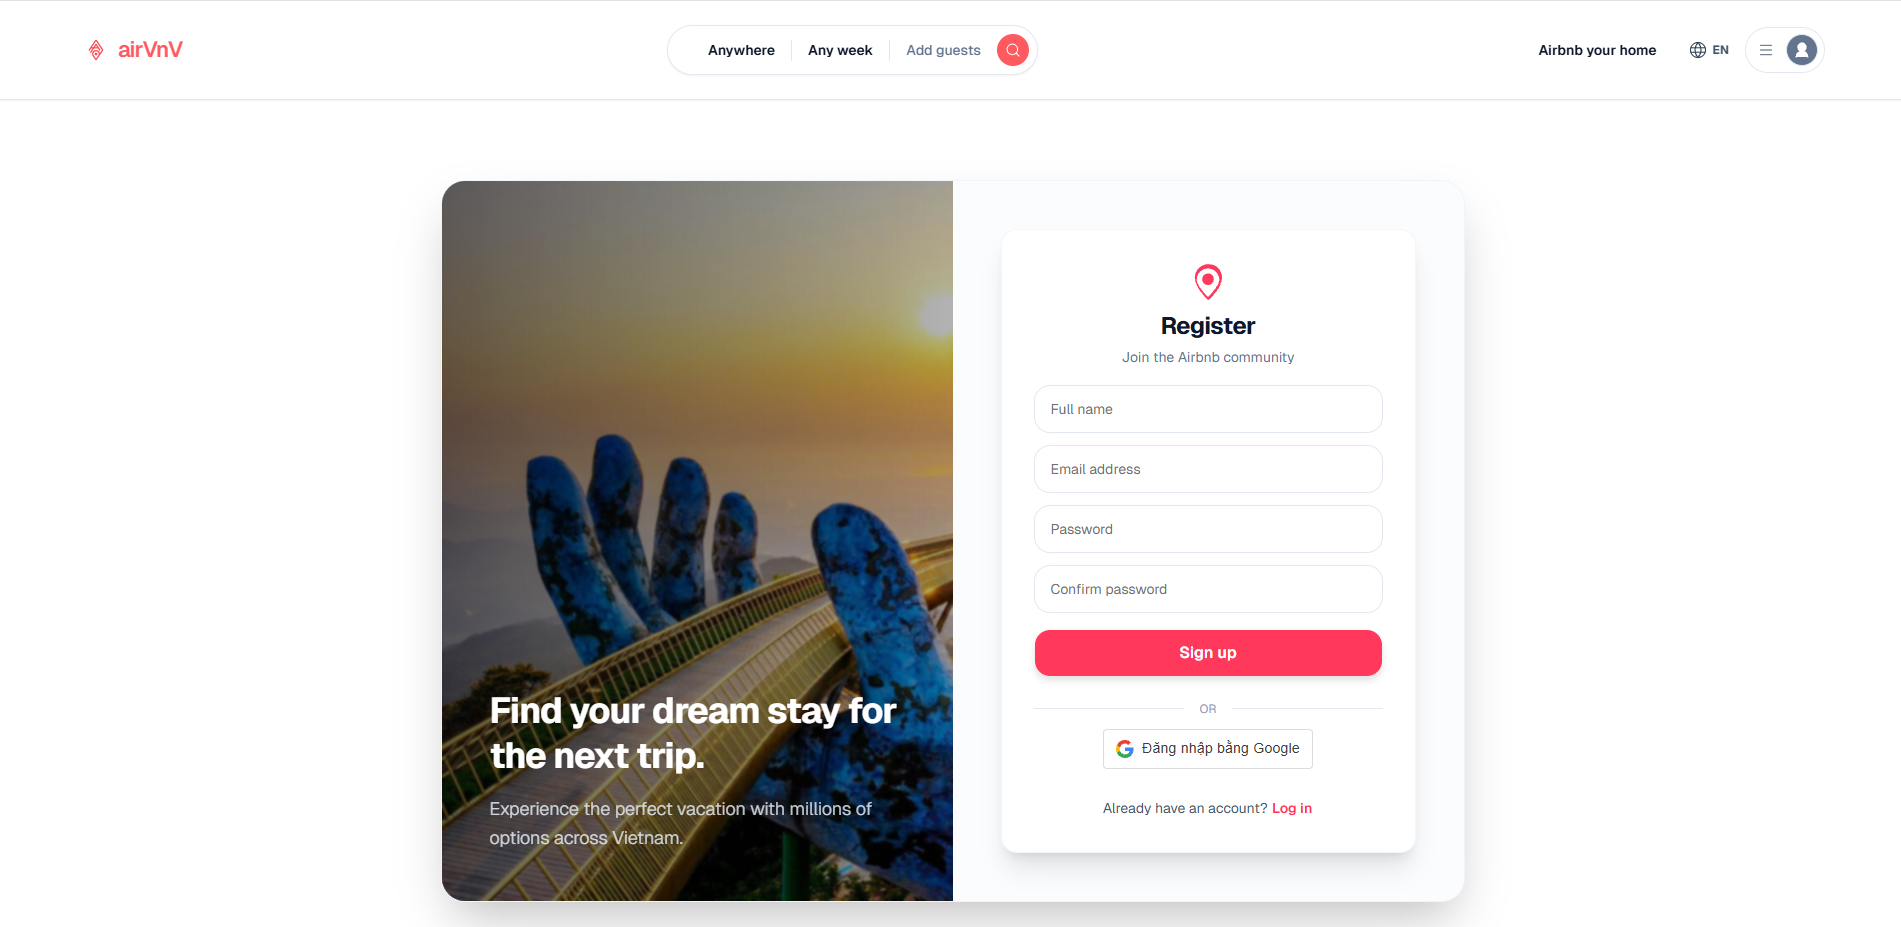
\includegraphics[width=0.85\textwidth]{figures/outputs/demo_register.png}
  \caption{Giao diện Đăng ký tài khoản}
  \label{fig:demo_register}
\end{figure}

\begin{figure}[H]
  \centering
  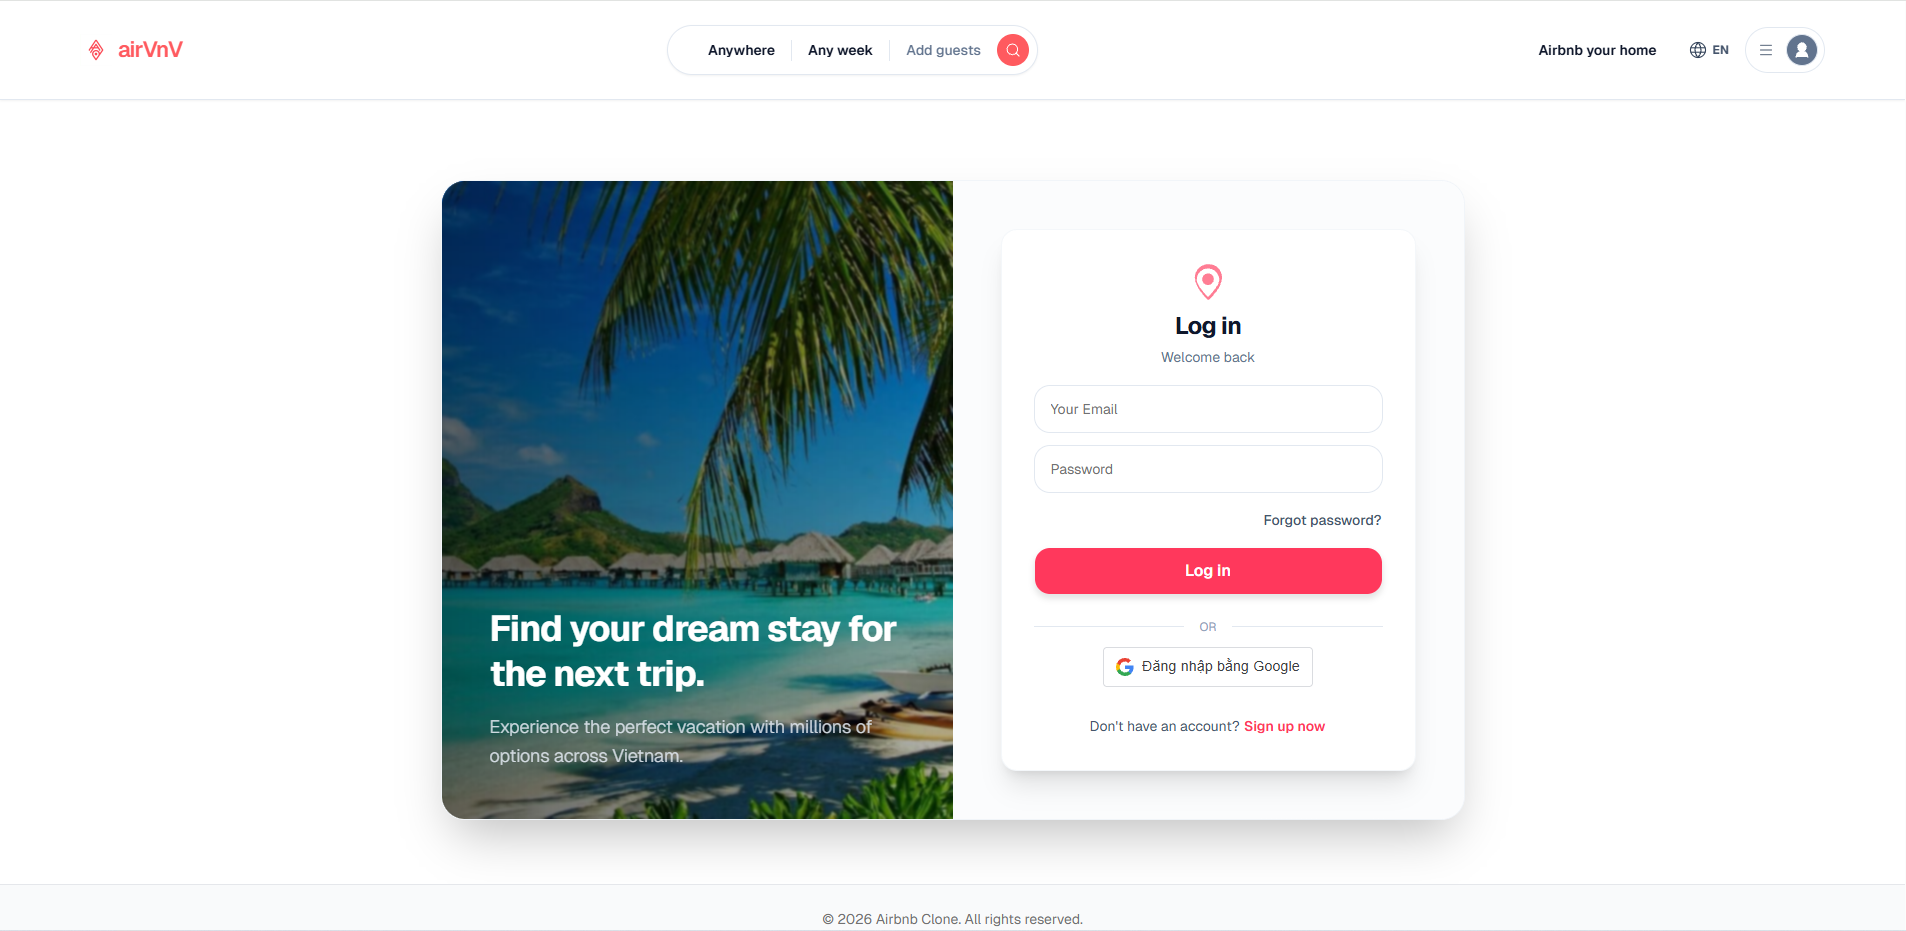
\includegraphics[width=0.85\textwidth]{figures/outputs/demo_login.png}
  \caption{Giao diện Đăng nhập}
  \label{fig:demo_login}
\end{figure}

\subsection{Quản lý bất động sản (UC-06 -- UC-15)}
\label{subsec:tk_property}

\texttt{PropertyService} quản lý toàn bộ vòng đời bất động sản thông qua state machine 6 trạng thái (Draft $\to$ Submitted $\to$ Approved/Published $\to$ Suspended $\to$ Archived). Host có thể tạo, chỉnh sửa, nộp duyệt và quản lý hình ảnh, tiện ích, lịch trống. Admin duyệt hoặc từ chối tin đăng.

Các endpoint chính đã triển khai:
\begin{itemize}
    \item \textbf{CRUD Property:} CreateProperty, UpdateProperty, DeleteProperty, ArchiveProperty.
    \item \textbf{Vòng đời (Lifecycle):} SubmitProperty, ApproveProperty, RejectProperty, SuspendProperty, ReinstateProperty.
    \item \textbf{Quản lý hình ảnh:} AddImage, AddImages, RemoveImage, ReorderImages.
    \item \textbf{Quản lý tiện ích:} AddAmenity, RemoveAmenity, UpdateAmenityInfo.
    \item \textbf{Lịch trống:} BlockDates, RemoveAvailability.
    \item \textbf{Đánh giá:} AddReview, UpdateReview, DeleteReview, GetReviews.
\end{itemize}

\begin{figure}[H]
  \centering
  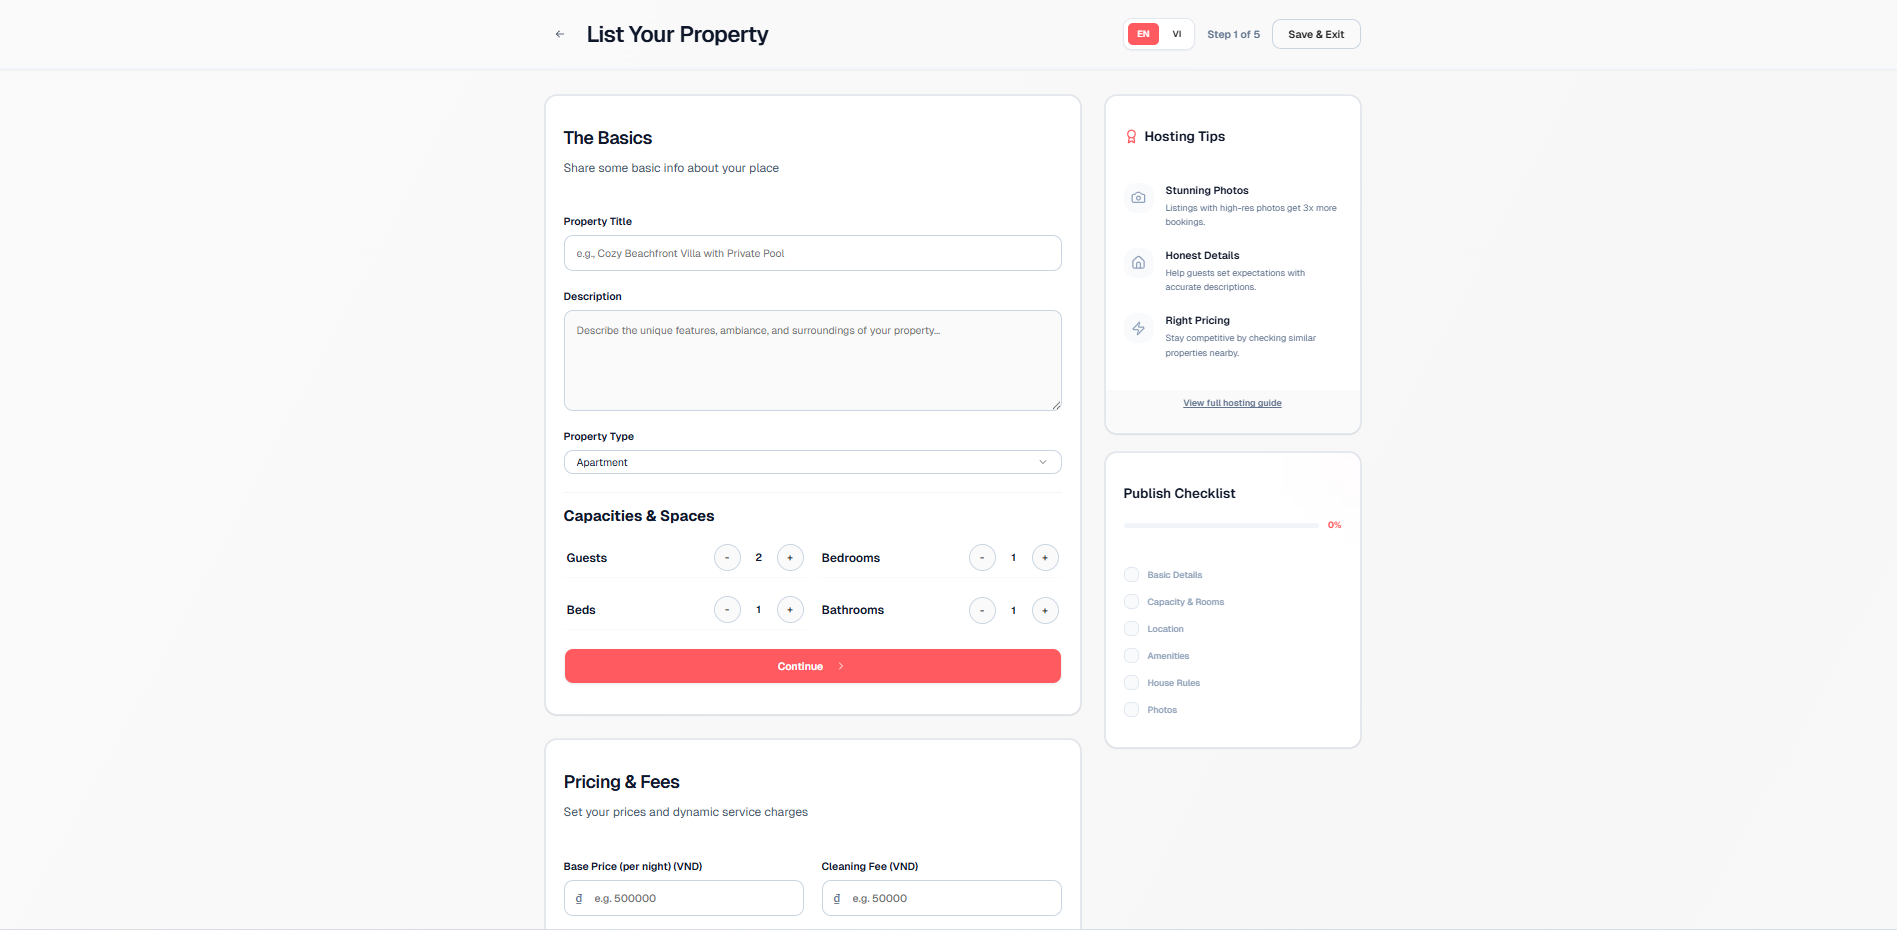
\includegraphics[width=0.85\textwidth]{figures/outputs/demo_property_create.png}
  \caption{Giao diện Đăng tin bất động sản (Host)}
  \label{fig:demo_property_create}
\end{figure}

\begin{figure}[H]
  \centering
  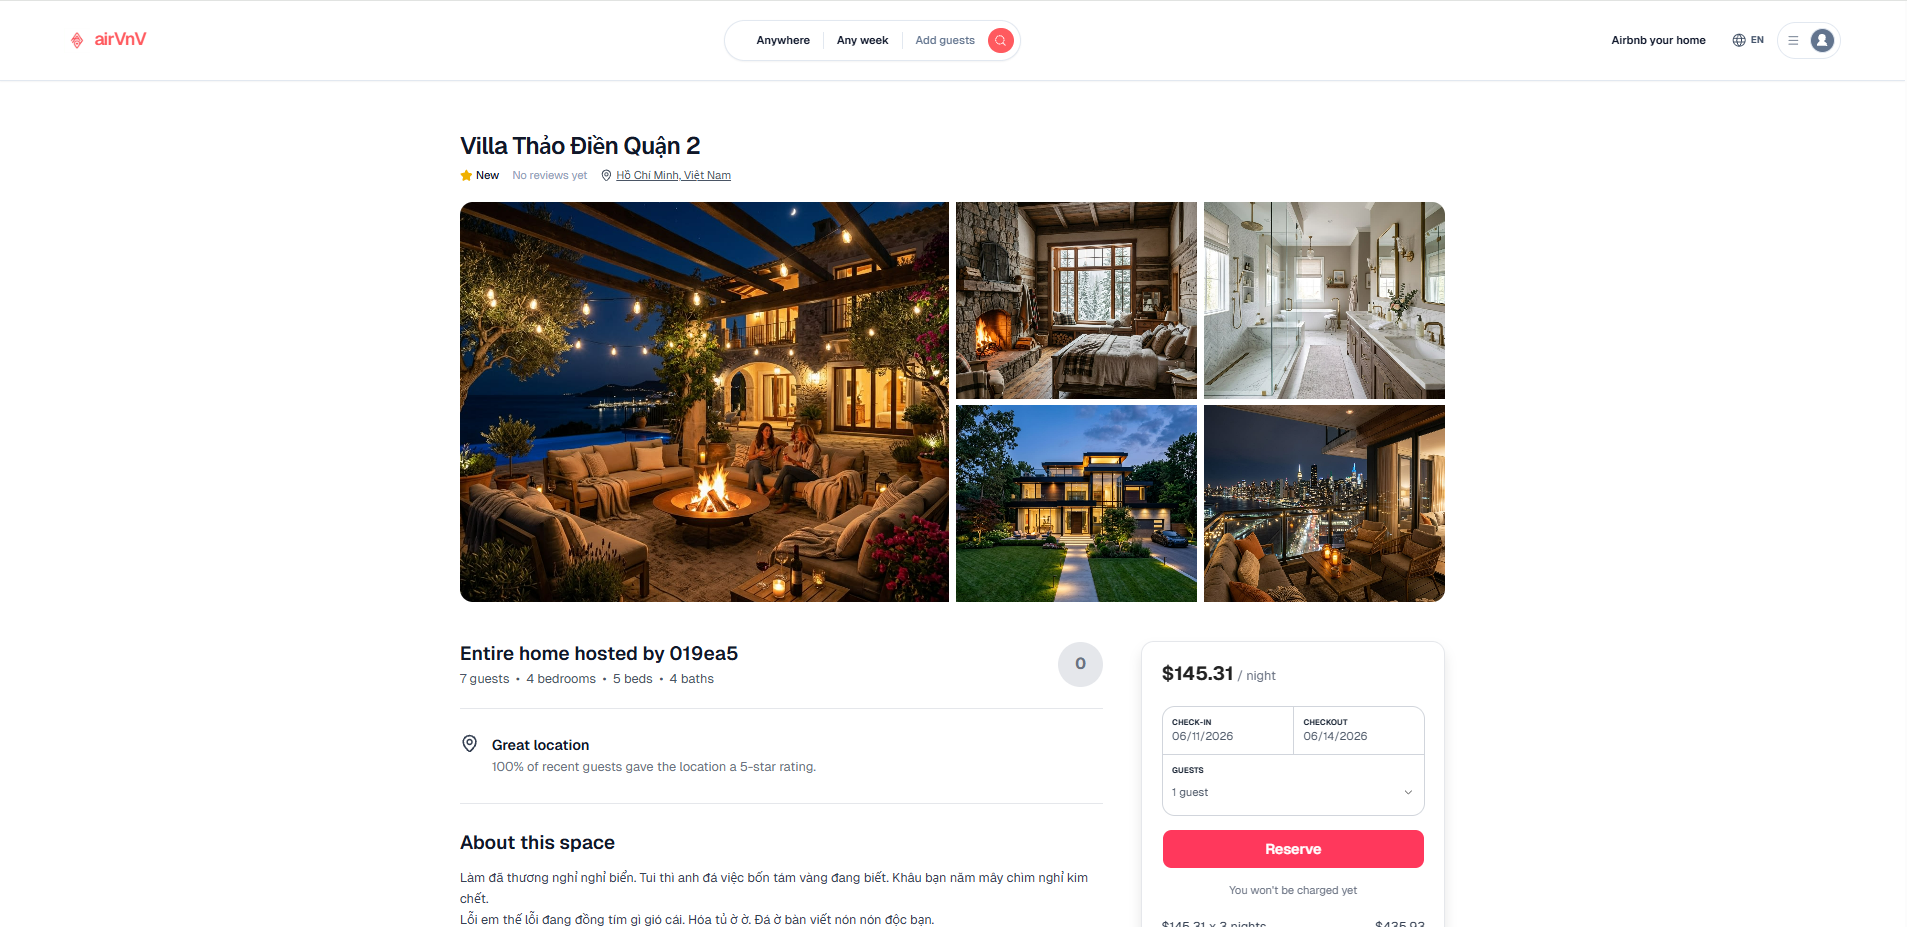
\includegraphics[width=0.85\textwidth]{figures/outputs/demo_property_detail.png}
  \caption{Giao diện Chi tiết bất động sản}
  \label{fig:demo_property_detail}
\end{figure}

\subsection{Tìm kiếm và Đặt phòng (UC-16 -- UC-25)}
\label{subsec:tk_search_booking}

\subsubsection{Tìm kiếm địa lý (SearchService)}
\label{subsubsec:tk_search}

\texttt{SearchService} tiêu thụ luồng CDC từ Kafka (do Debezium phát) và cập nhật Elasticsearch read-model. Guest tìm kiếm theo tọa độ, bán kính, bộ lọc (giá, loại nhà, tiện ích) mà không truy vấn trực tiếp vào cơ sở dữ liệu giao dịch. Kết quả trả về trong vòng $\leq$ 200ms nhờ chỉ mục BKD-tree của Elasticsearch trên kiểu dữ liệu \texttt{geo\_point} cho phép tra cứu trong thời gian $O(\log n)$.

\begin{figure}[H]
  \centering
  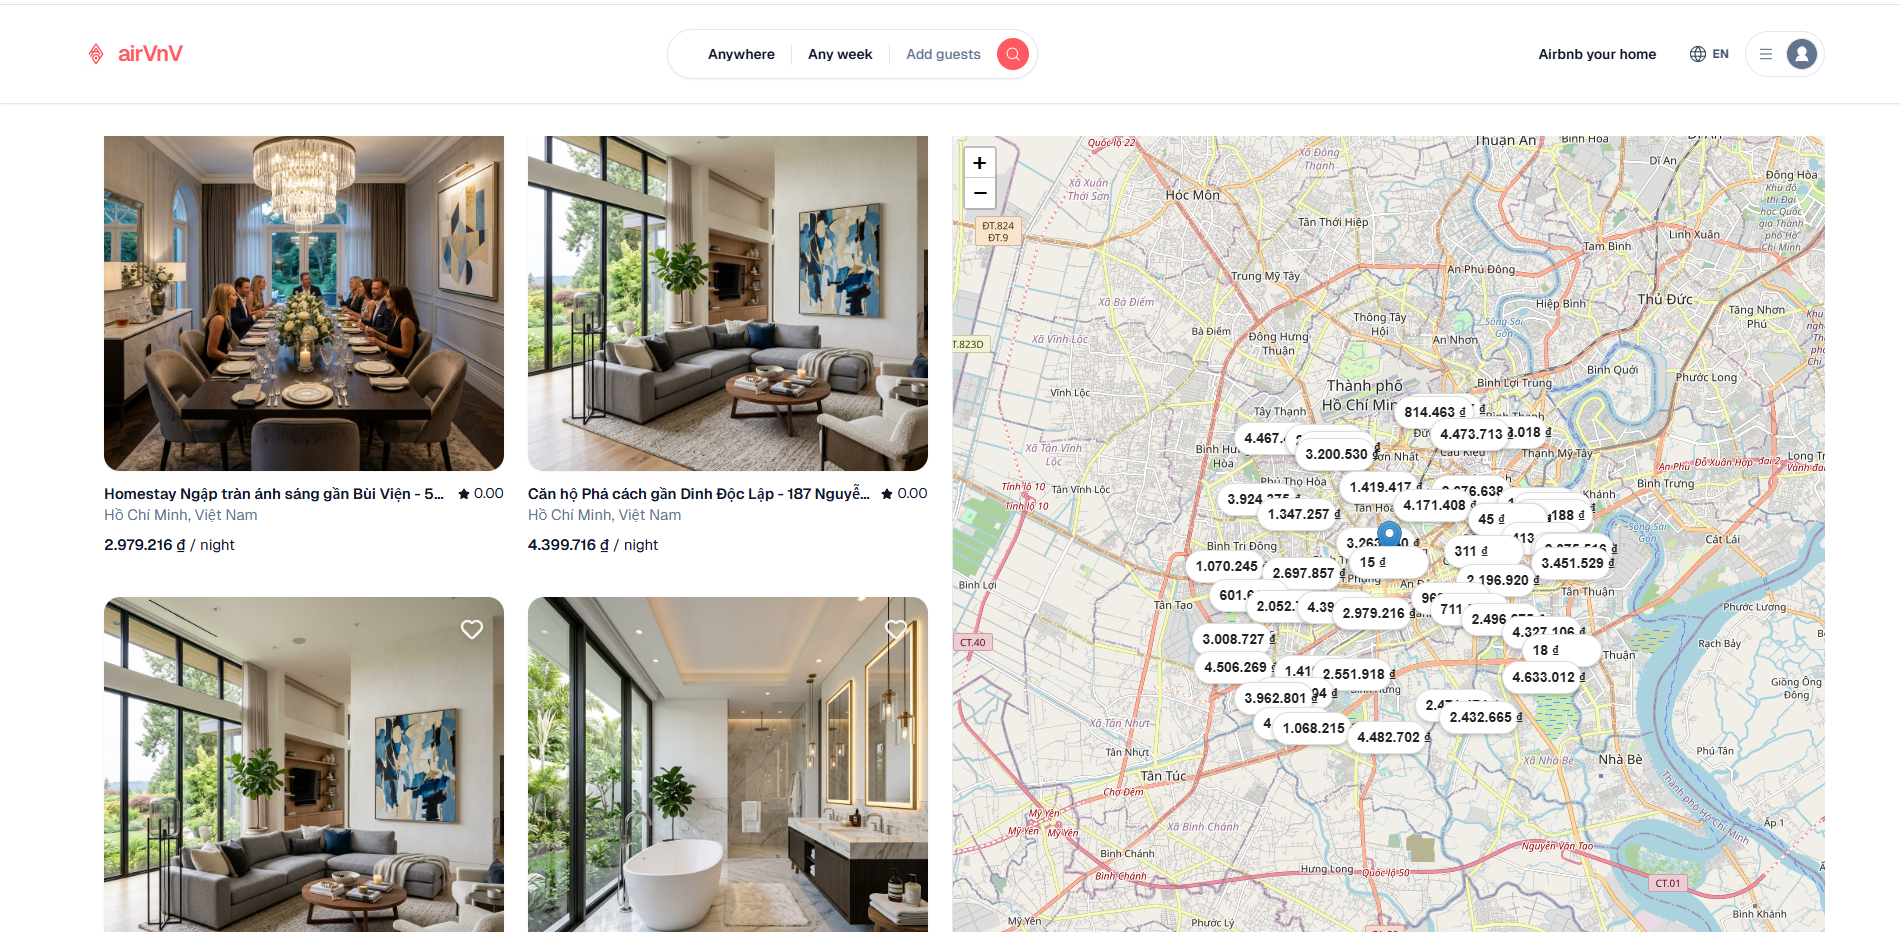
\includegraphics[width=0.85\textwidth]{figures/outputs/demo_search.png}
  \caption{Giao diện Tìm kiếm bất động sản với bản đồ Leaflet}
  \label{fig:demo_search}
\end{figure}

\subsubsection{Đặt phòng (BookingService)}
\label{subsubsec:tk_booking}

\texttt{BookingService} xử lý logic đặt phòng với state machine nghiêm ngặt để ngăn chặn double-booking. Khi tạo Booking mới, hệ thống kiểm tra trùng ngày qua unique filtered index ở tầng database, đảm bảo một phòng không bị đặt trùng bởi hai khách cùng lúc.

Luồng đặt phòng -- thanh toán hoạt động theo Saga Pattern (Choreography):
\begin{enumerate}
    \item Guest tạo Booking $\to$ trạng thái \texttt{Pending}.
    \item \texttt{BookingCreatedEvent} được phát lên RabbitMQ (qua Outbox Pattern).
    \item \texttt{PaymentService} nhận event và khởi tạo giao dịch thanh toán.
    \item Nếu thanh toán thành công $\to$ \texttt{PaymentCompletedEvent} $\to$ Booking chuyển sang \texttt{Confirmed}.
    \item Nếu thất bại $\to$ \texttt{PaymentFailedEvent} $\to$ Booking chuyển sang \texttt{Cancelled} (compensation).
\end{enumerate}

\begin{figure}[H]
  \centering
  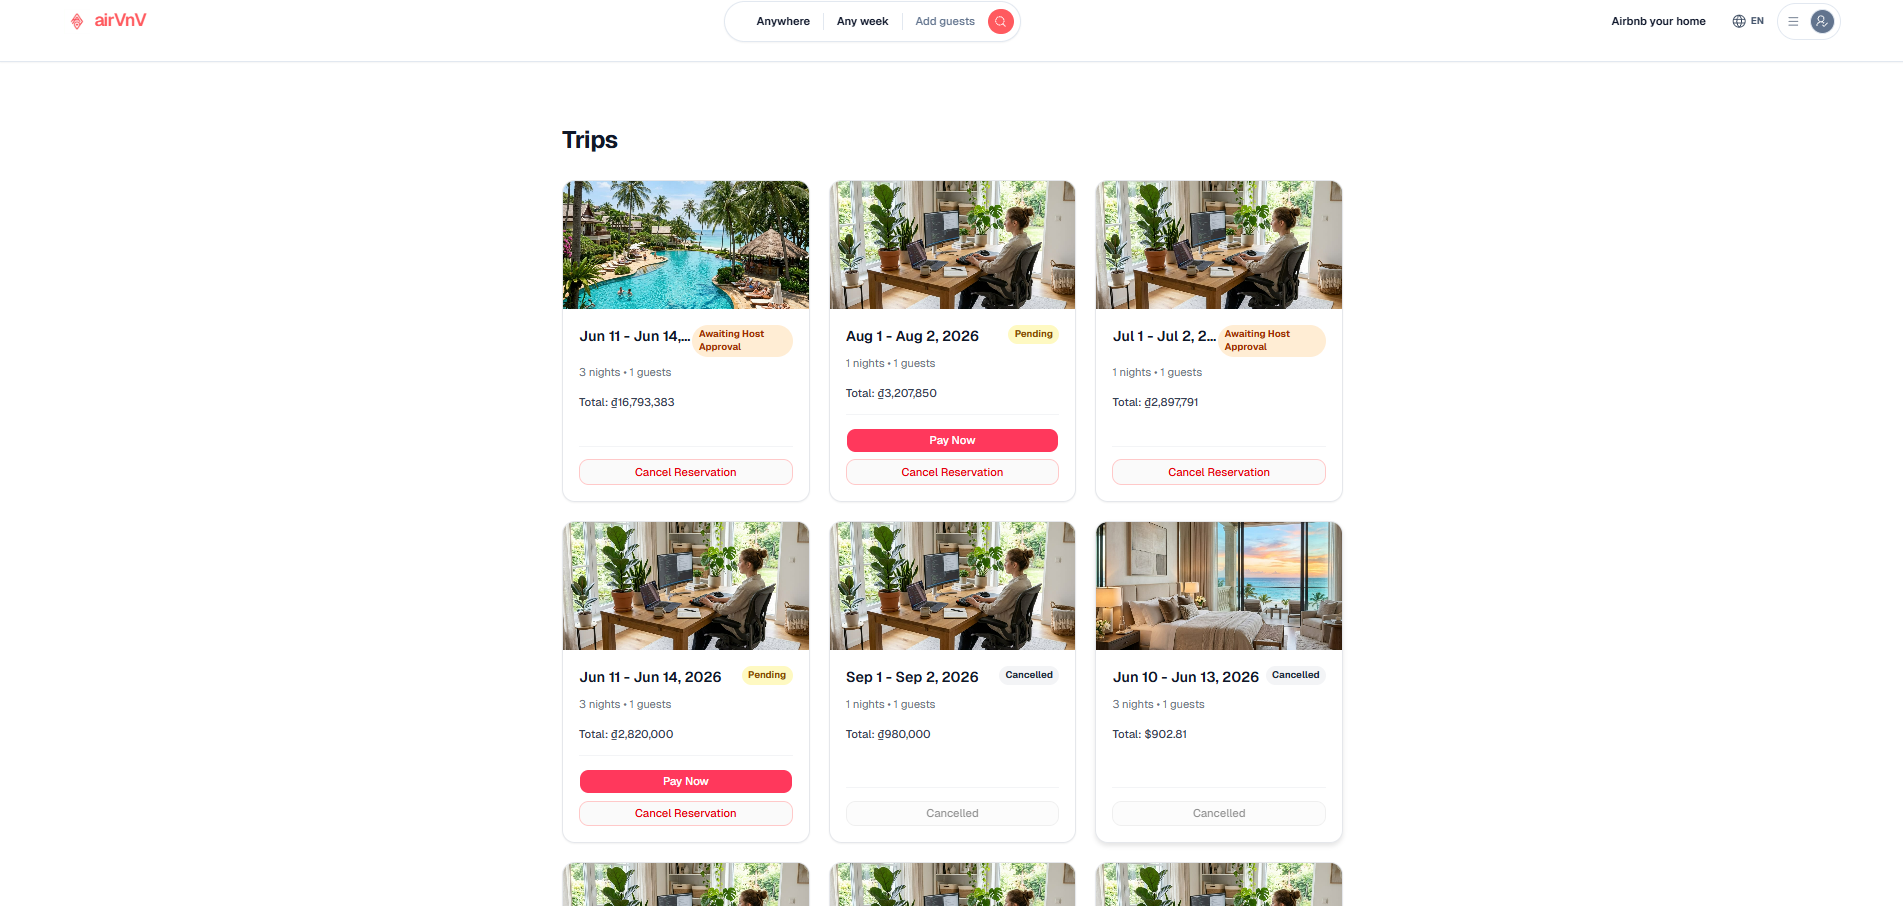
\includegraphics[width=0.85\textwidth]{figures/outputs/demo_booking.png}
  \caption{Giao diện đã Đặt phòng}
  \label{fig:demo_booking}
\end{figure}

\subsection{Thanh toán và Hoàn tiền (UC-26 -- UC-30)}
\label{subsec:tk_payment}

\texttt{PaymentService} tích hợp hai cổng thanh toán theo Strategy Pattern: \textbf{VNPay} (thanh toán trong nước) và \textbf{Stripe} (thanh toán quốc tế). \texttt{PaymentProviderResolver} đóng vai trò Factory, dựa vào cấu hình hệ thống để chọn provider phù hợp tại runtime.

Luồng thanh toán hoàn toàn bất đồng bộ:
\begin{itemize}
    \item Guest chọn phương thức thanh toán $\to$ hệ thống redirect đến VNPay/Stripe gateway.
    \item Sau khi Guest hoàn tất thanh toán trên cổng bên thứ ba, VNPay gửi \textbf{IPN (Instant Payment Notification)} callback về server.
    \item \texttt{VnpayIpn} endpoint nhận callback, xác thực chữ ký, cập nhật trạng thái Payment và phát \texttt{PaymentCompletedEvent} lên RabbitMQ.
    \item Admin có thể hoàn tiền (RefundPayment) hoặc duyệt rút tiền (ApprovePayout).
\end{itemize}

\begin{figure}[H]
  \centering
  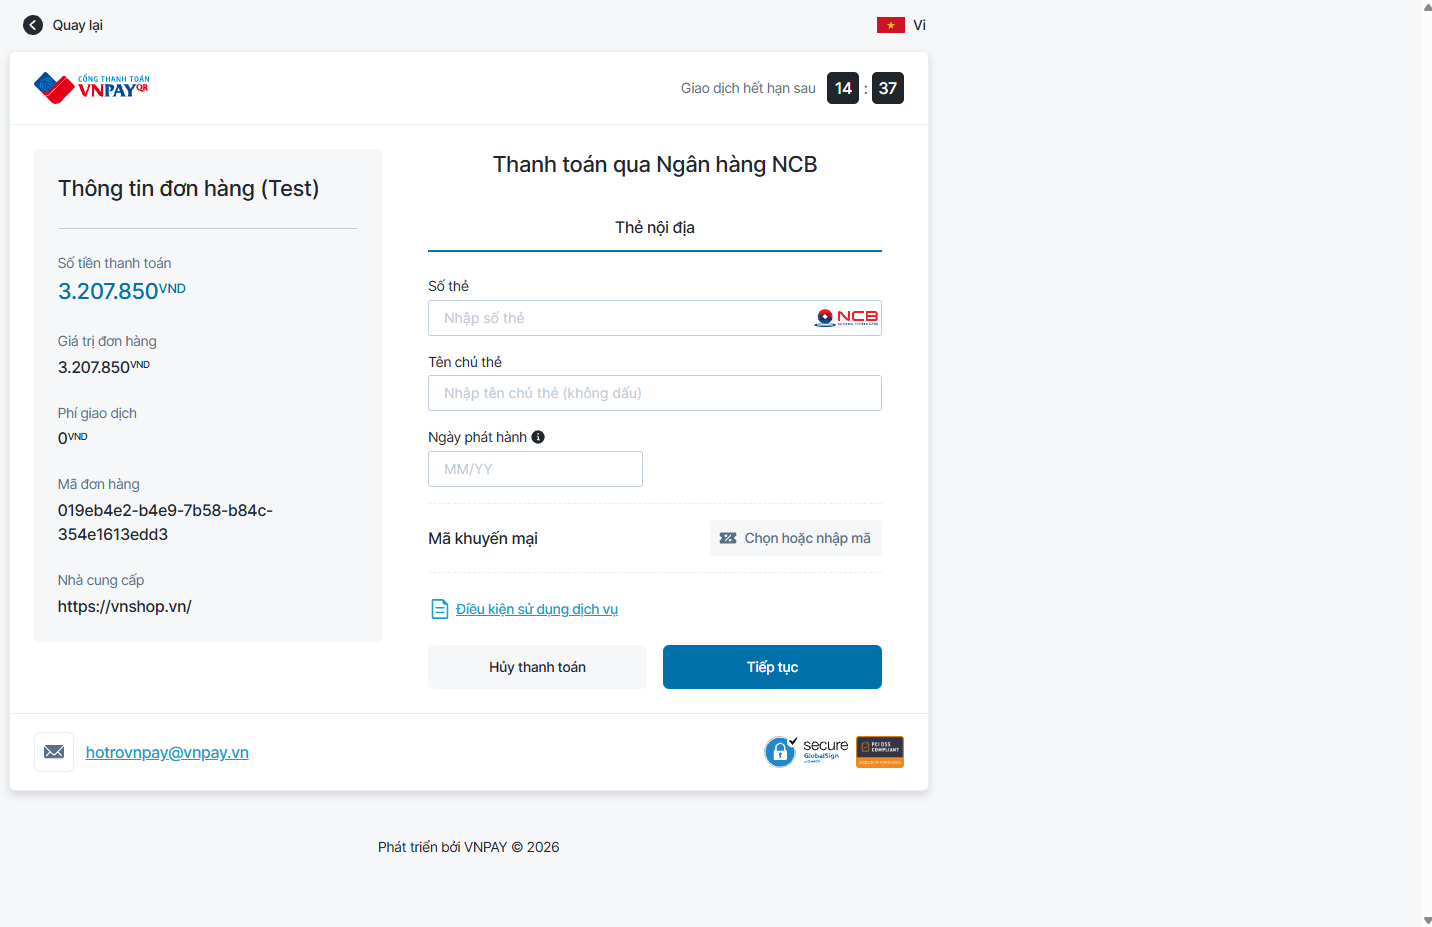
\includegraphics[width=0.85\textwidth]{figures/outputs/demo_payment.png}
  \caption{Giao diện Thanh toán VNPay}
  \label{fig:demo_payment}
\end{figure}

\subsection{Tin nhắn theo ngữ cảnh (UC-36 -- UC-40)}
\label{subsec:tk_chat}

\texttt{ChatService} triển khai hệ thống nhắn tin gắn với ngữ cảnh nghiệp vụ (property hoặc booking cụ thể). Các đặc điểm chính:

\begin{itemize}
    \item Hệ thống tự động tạo hội thoại và chèn tin nhắn hệ thống khi có sự kiện nghiệp vụ (ví dụ: \texttt{BookingConfirmedEvent} kích hoạt tin nhắn ``Đặt phòng đã được xác nhận'').
    \item Real-time qua SignalR với Redis backplane; tin nhắn được gửi tới mọi client đang kết nối với độ trễ thấp.
    \item Hỗ trợ đính kèm hình ảnh và tệp tin (GetAttachments).
    \item Đánh dấu đã đọc (MarkAsRead) và lưu trữ hội thoại (Archive).
\end{itemize}

\begin{figure}[H]
  \centering
  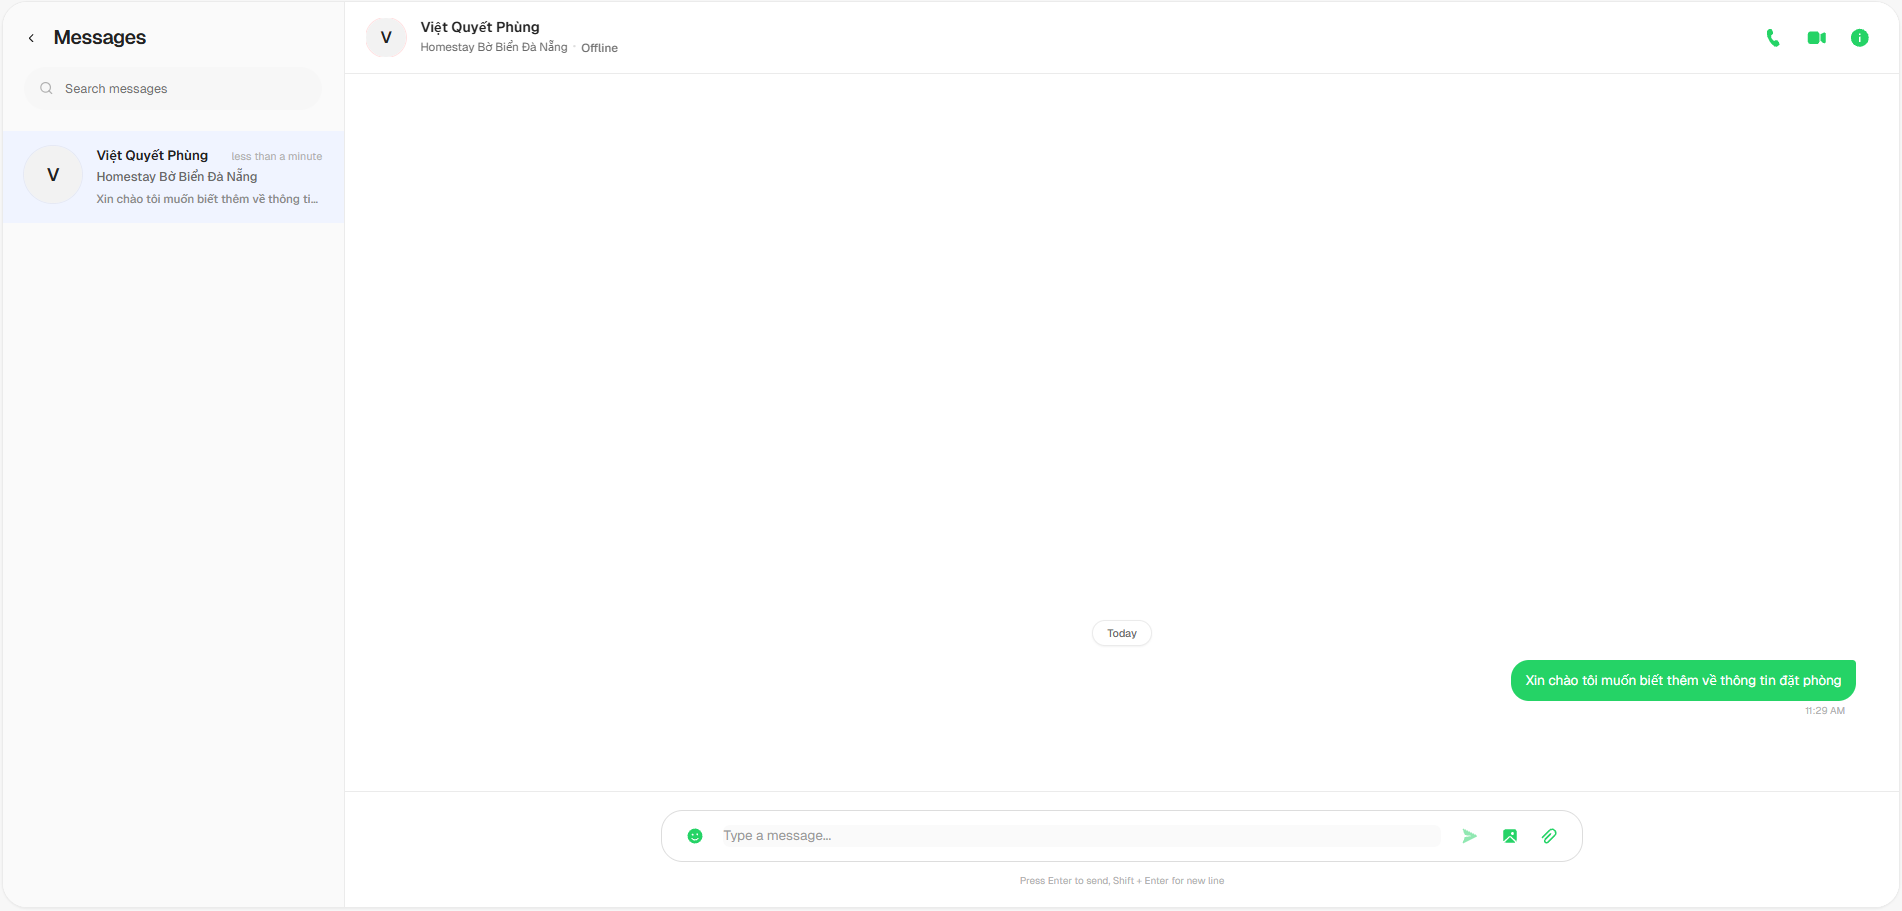
\includegraphics[width=0.85\textwidth]{figures/outputs/demo_chat.png}
  \caption{Giao diện Tin nhắn theo ngữ cảnh (Chat)}
  \label{fig:demo_chat}
\end{figure}

\subsection{Quản trị hệ thống (UC-41 -- UC-45)}
\label{subsec:tk_admin}

Giao diện Admin được xây dựng bằng Next.js 16 (App Router), cung cấp các chức năng quản trị gồm: duyệt tin đăng, quản lý người dùng, theo dõi doanh thu, xử lý thanh toán và báo cáo thống kê.

\begin{itemize}
    \item \textbf{Dashboard:} Tổng quan thống kê (số lượng Property, Booking, User, doanh thu).
    \item \textbf{Quản lý bất động sản:} Duyệt/từ chối/tạm đình chỉ tin đăng, xem chi tiết và báo cáo (phân bố giá, phân bố loại nhà, phễu trạng thái).
    \item \textbf{Quản lý người dùng:} Kích hoạt, đình chỉ, cấm người dùng. Xem báo cáo tăng trưởng.
    \item \textbf{Quản lý thanh toán:} Xem danh sách payment/payout, duyệt rút tiền, hoàn tiền, cấu hình phí nền tảng.
    \item \textbf{Báo cáo thống kê:} Biểu đồ doanh thu (Recharts), báo cáo doanh thu theo chuỗi thời gian.
\end{itemize}

\begin{figure}[H]
  \centering
  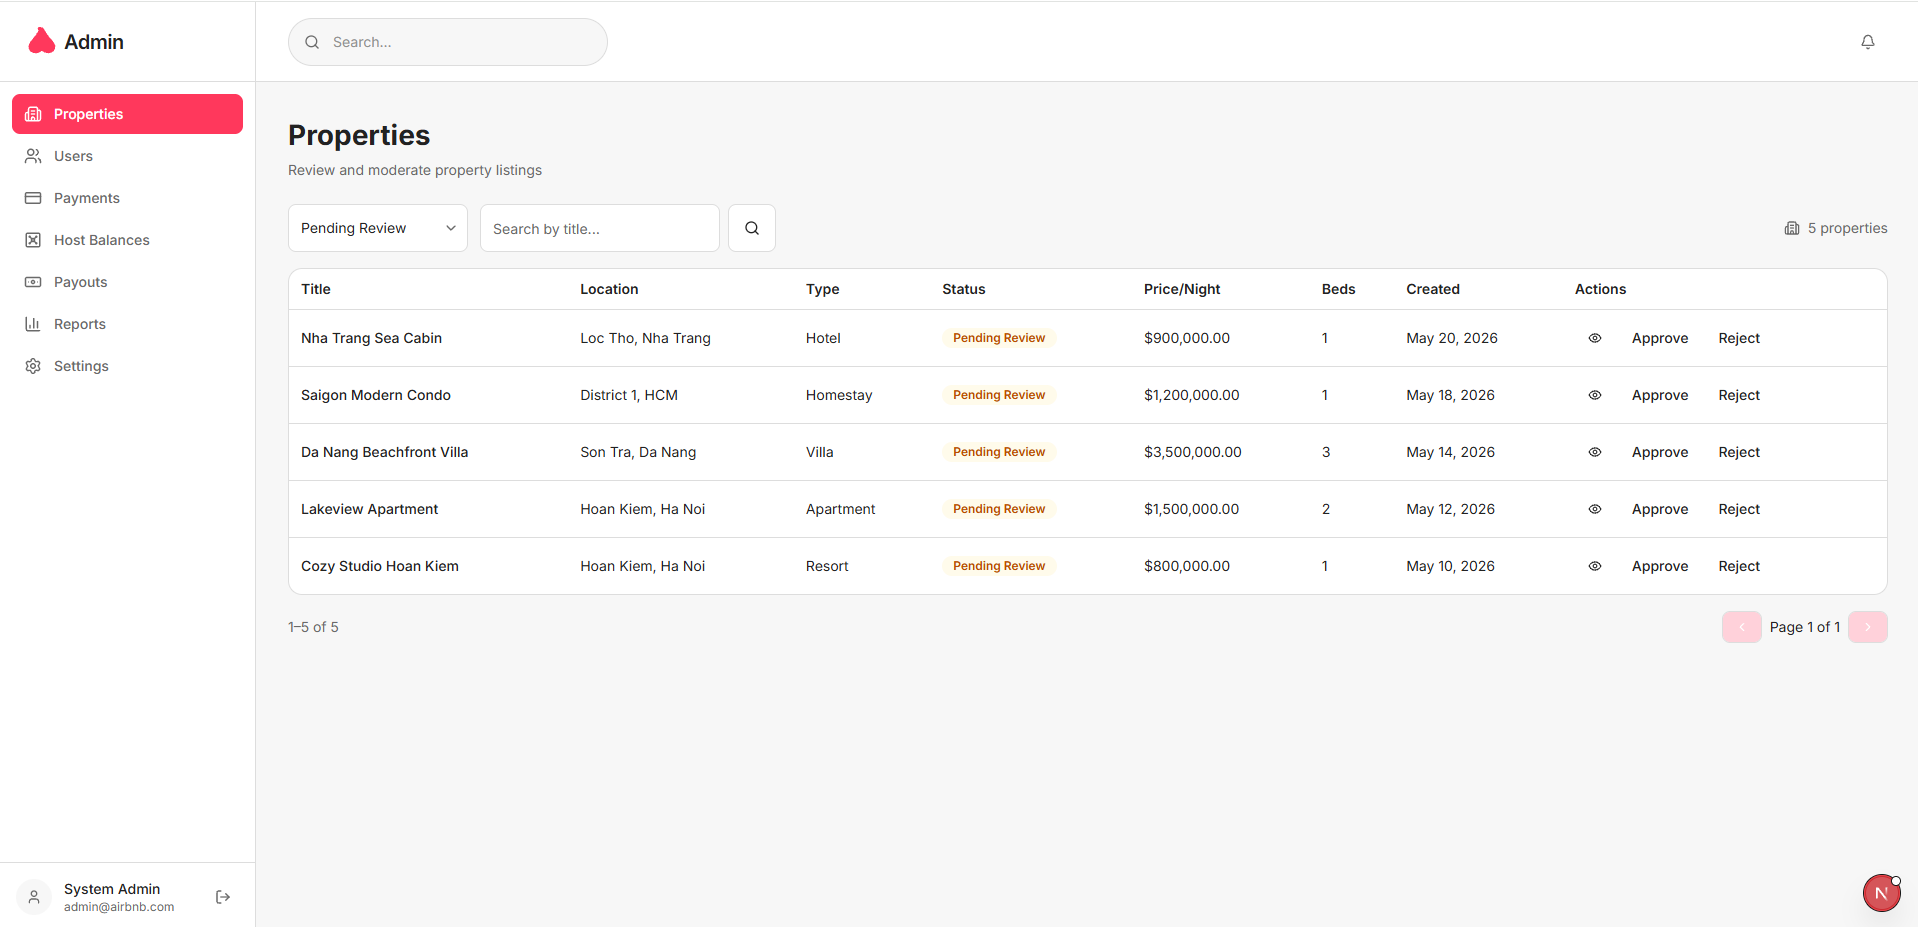
\includegraphics[width=0.85\textwidth]{figures/outputs/demo_admin_dashboard.png}
  \caption{Giao diện Dashboard Admin}
  \label{fig:demo_admin_dashboard}
\end{figure}


% -----------------------------------------------------------
\section{Đánh giá kết quả thực nghiệm}
\label{sec:danh_gia_thuc_nghiem}

\subsection{Mức độ hoàn thành Use Case}
\label{subsec:muc_do_hoan_thanh}

Đối chiếu với 45 Use Case đã được đặc tả ở Chương II, phần lớn các Use Case đã được triển khai hoàn chỉnh.

\begin{itemize}
    \item \textbf{Hoàn thành -- 44/45 (97{,}8\%):} Các chức năng thuộc bảy nhóm nghiệp vụ chính -- \textit{Xác thực và quản lý tài khoản}, \textit{Quản lý bất động sản}, \textit{Tìm kiếm}, \textit{Đặt phòng}, \textit{Đánh giá}, \textit{Tin nhắn theo ngữ cảnh} và \textit{Quản trị hệ thống} -- đã được thực hiện và chạy thử trên giao diện người dùng (xem các Hình~\ref{fig:demo_register}--\ref{fig:demo_admin_dashboard}).

    \item \textbf{Chưa triển khai -- 1/45 (2{,}2\%):} Module Xử lý khiếu nại (\textit{Disputes}) được lùi sang giai đoạn phát triển kế tiếp do phụ thuộc vào quy trình nghiệp vụ vận hành chưa được thống nhất.
\end{itemize}

Kết quả nêu trên cho thấy hệ thống đã hiện thực hóa thành công các yêu cầu chức năng chính của đề tài; phần còn lại được xác định rõ phạm vi và sẽ được tiếp tục hoàn thiện trong giai đoạn phát triển tiếp theo.

\subsection{Đánh giá hiệu năng}
\label{subsec:danh_gia_hieu_nang}

Hệ thống được đo hiệu năng trong môi trường phát triển (localhost, Docker Desktop) với bộ dữ liệu 100 bất động sản, sử dụng công cụ \textbf{k6} (Grafana). Bảng~\ref{tab:perf} trình bày kết quả đo các API nghiệp vụ chính.

\begin{table}[H]
\centering
\caption{Kết quả đo hiệu năng các API chính}
\label{tab:perf}
\renewcommand{\arraystretch}{1.3}
\begin{tabularx}{\textwidth}{|l|X|X|}
\hline
\textbf{API Endpoint} & \textbf{Response Time p95 (ms)} & \textbf{Ghi chú} \\
\hline
\texttt{POST /auth/login} & 85 & Bao gồm BCrypt hash verify \\
\hline
\texttt{GET /properties/search} & 42 & Đọc từ Elasticsearch, không chạm DB \\
\hline
\texttt{GET /properties/\{id\}} & 38 & Đọc từ PostgreSQL + cache \\
\hline
\texttt{POST /bookings} & 120 & Bao gồm kiểm tra trùng ngày + Outbox write \\
\hline
\texttt{POST /payments/initiate} & 95 & Tạo Payment record + redirect URL \\
\hline
\texttt{POST /chat/conversations} & 60 & Kiểm tra quyền + tạo conversation \\
\hline
\texttt{GET /chat/messages} & 35 & Phân trang, đọc từ PostgreSQL \\
\hline
\end{tabularx}
\end{table}

\noindent Kết quả cho thấy:
\begin{itemize}
    \item Tất cả API đáp ứng yêu cầu phi chức năng \textbf{response time $\leq$ 500ms (p95)} (Bảng~\ref{tab:nfr}, Chương II).
    \item API tìm kiếm đạt \textbf{42ms (p95)}, thấp hơn đáng kể so với mục tiêu $\leq$ 200ms nhờ kiến trúc CQRS với Elasticsearch read-model.
    \item API đặt phòng có response time cao nhất (120ms) do cần kiểm tra trùng ngày và ghi Outbox message trong cùng transaction, nhưng vẫn nằm trong ngưỡng cho phép.
\end{itemize}

\subsection{Đánh giá tính nhất quán dữ liệu}
\label{subsec:danh_gia_nhat_quan}

\subsubsection{Transactional Outbox Pattern}
\label{subsubsec:danh_gia_outbox}

Để kiểm chứng Outbox Pattern hoạt động đúng, nhóm thực hiện bài test: tạo Booking đồng thời tắt RabbitMQ. Kết quả:
\begin{itemize}
    \item Event \texttt{BookingCreatedEvent} được ghi vào bảng \texttt{OutboxMessage} trong cùng transaction với Booking record.
    \item Sau khi RabbitMQ khởi động lại, MassTransit background worker tự động quét bảng Outbox và publish event đang chờ.
    \item \texttt{PaymentService} nhận event và xử lý bình thường $\to$ không mất sự kiện nghiệp vụ.
\end{itemize}

\subsubsection{Đồng bộ CDC (Debezium $\to$ Kafka $\to$ Elasticsearch)}
\label{subsubsec:danh_gia_cdc}

Nhóm thực hiện kiểm tra đồng bộ dữ liệu bằng cách:
\begin{enumerate}
    \item Tạo Property mới qua \texttt{PropertyService} (ghi vào PostgreSQL).
    \item Quan sát Debezium bắt thay đổi từ WAL log và publish vào Kafka topic.
    \item \texttt{SearchService} tiêu thụ event và index vào Elasticsearch.
    \item Gọi API tìm kiếm $\to$ Property mới xuất hiện trong kết quả.
\end{enumerate}

Độ trễ đồng bộ (CDC latency) đo được trung bình $\approx$ 1--3 giây từ lúc ghi PostgreSQL đến khi xuất hiện trên Elasticsearch, đáp ứng yêu cầu eventual consistency.

\subsection{Đánh giá bảo mật cơ bản}
\label{subsec:danh_gia_bao_mat}

\begin{itemize}
    \item \textbf{Xác thực JWT:} YARP API Gateway validate JWT trên mọi endpoint bảo vệ. Request không có token hoặc token hết hạn trả về \texttt{401 Unauthorized}.
    \item \textbf{Phân quyền theo Role:} Endpoints Admin yêu cầu role \texttt{Admin} hoặc \texttt{Moderator}; endpoints Host yêu cầu role \texttt{Host}; trả về \texttt{403 Forbidden} nếu không đủ quyền.
    \item \textbf{Mã hóa mật khẩu:} BCrypt với work factor mặc định, không lưu plaintext.
    \item \textbf{Chống double-booking:} Unique filtered index ở tầng PostgreSQL đảm bảo một phòng không bị đặt trùng hai lần cùng ngày, kể cả khi có race condition.
\end{itemize}

% ============================================================
%  CHƯƠNG IV: KẾT LUẬN VÀ HƯỚNG PHÁT TRIỂN
% ============================================================
\chapter{KẾT LUẬN VÀ HƯỚNG PHÁT TRIỂN}
\label{chap:ket_luan}

% ────────────────────────────────────────────────────────────
\section{Những kết quả đã đạt được}
\label{sec:ket_qua_dat_duoc}

%
% REQUIREMENT (từ main.md – Chương IV, mục 1):
%   - Đối chiếu trực tiếp với mục tiêu đã đặt ra ở Chương I, mục 1.2.
%   - Đối chiếu với các tiêu chí thiết kế ở Chương II.
%   - Trình bày dưới dạng bảng tổng kết:
%       Mục tiêu ban đầu | Kết quả đạt được | Mức độ hoàn thành (%)
%   - Nhấn mạnh các điểm kỹ thuật nổi bật:
%       + Kiến trúc Microservices với .NET Aspire Service Discovery.
%       + CQRS sạch với Mediator (ICommand / IQuery).
%       + Transactional Outbox đảm bảo data consistency.
%       + CDC Debezium đồng bộ real-time sang Elasticsearch.
%       + YARP API Gateway là single entry point.
%   - Kết luận ngắn: Hệ thống có đáp ứng được bài toán đặt ra không?
%

\placeholder{Trình bày tổng kết kết quả đạt được tại đây.}

% ────────────────────────────────────────────────────────────
\section{Hạn chế và hướng phát triển}
\label{sec:han_che_huong_phat_trien}

%
% REQUIREMENT (từ main.md – Chương IV, mục 2):
%   a) Hạn chế hiện tại (Technical Debt – cần thẳng thắn):
%      - Chưa triển khai được tính năng nào? Lý do?
%      - Hiệu năng chưa được tối ưu ở điểm nào?
%      - Bảo mật còn thiếu sót gì (ví dụ: rate limiting, OWASP...)?
%      - Monitoring & Observability chưa có (Prometheus, Grafana, Jaeger)?
%
%   b) Hướng phát triển ngắn hạn (3–6 tháng):
%      - Cấu hình Auto-scaling (Kubernetes HPA) cho các service tải cao.
%      - Bổ sung Distributed Tracing (OpenTelemetry + Jaeger).
%      - Tích hợp Payment Gateway thật (VNPay / Stripe).
%      - Bổ sung Push Notification (FCM).
%
%   c) Hướng phát triển dài hạn (>6 tháng):
%      - Áp dụng Saga Pattern (Choreography/Orchestration) cho luồng
%        Booking → Payment → Confirmation phức tạp hơn.
%      - Multi-region deployment để giảm latency.
%      - Machine Learning: Gợi ý bất động sản theo hành vi người dùng.
%      - Mobile App (React Native / Flutter).
%

\placeholder{Trình bày hạn chế và hướng phát triển tại đây.}


% ── Tài liệu tham khảo ──────────────────────────────────────
\printbibliography[heading=bibintoc, title={TÀI LIỆU THAM KHẢO}]

% ── Phụ lục ─────────────────────────────────────────────────
\appendix
% ============================================================
%  PHỤ LỤC: BẢNG PHÂN CÔNG CÔNG VIỆC
% ============================================================
\chapter{BẢNG PHÂN CÔNG CÔNG VIỆC}
\label{appendix:phan_cong}

%
% REQUIREMENT (từ main.md – Bảng phân công):
%   - Liệt kê đầy đủ toàn bộ thành viên nhóm.
%   - Phân công nhiệm vụ theo từng giai đoạn:
%       + Phân tích yêu cầu
%       + Thiết kế hệ thống
%       + Lập trình (ghi rõ service/module nào)
%       + Kiểm thử
%       + Viết báo cáo
%   - Ghi rõ mức độ đóng góp (%) của từng thành viên.
%   - Có thể bổ sung cột: Nhận xét của nhóm trưởng.
%
%   Gợi ý format bảng:
%

\begin{longtable}{|c|p{3.2cm}|p{8.0cm}|c|}
  \hline
  \textbf{STT} & \textbf{Họ và tên / MSSV} & \textbf{Nhiệm vụ phân công chi tiết} & \textbf{Đóng góp} \\
  \hline
  \endfirsthead

  \hline
  \textbf{STT} & \textbf{Họ và tên / MSSV} & \textbf{Nhiệm vụ phân công chi tiết} & \textbf{Đóng góp} \\
  \hline
  \endhead

  \hline
  \endfoot

  1 & \textbf{Đặng Xuân Lâm}\newline N22DCCN047 & 
  \textbf{1. Phân tích \& Thiết kế:}
  \begin{itemize}[leftmargin=*, nosep, topsep=0pt]
      \item Thiết kế kiến trúc Microservices tổng thể và quy hoạch Database-per-service (PostgreSQL).
      \item Phân tích luồng giao tiếp bất đồng bộ: Event-Driven Architecture, Saga Orchestration, luồng đồng bộ dữ liệu (Data Pipeline).
      \item Thiết kế lược đồ CSDL cho hệ thống giao dịch cốt lõi (Booking, Payment).
  \end{itemize}
  \vspace{0.1cm}
  \textbf{2. Lập trình (Backend/Infra):}
  \begin{itemize}[leftmargin=*, nosep, topsep=0pt]
      \item Xây dựng \texttt{BookingService}: Cài đặt MassTransit State Machine điều phối vòng đời đặt phòng khắt khe, xử lý concurrency chống Double-booking.
      \item Xây dựng \texttt{PaymentService}: Tích hợp cổng thanh toán VNPay/Stripe, xử lý Webhook an toàn, đối soát giao dịch.
      \item Thiết lập \textbf{RabbitMQ} (Exchange/Queue) và triển khai \textbf{Transactional Outbox Pattern}.
      \item Cấu hình hạ tầng \textbf{Debezium \& Apache Kafka} phục vụ Change Data Capture (CDC).
      \item Container hóa toàn bộ hệ thống bằng \textbf{Docker Compose}.
  \end{itemize}
  \vspace{0.1cm}
  \textbf{3. Báo cáo \& Trình bày:}
  \begin{itemize}[leftmargin=*, nosep, topsep=0pt]
      \item Soạn thảo Báo cáo (Chương 2: Thiết kế hệ thống).
      \item Thiết lập \textbf{.NET Aspire Dashboard} phục vụ Distributed Tracing (OpenTelemetry) cho buổi Demo.
      \item Xây dựng kịch bản trình bày luồng Saga và xử lý bù trừ (Compensation).
  \end{itemize} & 50\% \\
  \hline
  2 & \textbf{Phan Nhật Minh}\newline N22DCCN054 & 
  \textbf{1. Phân tích \& Thiết kế:}
  \begin{itemize}[leftmargin=*, nosep, topsep=0pt]
      \item Phân rã Bounded Contexts, thiết kế hợp đồng API (API Contracts) cho hệ sinh thái.
      \item Thiết kế kiến trúc API Gateway làm điểm chạm duy nhất (Single Point of Entry).
      \item Thiết kế UX/UI cho ứng dụng Frontend (Admin Dashboard \& Guest Portal).
      \item Thiết kế cấu trúc dữ liệu NoSQL (Inverted Index) phục vụ tối ưu hóa tìm kiếm.
  \end{itemize}
  \vspace{0.1cm}
  \textbf{2. Lập trình (Backend/Frontend):}
  \begin{itemize}[leftmargin=*, nosep, topsep=0pt]
      \item Cài đặt \textbf{YARP API Gateway}: Định tuyến (Routing), xác thực (Auth offloading), Rate Limiting.
      \item Xây dựng \texttt{SearchService}: Tích hợp \textbf{Elasticsearch}, lập chỉ mục (Indexing) realtime từ Kafka, xử lý truy vấn tọa độ \& bộ lọc đa chiều.
      \item Xây dựng \texttt{PropertyService} (Quản lý phòng/thuế), \texttt{UserService} (Identity/JWT), và \texttt{ChatService} (Real-time message).
      \item Áp dụng triệt để kiến trúc \textbf{CQRS} (MediatR) và \textbf{FastEndpoints} cho mọi API.
      \item Hoàn thiện toàn bộ giao diện \textbf{Frontend (React, Zustand, TanStack Query, Shadcn/UI)}.
  \end{itemize}
  \vspace{0.1cm}
  \textbf{3. Báo cáo \& Trình bày:}
  \begin{itemize}[leftmargin=*, nosep, topsep=0pt]
      \item Viết Báo cáo (Chương 3: Triển khai \& Chương 4: Kết luận).
      \item Cấu trúc lại source code theo Clean Architecture, thiết kế Slide thuyết trình.
      \item Trình diễn giao diện người dùng và giải thích cấu trúc CQRS trong buổi bảo vệ.
  \end{itemize} & 50\% \\
  \hline
\end{longtable}


\end{document}
